\chapter{荷侧先进绝热压缩空气能量枢纽建模及运行方法}
\label{cha:st-caes}

\section{概述}
\label{sec:intro}
能量枢纽具备(燃)气、热、电等多能流载体间的传递、转换及存储功能,是综合能源系统灵活性的重要体现。随着电气化供暖技术的普遍采用,区域配电网与区域供热管网将通过具备热电联供与热电联储能力的能量枢纽紧密耦合,从而实现电能(易输不易储)与热能(易储不易输)的互补,促进可再生能源电力的热电多能流协同消纳。第~\ref{cha:simulation}章提及蓄热系统通过空气压缩热能的收集、存储与回馈,使得~AA-CAES~具备了热电联产与热电联储的能力,成为潜在的热电能量枢纽
\cite{EH-Concept-07, EH-FREEDM-11},本章将从负荷侧以能量枢纽的视角挖掘AA-CAES的供能灵活性。

%第~\ref{cha:intro}章指出从源-网-荷三侧挖掘~AA-CAES~提供的常规灵活性、供能灵活性及接口灵活性,第~\ref{cha:aa-caes}章从网侧实现了基于~AA-CAES~技术的储能电站解决方案。

采用AA-CAES构建热电能量枢纽一般有两种思路,第一种思路为改造或扩展AA-CAES内部的热力循环或回热系统,使其具备更灵活的热电联供与热电联储能力,进而构建用于分布式多能联供场景的小型能量枢纽,该能量枢纽与所接入的配电网络及供热管网一般由园区级或社区级能源集成商集中运营;第二种思路是将AA-CAES视为大型能量枢纽(或集成站)内部的清洁电能存储部件,充分发挥其具有的大容量、长循环寿命等优点,以与集成站内部的热电联产机组、(电)热泵等部件实现全寿命周期的匹配,该类能量枢纽一般由独立于热网及电网的第三方主体运营管理\footnote{从AA-CAES内部储热组件的视角而言,第一种思路需要的储热单元容量较大,而第二种思路只需设计与供电相匹配的储热组件容量即可。}。本章将针对这两类AA-CAES型热电能量枢纽展开研究,分析其内部供能特性及对外热电联供特性的相互制约关系,并分析集中运营与独立运营两种环境下AA-CAES 型能量枢纽的调度运行及市场运营等问题,以充分发挥AA-CAES在热电联供场景下的供能灵活性。

本章结构安排如图\ref{fig:Hub-Flow-Chart}所示,第\ref{sec:struc-EH-CAES}节设计两类典型的AA-CAES型热电联供能量枢纽,并建立AA-CAES型能量枢纽的热电联供与热电联储模型;第\ref{sec:st-caes-dispatch}节研究含AA-CAES型能量枢纽的热电综合能源系统的调度问题,以充分发挥多能联供型能量枢纽的供能灵活性;第
\ref{sec:exergy-IES-model}节建立基于㶲理论的热电综合能源系统质量-数量联合模型,实现热电不同品位能流的差异化建模;第\ref{sec:bid-st-caes}节研究面向热电综合能源市场的能量枢纽市场竞标策略,挖掘AA-CAES型能量枢纽的热电综合能源市场交叉套利,以提升能量枢纽的运行经济性。

\begin{figure}[H] % use float package if you want it here
  \centering
  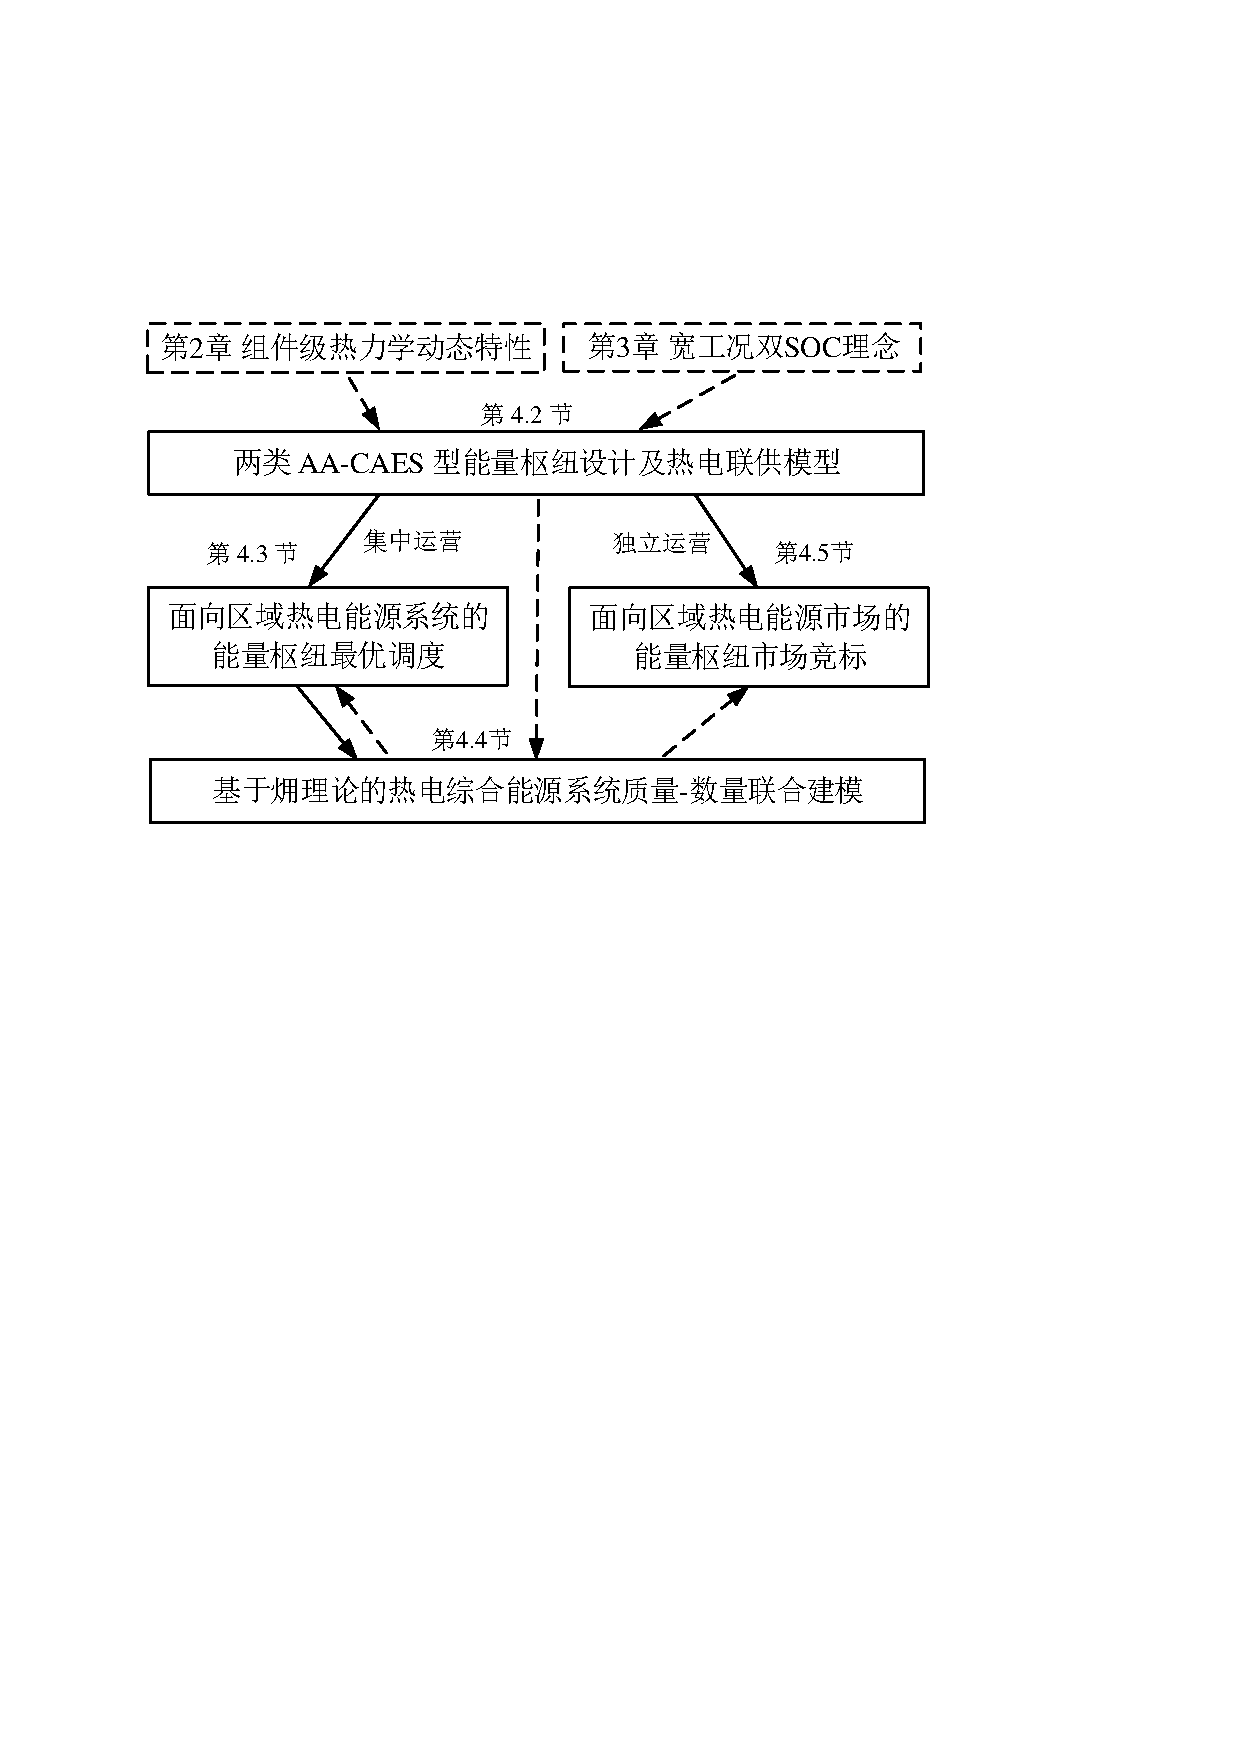
\includegraphics[scale=0.85]{figures/Chap4-1-Hub-Flow-Chart-V3.pdf}
  \caption{第4章组织结构安排}
  \label{fig:Hub-Flow-Chart}
\end{figure}

\section{先进绝热压缩空气储能能量枢纽设计及建模}
\label{sec:struc-EH-CAES}
目前已存在多种具有灵活工作模式的热电联供型AA-CAES或CAES系统,如CAES与燃气轮机构成的混合循环系统\cite{CAES-Concepts-Review-10}、AA-CAES与槽式集热构成的混合系统\cite{ST-CAES-CXT-18,ST-CAES-17}、风-光-CAES互补系统\cite{Thermo-WSCAES-17}、电阻丝与AA-CAES 配合构成的高温混合CAES系统\cite{Hybrid-CAES-14, HTH-CAES-Berk-18}、CAES 与制冷循环耦合系统\cite{CAES-Refri-06}、CAES与内燃机循环耦合系统\cite{CAES-Inner-Comb-06} 等等。本节基于该类混合型AA-CAES系统抽象出两类典型的AA-CAES型热电能量枢纽,一类为无碳排的AA-CAES型能量枢纽,另一类为大型AA-CAES能量枢纽(或集成站)。%同时建立两类能量枢纽的热电联供运行模型。

\subsection{AA-CAES型能量枢纽设计}

\textbf{(1)~I~型AA-CAES能量枢纽}

针对中国等天然气资源受限地区,可以充分利用富余的新能源电力及AA-CAES的热电联供特性设计高效灵活的I型AA-CAES能量枢纽,如图~\ref{fig:AA-CAES-Hub-V1}~所示。I 型 AA-CAES能量枢纽在经典AA-CAES结构的基础上引入了CCHP系统中普遍采用的(电)热泵(Heat Pump,HP)为能流枢纽提供额外的热量供应,从而实现灵活的热电联供与热电联储。

I型AA-CAES对外可以供电与供热(制冷),其中制冷由透平排气提供(本文忽略制冷特性),对外供热热源一方面可取自电热泵,另一方面可取自压缩热收集系统。一般而言,热电能量枢纽需具备热能与电能的缓冲能力,I型能量枢纽的电能及热能缓冲功能均由内置的AA-CAES系统实现,即由储热罐实现热能缓冲,储气罐与储热罐共同提供电能缓冲作用。I型能量枢纽挖掘了AA-CAES固有的热电联供能力,主要用于分布式多能联供场景,由园区级配电网络及供热网运营商集中运营。

\begin{figure}[H] % use float package if you want it here
  \centering
  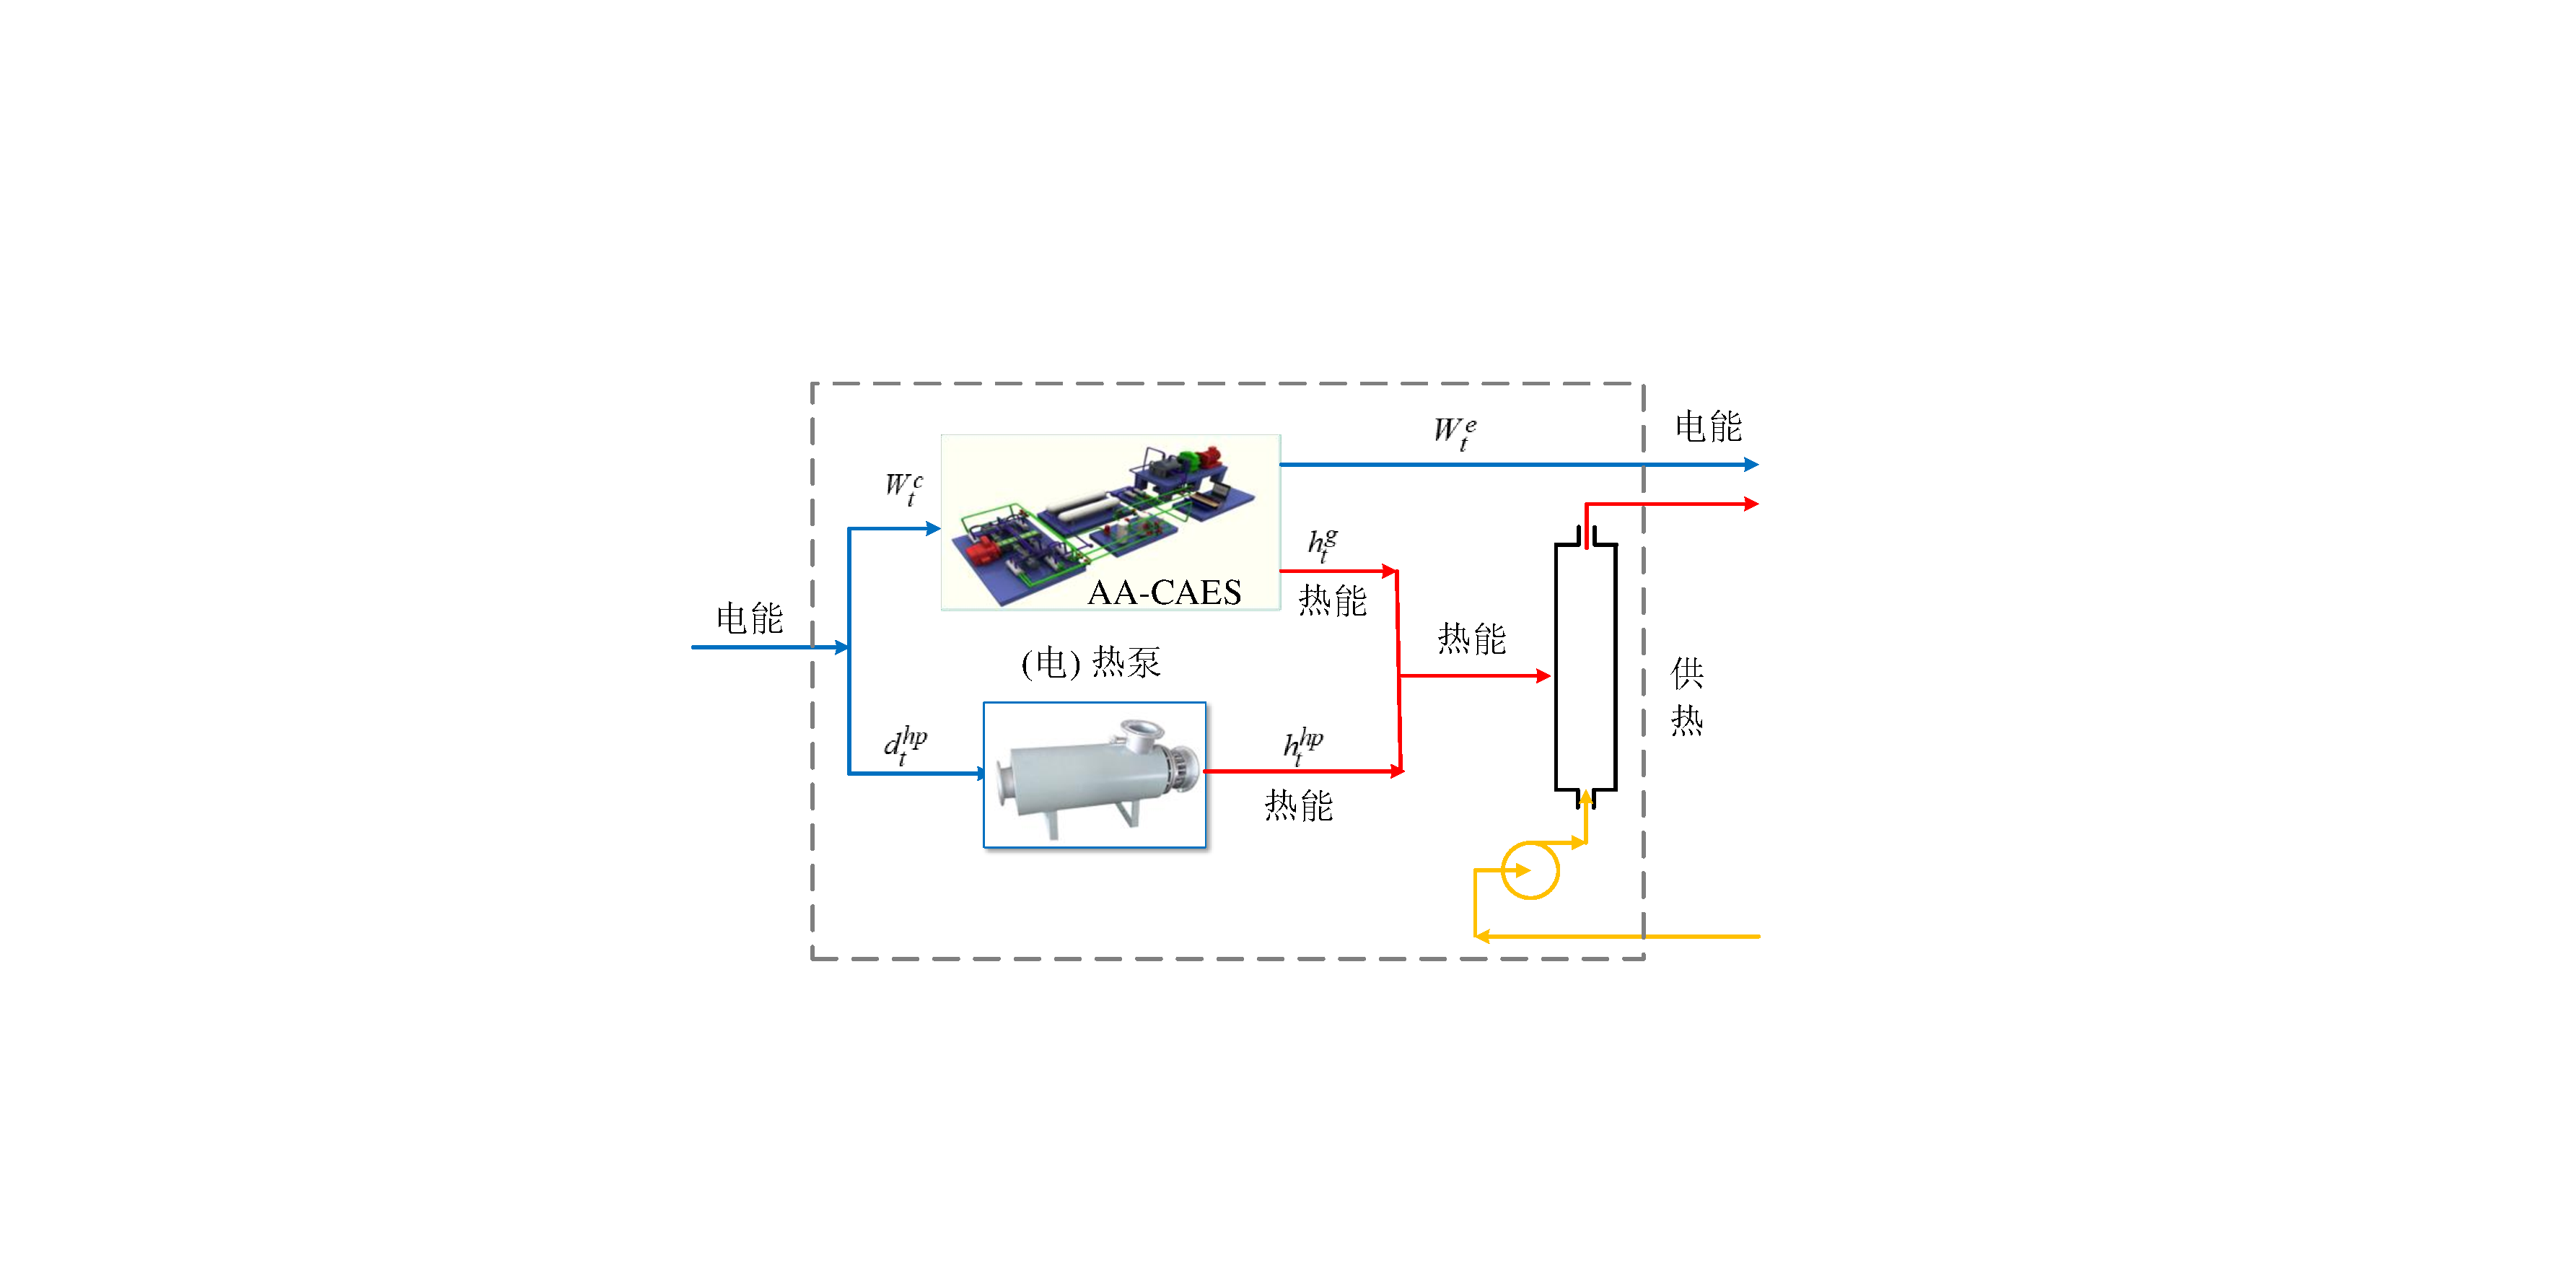
\includegraphics[scale=0.41]{figures/Chap4-2-AA-CAES-Hub-V1-3.pdf}
  \caption{~I~型AA-CAES能量枢纽结构}
  \label{fig:AA-CAES-Hub-V1}
\end{figure}

\textbf{(2)~II~型AA-CAES能量枢纽}

针对美国等页岩气开发技术成熟且具有明显经济优势的天然气资源丰富地区,可设计如图
~\ref{fig:AA-CAES-Hub-V2}~所示的II型AA-CAES能量枢纽\footnote{2016年,燃气机组超过火电等成为美国主力电源机组,而且将在相当长的一段时间内具有明显的成本优势,因此采用天然气作为II型AA-CAES能量枢纽的输入能源之一具有可行性,可参考https://energy.gov/downloads/download-staff-report-secretaryelectricity-markets-and-reliability}。其中,内置的AA-CAES 充当电能存储单元,由燃气驱动的CHP及由电能驱动的HP 为能量枢纽提供热能,而内置的TES则为能量枢纽提供热能的缓冲功能。

\begin{figure}[H] % use float package if you want it here
  \centering
  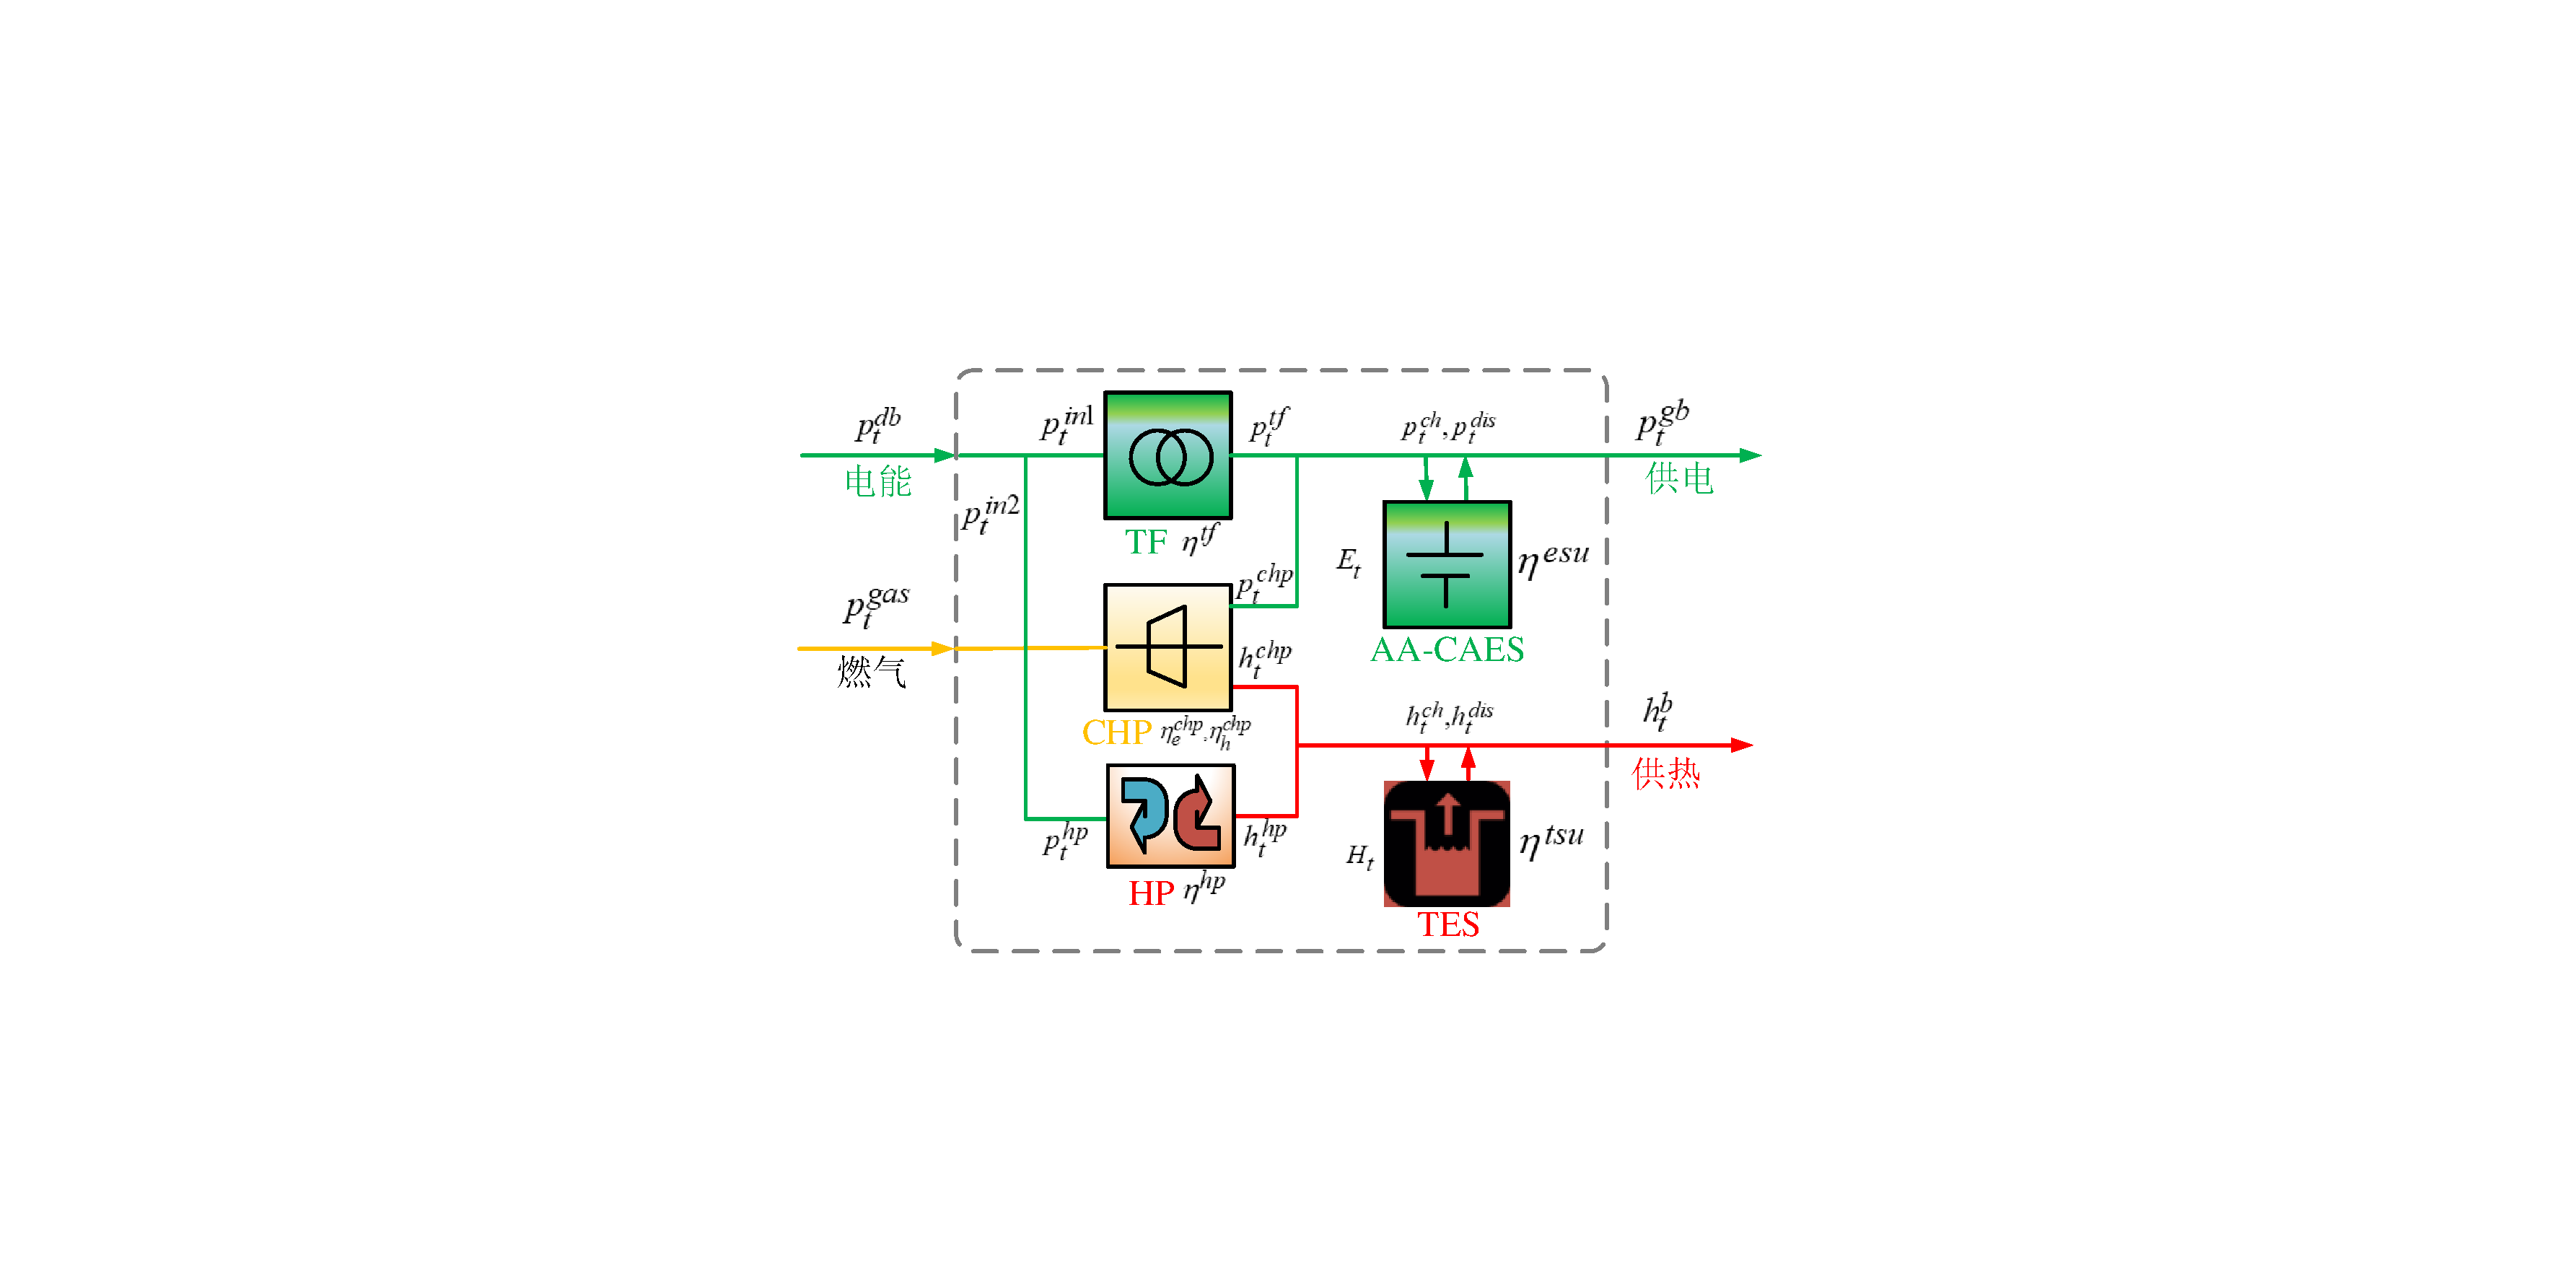
\includegraphics[scale=0.45]{figures/Chap4-2-AA-CAES-Hub-V3.pdf}
  \caption{~II~型AA-CAES能量枢纽结构}
  \label{fig:AA-CAES-Hub-V2}
\end{figure}

II型AA-CAES能量枢纽由于包含燃气与电能两个输入端,对外的供电既可取自电能输入,亦可取自内置的CHP,对外的供热既可取自内置的CHP,亦可取自内置的HP,从而可以充分利用电价、热价及燃料价格信息,实现灵活的内部能量管理;内置储热单元与储电单元的存在,使得II型AA-CAES能量枢纽具有更强的热电供能灵活性。II型能量枢纽基于AA-CAES 的长使用寿命及全生命周期成本优势等将AA-CAES 视为储电部件与CHP等组合形成能量枢纽,主要以第三方主体独立运营。

\subsection{AA-CAES型能量枢纽建模}
\label{sec:thermo-EH-CAES}
%AA-CAES型能量枢纽内含空气压缩机、换热网络、储热系统、储气室、透平发电机组,涉及热动、电动、气动等复杂过程。当前的压缩空气储能系统及能量枢纽建模多采用类似电池等储能系统的简化效率模型,难以刻画AA-CAES能量枢纽内部温度、压强等热动态,无法描述压缩机、透平等组件运行于部分负载工作点导致的变效率现象,无法满足区域热电综合能源系统中能量枢纽的变工况运行要求。
%I型与II型AA-CAES能量枢纽结构的不同,造成了二者不同的应用场景。I型能量枢纽由于内置的储能(储电、储热)单元少,供能灵活性弱于II型能量枢纽,主要用于以集中运行模式管理的园区或社区级热电综合能源系统。该类综合能源系统由于规模小,可实现无碳排运行,其中的所有能源基础设施由统一运营者调配,以充分利用系统中各灵活性分布式电源。与此相反,II型能量枢纽内置的储能单元多,供能灵活性更强,一般以第三方独立运营模式参与到热电综合能源系统的运行。本小节将给出两类能量枢纽的热电联供运行模型。

\textbf{(1) I型AA-CAES能量枢纽}

%本节采用文献~\inlinecite{ST-CAES-CXT-18}中的ST-CAES参数\footnote{由于本章设计的I型AA-CAES不完全等同于ST-CAES,因此对原文献的参数进行了适当修改。}分析本文设计的I 型AA-CAES 能量枢纽的热力学特性。

%此处说明双SOC模型对I型AA-CAES能量枢纽不大适用的问题,但可适用于II型AA-CAES能量枢纽。为此,此处重点针对I型能量枢纽进行热力学热性分析及对应的多能流建模。

在任一时段$t$,能量枢纽中AA-CAES消耗的电功率$W_t^c$由第2章中压缩机额定工况热力学模型(\ref{equ:comp-real-temp-2})-(\ref{equ:comp-pressure})给定,能量枢纽中AA-CAES提供的电功率$W_t^e$ 由第2章中膨胀机额定工况热力学模型(\ref{equ:turb-real-temp-2})-(\ref{equ:turb-pressure})给定。

对于用于区域综合能源系统的I型AA-CAES能量枢纽而言,其储气库一般会采用压力容器,储气库的温度会通过保温措施维持恒定。因此,储气库模型可以采用第\ref{cha:simulation}章中的VT模型(\ref{equ:Air-tank-model-VT}),即任一时刻$t$中储气库的储气压力SOC可以描述为,
\begin{subequations}
\label{eq:hub-pressure-SOC}
\begin{gather}
p_{t + 1}^{as} = p_{t}^{as} + \frac{1}{V_{as}}{R_g}T_t^{as}\left( {u_{t}^c \dot m_{t}^c - u_{t}^e \dot m_{t}^e} \right),\forall t\\
p_{min}^{as} \le p_{t}^{as} \le p_{max}^{as},\forall t
\end{gather}
\end{subequations}
其中,$p_{t}^{as}$ 为储气库压力水平;$T_t^{as}$ 为储气库内空气温度;$u_t^c$与$u_t^e$分别为表示压缩储能与膨胀释能运行状态的布尔量;其它变量或参数已在前文相关章节中定义\footnote{第3章至第5章主要研究面向电力系统运行的AA-CAES,需引入表示运行时段的角标$t$,导致相关变量的命名复杂。为简化变量符号,在不引起混淆的情况下,本章允许对变量上下标的相对位置做了适当调换。}。

相应地,储热水平可由(\ref{equ:TES-HTF-temp})简化为,
\begin{subequations}
\label{eq:hub-thermal-SOC}
\begin{gather}
H_{t}^{TES} = H_{t - 1}^{TES}(1-\gamma_H) + u_{t}^c h_{t}^c - u_{t}^e h_{t}^e - h_{t}^g,\forall t \label{eq:hub-thermal-SOC-Eq}\\
H_{min}^{TES} \le H_{t}^{TES} \le H_{max}^{TES},\forall t
\end{gather}
\end{subequations}
其中,$h_t^c$与$h^e$分别为压缩储能阶段的产热功率与膨胀释能阶段的耗热功率;$h_t^g$为AA-CAES为能量枢纽提供的对外供热功率。由电热泵提供的热功率为,
\begin{equation}
\label{equ:model-HP}
h_{t}^{hp} = \eta_{hp}d_{t}^{hp} \\
\end{equation}
其中,$h_{t}^{hp}$为热泵为能量枢纽提供的对外供热功率;$d_{t}^{hp}$为热泵消耗的电功率;$\eta_{hp}$为热泵效率。

事实上,I型AA-CAES能量枢纽的气热双储双SOC模型(\ref{eq:hub-pressure-SOC})及(\ref{eq:hub-thermal-SOC})与第~\ref{cha:aa-caes}章AA-CAES储能电站双SOC运行模型有异曲同工之妙。主要不同之处在于,I型AA-CAES相比于AA-CAES储能电站的容量较小,可采用压力容器等恒温储热模型,而在等温条件下第\ref{cha:aa-caes}章双SOC采用的储气动态与此处的压力动态一一对应。

\textbf{(2)II型AA-CAES能量枢纽}

II型AA-CAES能量枢纽由于内置了储热单元,同时具有燃气输入以及CHP等灵活性组件的支撑,其内部的AA-CAES储电单元受宽工况运行的影响较小,可以采用等效电池模型(或第\ref{cha:aa-caes}章中的双SOC能量模型)刻画运行特性。本节采用等效电池模型进行建模,以突出整个能量枢纽对外的热电联供特性。针对图~\ref{fig:AA-CAES-Hub-V2}所示的II 型AA-CAES能量枢纽,其热电联供运行模型为,
\begin{subequations}
\label{eq:EH-Cons-II}
\begin{gather}
p_t^{gb} = p_t^{in1} + p_t^{gas} \eta^{chp}_e + p_t^{dis} - p_t^{ch},~ \forall t  \label{eq:EH-Balance-P} \\
h_t^{b} = p_t^{in2} \eta^{hp} + p_t^{gas} \eta^{chp}_h + h_t^{dis} - h_t^{ch},~ \forall t  \label{eq:EH-Balance-H} \\
p_t^{db} = p_t^{in1} + p_t^{in2},~ \forall t  \label{eq:EH-Input} \\
E_{t+1} = E_t + p_t^{ch} \eta^{esu}_+ - p_t^{dis}/\eta^{esu}_-,~\forall t \label{eq:EH-ESU-SOC} \\
H_{t+1} = H_t + h_t^{ch} \eta^{tsu}_+ - h_t^{dis}/\eta^{tsu}_-,~ \forall t \label{eq:EH-TSU-SOC} \\
\mbox{其它变量上下界}   \label{eq:EH-BND}
\end{gather}
\end{subequations}
其中,$p_t^{gas}$ 表示II型能量枢纽消耗的燃料输入;$p_t^{gb}$与$h_t^b$分别表示能量枢纽对外提供的供电功率与供热功率;$p_t^{db}$ 为能量枢纽的电功率需求;$E_t$ 和$H_t$ 分别表示存储在能量枢纽内部储电单元(AA-CAES)与储热单元(TES)的电能与热能; $p_t^{ch}$ 与 $p_t^{dis}$ 分别表示 II型能量枢纽内置的AA-CAES 的压缩功率与膨胀功率;$h_t^{ch}$ 与 $h_t^{dis}$分别表示II型能量枢纽内置的储热单元的储热功率与供热功率,其它中间变量的物理意义如图~\ref{fig:AA-CAES-Hub-V2}中的标注所示。

式(\ref{eq:EH-Balance-P})与(\ref{eq:EH-Balance-H})分别定义了能量枢纽内部的电功率与热功率平衡\footnote{CHP机组主要有背压式与凝汽式两种,此处为了简化模型,假定II型能量枢纽内部的CHP均为背压式,更详细的CHP建模可参见第\ref{sec:ca-wt-power-energy-pene}节及附录
\ref{cha:cons-flexibility-CHP-Thermal}。};(\ref{eq:EH-Input}) 确定了能量枢纽的电功率需求;内置的AA-CAES 储电单元与储热单元的荷电状态(SOC) 由(\ref{eq:EH-ESU-SOC}) 与 (\ref{eq:EH-TSU-SOC}) 描述,假设SOC初态与终态相同,即$E_{T} = E_{0}, H_{T} = H_{0}$;其它中间变量的上下界也由(\ref{eq:EH-BND}) 给定,通过引入相应的布尔量,内置AA-CAES与储热单元不同时充放的约束也放置于(\ref{eq:EH-BND})。

%\subsection{能量枢纽热电可行域}
%
%\subsubsection{I型能量枢纽热电可行域}
%
%\subsubsection{II型能量枢纽热电可行域}

\section{含能量枢纽的热电综合能源系统的调度运行}
\label{sec:st-caes-dispatch}

本节在区域供热网络与区域配电网及能量枢纽均由统一的综合能源集成运营商负责的假设下,研究含能量枢纽的区域热电综合能源系统的经济调度问题。这种集中运营假设在区域级或社区级系统中一般成立,如Aalborg CSP公司开展的区域级多能互补系统~\footnote{https://www.aalborgcsp.com/projects/project-overview/}, Aalborg 大学开展的智慧能源系统~\cite{Smart-Energy-Systems-15},以及清华-青海大学开展的以光热复合压缩空气储能为能量枢纽的智慧微能源网~\cite{ST-CAES-CN-16-Rui, ST-CAES-17}。

区域热电综合能源系统一般采用能量枢纽实现区域配电网(Power Distribution Network,PDN)与区域供热网络(District Heating Network,DHN)的耦合,为此我们采用DistFlow 刻画区域配电网潮流模型,并用水力-热力模型描述区域供热网络潮流分布。此外,该类区域综合能源系统多为零碳排系统,本节最后基于IEEE33节点PDN 和8 节点DHN 构建的典型零碳排热电综合能源系统的算例,验证AA-CAES能量枢纽具有的供能灵活性对提升可再生能源消纳水平、降低区域热电综合能源系统整体运行成本等方面的益处。第\ref{sec:bid-st-caes}节将针对能量枢纽、区域配电网、供热网络由不同运营商管理的假设,研究能量枢纽的市场运营问题。

\subsection{区域供热网络潮流模型}
\label{sec:st-case-dispatch-DHN}
区域供热网络通常由热源、热负荷及具有相同拓扑结构的供水网络与回水网络组成,如图~\ref{Fig:DHN-Topology}~所示。我们采用由热力分布和水力分布构成的工质流模型描述供回水温度、质量流率等热网潮流信息,其热力分布可建模为\cite{LXZ-DHN-2016, DHN-Model-17},
\begin{subequations}
\label{eq:DHN-Thermal-Part}
\begin{gather}
\sum\limits_{b \in T(i)} {({\tau _{b,t}^{S,out}\dot m_{b,t}^S})}  = \tau _{i,t}^S\sum\limits_{b \in T(i)}{\dot m_{b,t}^S} ,\forall i,t \label{eq:DHN-Temp-Mix-S}\\
\sum\limits_{b \in F(i)} {({\tau _{b,t}^{R,out}\dot m_{b,t}^R})}  = \tau _{i,t}^R\sum\limits_{b \in F(i)}{\dot m_{b,t}^R} ,\forall i,t\label{eq:DHN-Temp-Mix-R}\\
\tau _{b,t}^{S,in} = \tau _{i,t}^S,\tau _{b,t}^{R,in} = \tau _{i,t}^R,\forall i,b,t \label{eq:DHN-Node-Temp}\\
\tau _{b,t}^{S,out} = ({\tau _{b,t}^{S,in} - \tau _t^{am}}){e^{-\frac{{{\lambda _b} {l_b}}}{{{c_p} \dot m_{b,t}^S}}}} + \tau _t^{am},\forall b,t\label{eq:DHN-Pipe-Loss-S}\\
\tau _{b,t}^{R,out} = ({\tau _{b,t}^{R,in} - \tau _t^{am}}){e^{ - \frac{{{\lambda _b}{l_b}}}{{{c_p}\dot m_{b,t}^R}}}} + \tau _t^{am},\forall b,t \label{eq:DHN-Pipe-Loss-R}
\end{gather}
\end{subequations}
其中,${c_p}$ 为载热工质(水)比热容;$\tau _{b,t}^{S,out}$,$\tau _{b,t}^{S,in}$,$\tau _{b,t}^{R,out}$,$\tau _{b,t}^{R,in}$ 分别为供回水管网出口及入口温度,表征供热管网热力工况;$\dot m_{b,t}^S$与$\dot m_{b,t}^R$分别为流经供回水管网的载热流体质量流率,表征供热管网水力工况;下标$b$表示管道编号,$t$表示运行时段;上标S与R分别表示供水侧与回水侧,in与out分别表示管道的入口与出口;$T(i)$ 与$F(i)$分别表示以节点$i$为末节点与首节点的管道集合;$\lambda_b$为管道$b$的温度损耗系数;$l_b$ 为管道$b$ 的长度。(\ref{eq:DHN-Temp-Mix-S}) 与(\ref{eq:DHN-Temp-Mix-R}) 分别表示供水侧及回水侧的节点温度混合(能量守恒)方程;(\ref{eq:DHN-Node-Temp}) 表示供回水管网节点温度;(\ref{eq:DHN-Pipe-Loss-S})与(\ref{eq:DHN-Pipe-Loss-R})分别表示工质经过供水侧与回水侧管网引起的温度损耗。

\begin{figure}[H]
\centering
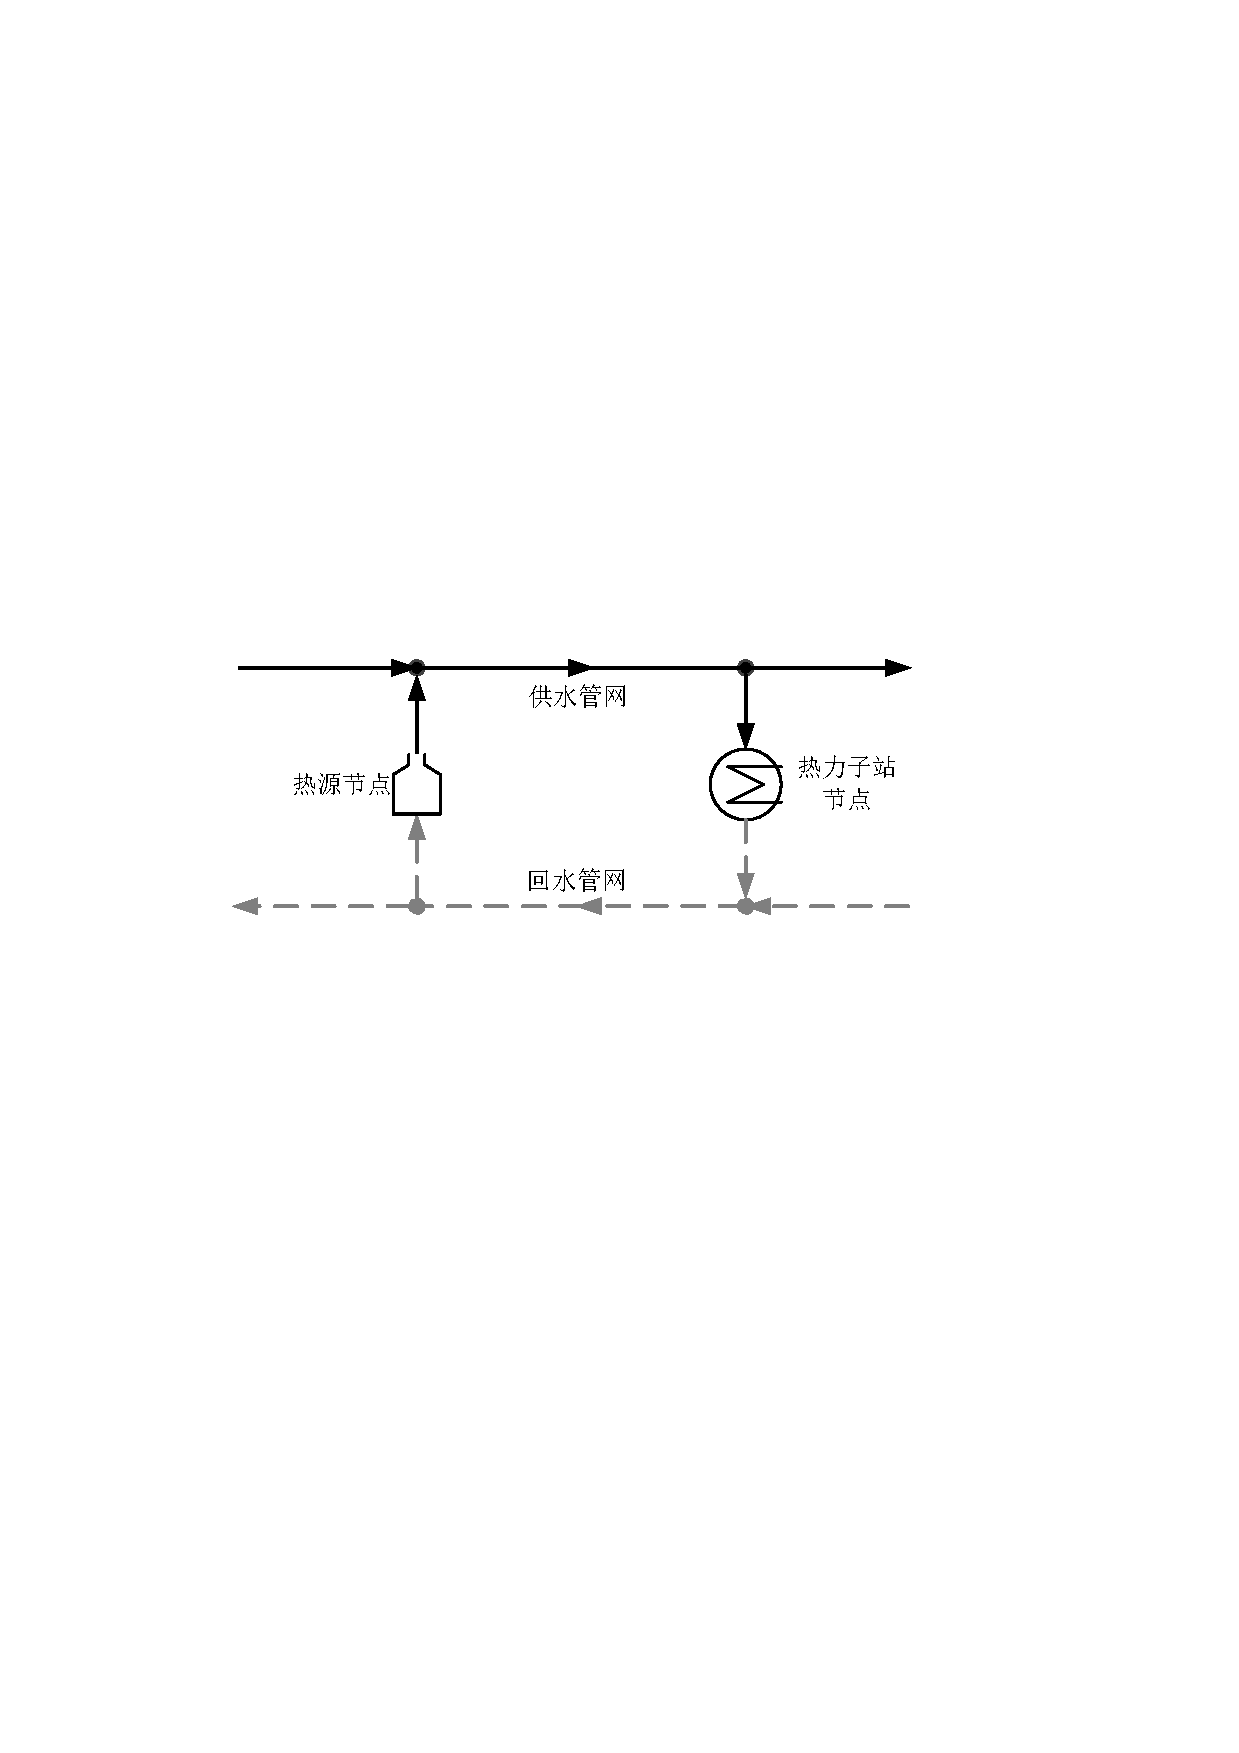
\includegraphics[scale=0.75]{figures/Chap4-3-DHN-Energy-Topo.pdf}
\caption{区域供热网络结构示意图}
\label{Fig:DHN-Topology}
\end{figure}

质量流率(水力分布)可通过质量守恒约束确定\cite{LXZ-DHN-2016, DHN-Model-17},
\begin{subequations}
\label{eq:DHN-Hydra-Part}
\begin{gather}
\sum\limits_{b \in F(i)} {\dot m_{b,t}^S}  + \dot m_{i,t}^d = \dot m_{i,t}^g + \sum\limits_{b \in T(i)} {\dot m_{b,t}^S} ,\forall i,t \label{eq:DHN-Hydra-Part-S}\\
\sum\limits_{b \in F(i)} {\dot m_{b,t}^R}  + \dot m_{i,t}^g = \dot m_{i,t}^d + \sum\limits_{b \in T(i)} {\dot m_{b,t}^R} ,\forall i,t \label{eq:DHN-Hydra-Part-R}\\
0 \le \dot m_{b,t}^S \le \dot m_b^u,0 \le \dot m_{b,t}^R \le \dot m_b^u,\forall b,t\label{eq:DHN-Hydra-Part-Limit}
%\tau^{out} = (\tau^{in}-\tau^{am}){\rm e}^{-\lambda_b l_b/c_p \dot m} + \tau^{am} \label{eq:DHN-Pipe-Loss} \\
%\tau^{mix} = \dfrac{\sum_{b \in L_E(i)} (\tau_b^{out} \dot m_b)}{\sum_{b \in L_E(i)} \dot m_{b}} \label{eq:DHN-Mix-Temp-1} \\
%\tau^{in}_b = \tau^{mix},~ \forall b \in L_B(i)\label{eq:DHN-Mix-Temp-2} \\
%\tau^{out}_b = \tau^{in}_{b'},~ \forall b \in L_E(i),~ \forall b' \in L_B(i)\label{eq:DHN-Mix-Temp-3}
\end{gather}
\end{subequations}
其中,$\dot m_{i,t}^g$与$\dot m_{i,t}^d$分别为节点$i$热源(如AA-CAES能量枢纽)与热负荷的质量流率;$\dot m_b^u$为管道$b$的质量流率上界。(\ref{eq:DHN-Hydra-Part-S})与(\ref{eq:DHN-Hydra-Part-R})分别表示供水侧与回水侧节点$i$的质量平衡约束;(\ref{eq:DHN-Hydra-Part-Limit})表示管道运行的物理限制。

供热网络中热源与热负荷节点的热功率满足,
\begin{subequations}
\label{eq:DHN-heat-power-model}
\begin{gather}
h_{i,t}^{d} = c_p \dot m_{i,t}^d  (\tau_{i,t}^S - \tau_{i,t}^R), \forall i,t \\
h_{j,t}^{hp} = c_p \dot m_{j,t}^g  (\tau_{j,t}^S - \tau_{j,t}^R), \forall j,t \\
h_{i,t}^{g} = c_p \dot m_{i,t}^g  (\tau_{i,t}^S - \tau_{i,t}^R), \forall i,t
\end{gather}
\end{subequations}
%h = c_p \dot m (\tau^S - \tau^R) \label{eq:DHN-Heat-Exchange}\\
其中,$h_{i,t}^d$为热负荷的热功率需求;$h_{j,t}^{hp}$为热泵提供的热功率,且由(\ref{equ:model-HP})决定;$h_{i,t}^g$为其它热源的供热功率。

\subsection{区域配电网络潮流模型}
\label{sec:st-case-dispatch-PDN}
区域供电网络一般为辐射式结构, 如图~\ref{Fig:PDN-Topology}~所示,可采用Dist Flow潮流模型进行建模为\cite{Distflow-WFL, Branchflow-SH1},
\begin{subequations}
\label{eq:PDN-Branch-Flow-All}
\begin{gather}
P_{ij,t} + p_{j,t}^g + W_{j,t}^e - r_{ij}I_{ij,t} = \sum\limits_{k \in \pi(j)} {P_{jk,t}}+ p_{j,t}^d +  W_{j,t}^c + d_{j,t}^{hp},\forall l({i,j}),t \label{eq:PDN-Node-Balance-P}\\
Q_{ij,t} + q_{j,t}^g - x_{ij}I_{ij,t} = \sum\limits_{k \in \pi(j)} {{Q_{jk,t}}}+ q_{j,t}^d,\forall l({i,j}),t \label{eq:PDN-Node-Balance-Q}\\
{U_{j,t}} = {U_{i,t}}-2({{r_{ij}}P_{ij,t} + x_{ij}{Q_{ij,t}}}) + {({{z_{ij}}})^2}{I_{ij,t}},\forall l({i,j}),t \label{eq:PDN-Node-Balance-U}\\
{I_{ij,t}}{U_{i,t}} = {P_{ij,t}}^2 + Q{_{ij,t}^2},\forall l({i,j}),t \label{eq:PDN-Relation-PQ}\\
I_{ij,t} \le I_{ij}^u,U_i^l \le {U_{i,t}} \le U_i^u,\forall i,l({i,j}),t \label{eq:PDN-Limit-UI}\\
p_{i,t}^l \le p_{i,t}^g \le p_i^u,q_i^l \le q_{i,t}^g \le q_i^u,\forall i,t \label{eq:PDN-Limit-PQ}
\end{gather}
\end{subequations}
其中,$P_{ij,t}$与${Q_{ij,t}}$分别为线路的传输有功与无功功率;$p_{j,t}^d$与$q_{j,t}^d$分别为节点$j$的有功与无功功率需求;$p_{j,t}^g$与$q_{j,t}^g$分别为各电源(分布式可再生能源机组、燃气轮机等)有功与无功出力\footnote{文献\inlinecite{CAES-Reactive-18-LGK}指出AA-CAES具有一定的无功支撑能力,本文在此假定其不提供无功,但相关建模分析方法完全适用于考虑其提供无功的场景。};$W_{j,t}^e$,$W_{j,t}^c$,$d_{j,t}^{hp}$分别为I型AA-CAES热电能量枢纽(图
\ref{fig:AA-CAES-Hub-V1})与电网的(电)功率接口;$\pi(j)$ 为节点$j$ 的子节点集合;${x_{ij}},{r_{ij}},{z_{ij}}$ 代表线路电抗、电阻及阻抗;${U_{j,t}}$ 为节点电压幅值$V_{j,t}$的平方;${I_{ij}}$ 为线路电流的平方;上标u与l分别表示上界与下界。(\ref{eq:PDN-Node-Balance-P})与(\ref{eq:PDN-Node-Balance-Q})分别表示节点有功和无功功率平衡方程,若系统中存在风电等其它电源,只需进行相应即可;(\ref{eq:PDN-Node-Balance-U}) 定义节点电压幅值;(\ref{eq:PDN-Relation-PQ})给出线路有功与无功与节点电压及线路电流间的耦合关系;(\ref{eq:PDN-Limit-UI}) 与(\ref{eq:PDN-Limit-PQ})给出各物理量的实际物理限制。

\begin{figure}[H]
\centering
\includegraphics[scale=0.89]{Fig-2-PDN-Topology}
\caption{辐射状配电网结构示意图}
\label{Fig:PDN-Topology}
\end{figure}

Dist Flow模型(\ref{eq:PDN-Branch-Flow-All})描述了热电综合能源系统中的(电功率)潮流分布,其优势在于可以给出节点电压、线路无功等配电网中较为关注的运行信息,同时该模型可被线性化或凸松弛化(如二阶锥松弛\cite{Thesis-Liubin})以高效求解。例如,线性化的DistFlow模型为\cite{BFM-Lin-1,BFM-Lin-2},
\begin{subequations}
\label{eq:Lin-Dist-Flow-Non-OLTC}
\begin{gather}
P_{ij,t} + p_{j,t}^g + W_{j,t}^e = \sum_{k \in \pi(j)} P_{jk,t} + W_{j,t}^c + p_{j,t}^d + d_{j,t}^{hp}, \forall l(i,j),t \label{eq:PF-P} \\
Q_{ij,t} + q_{j,t}^g = \sum_{k \in \pi(j)} Q_{jk,t} + q_{j,t}^d, \forall l(i,j),t \label{eq:PF-Q} \\
U_{j,t} = U_{i,t} - ({r_{ij} P_{ij,t} + x_{ij} Q_{ij,t}}){U_0}, \forall j,t \label{eq:PF-U} \\
U_i^l \le {U_{i,t}} \le U_i^u,\forall i,{U_0} = V_{sl}^2 , \forall i,t \\
p_i^l \le p_{i,t}^g \le p_i^u,q_i^l \le q_{i,t}^g \le q_i^u, \forall i,t
\end{gather}
\end{subequations}
其中,$V_{sl}$为平衡节点的电压幅值,对于辐射状PDN一般为馈入节点的电压幅值。

%特别地,当线路含有离散电容器组进行无功补偿时,(\ref{eq:PF-Q})可修正为
%\begin{equation}
%{Q_{ij,t}} + q_{j,t}^g + \frac{{{U_{j,t}}{C_j}}}{2} + {Q_{cj,t}} - {x_{ij}}{i_{ij,t}} = \sum\limits_{k \in \pi \left( j \right)} {{Q_{jk,t}}}  + q_{j,t}^d,\forall t
%\end{equation}
%
%若配电网中无离散的电容器组等无功补偿装置及OLTC等调节装置时,配电网潮流模型可退化为

对于实际运行的配电网而言,为了维持较好的电压质量,一般会增设连续无功补偿装置(如SVG)、离散的电容器组以及有载调压变压器(OLTC)等。为此,可在线性化DistFlow 模型(\ref{eq:Lin-Dist-Flow-Non-OLTC})的基础上,修正含离散电容器或连续无功补偿装置以及含OLTC线路的无功平衡方程(\ref{eq:PF-Q})与节点电压方程(\ref{eq:PF-U})为\cite{PDN-Model-Reactive-Power-DT-16, CAES-IES-16-Rui},
\begin{subequations}
\label{eq:Lin-Dist-Flow-Plus-OLTC}
\begin{gather}
{Q_{ij,t}} + q_{j,t}^g + \frac{{{U_{j,t}}{C_{j,t}}}}{2} + {q_{j,t}^c} = \sum\limits_{k \in \pi \left( j \right)} {{Q_{jk,t}}}  + q_{j,t}^d,\forall t \label{eq:Lin-Dist-Flow-Plus-OLTC-1}\\
\frac{{{U_{j,t}}}}{{K_{ij,t}^2}} = {U_{i,t}} - \left( {{r_{ij}}{P_{ij,t}} + {x_{ij}}{Q_{ij,t}}} \right)/{U_0},\forall t\label{eq:Lin-Dist-Flow-Plus-OLTC-2}
\end{gather}
\end{subequations}
其中,${C_{j,t}}$为投运的电容或电抗器值; $q_{j,t}^{c}$为连续无功补偿量;$K_{ij,t}^{}$ 为OLTC变比。

\subsection{含~AA-CAES~能量枢纽的热电系统调度模型}

在集中运营模式下,假定无碳排区域热电综合能源系统中的负荷由风电机组与上级电网承担,热能由I型AA-CAES热电能量枢纽提供,系统调度以最小化系统运行成本为目标,即
\begin{subequations}
\label{eq:CAES-Hub-dispatch}
\begin{gather}
\min \;\;\sum\limits_{t \in T} {{\lambda_t}{p_{0,t}^g}} \label{eq:CAES-Hub-dispatch-obj}\\
\mbox{s.t.}~
\mbox{I型AA-CAES能量枢纽热电联供模型}\\
\mbox{PDN线性DistFlow模型}\\
\mbox{供热网络热力-水力潮流模型} \\
W_i^{g,l} \le W_{i,t}^g \le W_i^{g,u},\forall i,t
\end{gather}
\end{subequations}
其中,${\lambda_t}$为电价;${p_{0,t}^g}$为区域热电综合能源系统从上级电网中购入的电功率;$W_{i,t}^g$为风电机组实际出力,$W_i^{g,l}$ 与$W_i^{g,u}$分别为风电出力最小值与预测值。

无碳排调度模型(\ref{eq:CAES-Hub-dispatch})为非线性优化问题,其非线性主要源自配电网潮流模型及供热网络潮流模型,本小节将分别给出相应的线性化方法,以在不丢失准确性的同时将模型转化为易于高效求解的MILP问题。事实上,OLTC、电容/电抗器组等离散型无功补偿装置的调节或投切亦存在相应的运行成本,目标函数(\ref{eq:CAES-Hub-dispatch-obj})中可进一步扩展至考虑无功补偿成本,相关的线性化及求解方法也基本适用。

\subsubsection{配电网潮流模型的线性化}
改进的区域配电网潮流模型(\ref{eq:Lin-Dist-Flow-Non-OLTC})-(\ref{eq:Lin-Dist-Flow-Plus-OLTC}) 中的非线性主要源自离散电容器组引起的非线性项${U_{j,t}}{C_j}/2$与OLTC变比调节引入的非线性项${{{U_{j,t}}}}/{{K_{ij,t}^2}}$。类似于\ref{sec:chap3-bid-aa-caes}节中的布尔展开法,非线性项${U_{j,t}}{C_j}/2$中的离散量$C_j$可线性化为\cite{PDN-Model-Reactive-Power-DT-16, CAES-IES-16-Rui},
\begin{subequations}
\begin{gather}
\label{eq:UC-approx}
{{C_j} = C_j^l + {s_j}({{2^0}{g_{j,0}} + {2^1}{g_{j,1}} + \cdots + {2^{{v_j}}}{g_{j,{v_j}}}})}, {{g_{j,0}},{g_{j,1}}, \cdots ,{g_{j,{v_j}}} \in \{ 0,1\} }\\
{0 \le {2^0}{g_{j,0}} + {2^1}{g_{j,1}} +  \cdots  + {2^{{v_j}}}{g_{j,{v_j}}} \le ({C_j^u - C_j^l})/{s_j},}{\forall j \in {E_D}}
\end{gather}
\end{subequations}
其中,$C_j^l$与$C_j^u$分别为电容器或电抗器容量的最小值与最大值;${s_j}$ 为电容器或电抗器的步进容量;${E_D}$ 为增设电容器或电抗器的母线集合;整数变量$v_j$ 表征离散化段数,可由下式决定
\begin{equation}
{\log _2}({\frac{{C_j^u - C_j^l}}{{{s_j}}} + 1})-1 \le {v_j} \le {\log _2}({\frac{{C_j^u - C_j^l}}{{{s_j}}} + 1})
\end{equation}
因此,非线性项${U_{j,t}}{C_{j,t}}$可转化为,
\begin{equation}
\label{eq:UC-approx-2}
{U_{j,t}}{C_{j,t}} = C_j^l{U_{j,t}} + {s_j}({{2^0}{\delta _{j,0}} +  \cdots  + {2^{{v_j}}}{\delta _{j,{v_j}}}})
\end{equation}
进一步,式(\ref{eq:UC-approx-2})可用大M法\cite{Big-M-1981} 线性化,即
\begin{subequations}
\label{eq:UC-approx-final}
\begin{gather}
%{{U_{j,t}}{C_{j,t}} = C_j^l{U_{j,t}} + {s_j}\left( {{2^0}{\delta _{j,0}} +  \cdots  + {2^{{v_j}}}{\delta _{j,{v_j}}}} \right)}\\
{{U_{j,t}} - M({1 - {g_{j,k,t}}}) \le {\delta _{j,k,t}} \le {U_{j,t}} + M({1 - {g_{j,k,t}}})}\\
{ - M{g_{j,k,t}} \le {\delta _{j,k,t}} \le M{g_{j,k,t}}}
\end{gather}
\end{subequations}
其中,${\delta _{j,k,t}}$为辅助的连续量;M为一足够大的正数。

针对含有载调压器~OLTC~的支路~$l(i,j)$,其无功功率约束(\ref{eq:Lin-Dist-Flow-Plus-OLTC-2})可线性化为,
\begin{equation}
\label{eq:OLTC-approxi-1}
\frac{{{U_{j,t}}}}{{K_{ij,t}^2}} = {U_{j,t}}({\frac{{{b_{ij,1,t}}}}{{K_{ij,1}^2}} + \frac{{{b_{ij,2,t}}}}{{K_{ij,2}^2}}{\rm{ + }} \cdots {\rm{ + }}\frac{{{b_{ij,{n_{ij}},t}}}}{{K_{ij,{n_{ij}}}^2}}})
\end{equation}
其中,$K_{ij,1}^{}$, $K_{ij,2}^{}$, ..., $K_{ij,{n_{ij}}}^{}$ 为增设于线路$l(i,j)$ 的OLTC变比的可能取值;${n_{ij}}$为相应的变比离散取值个数。

综上,含OLTC的节点电压约束(\ref{eq:Lin-Dist-Flow-Plus-OLTC-2})可线性化为\cite{PDN-Model-Reactive-Power-14, PDN-Model-Reactive-Power-DT-16, CAES-IES-16-Rui},
\begin{subequations}
\label{eq:OLTC-approxi-2}
\begin{gather}
{{U_{j,t}}/K_{ij,t}^2 = \sum\limits_{k = 1}^{{n_{ij}}} {{h_{j,k,t}}/K_{ij,k}^2} }\\
{{b_{ij,1,t}}, \cdots ,{b_{ij,{n_{ij}},t}} \in \{ 0,1\} ,\sum\limits_{k = 1}^{{n_{ij}}} {{b_{j,k,t}}}  = 1}\\
{ - M({1 - {b_{ij,k,t}}}) + {U_{j,t}} \le {h_{j,k,t}} \le M({1 - {b_{ij,k,t}}}) + {U_{j,t}}}\\
{ - M{b_{ij,k,t}} \le {h_{j,k,t}} \le M{b_{ij,k,t}}}
\end{gather}
\end{subequations}
其中,$h_{j,k,t}$为辅助的连续变量。

\subsubsection{区域热网潮流模型的线性化}
%热网模型(\ref{eq:DHN-Thermal-Part})-(\ref{eq:DHN-Hydra-Part})采用耦合的水力和热力模型描述热网中工质的水力工况(压强、质量流率)和热力工况(供回水温度), 模型较为复杂。

区域供热网络存在两种调节方式,即CF-VT与VF-VT\cite{DHN-CFVT-2013},前者通过固定质量流率调节供(回)水温度来满足供热负荷随外界温度的变化需求,而后者通过质量流率和供(回)水温度的共同调节来满足日供热负荷需求。

由(\ref{eq:DHN-heat-power-model})可知,当日供热负荷波动范围较大时,仅靠温度的调节往往不能满足供热负荷需求,加之供热管道温度半动态的存在导致温度调节的响应存在时延\cite{IES-DHN-16-LZG},调节灵活性与及时性往往不高。因此,CF-VT模式存在一定局限性。质量流率调节响应速度快,可为供热负荷的调节带来更高的灵活性,使得VF-VT 模式具备更大的灵活性。然而,VF-VT 模式下水力工况和热力工况耦合性强,模型求解较为困难。实际运行中一般先计算水力分布,确定工质质量流率,进而进行CF-VT 调节。因此,我们假定日内热负荷的调整仅通过CF-VT模式实现,即$\dot m$已知,从而非线性模型(\ref{eq:DHN-Thermal-Part})(\ref{eq:DHN-Hydra-Part})退化为线性模型。

\subsection{集中运营热电综合能源系统算例分析}
本小节分析含图~\ref{fig:AA-CAES-Hub-V1}所示的I型~AA-CAES~ 能量枢纽的零碳排区域热电综合能源系统的最优调度。算例中的仿真由配有i5-4210M CPU 与16 GB RAM 的计算单元完成,模型采用YALMIP\cite{YALMIP}建模,求解器为CPLEX\footnote{具体代码可参见https://github.com/AIRicky/Integrated-Energy-Systems-with-CAES}。

\subsubsection{算例设置}
采用图\ref{Fig:Hub-Dispatch-Exe-PDN33DHN8}所示的测试系统模拟园区级或区域级无碳排热电综合能源系统,该系统由33节点PDN、8节点DHN、I型AA-CAES能量枢纽、4台风机组成。母线2处含一座容量为3MW(6台0.5MW风机组成)的小型风电场,其它母线处的风机容量均为0.5MW。

\begin{figure}[H]
\centering
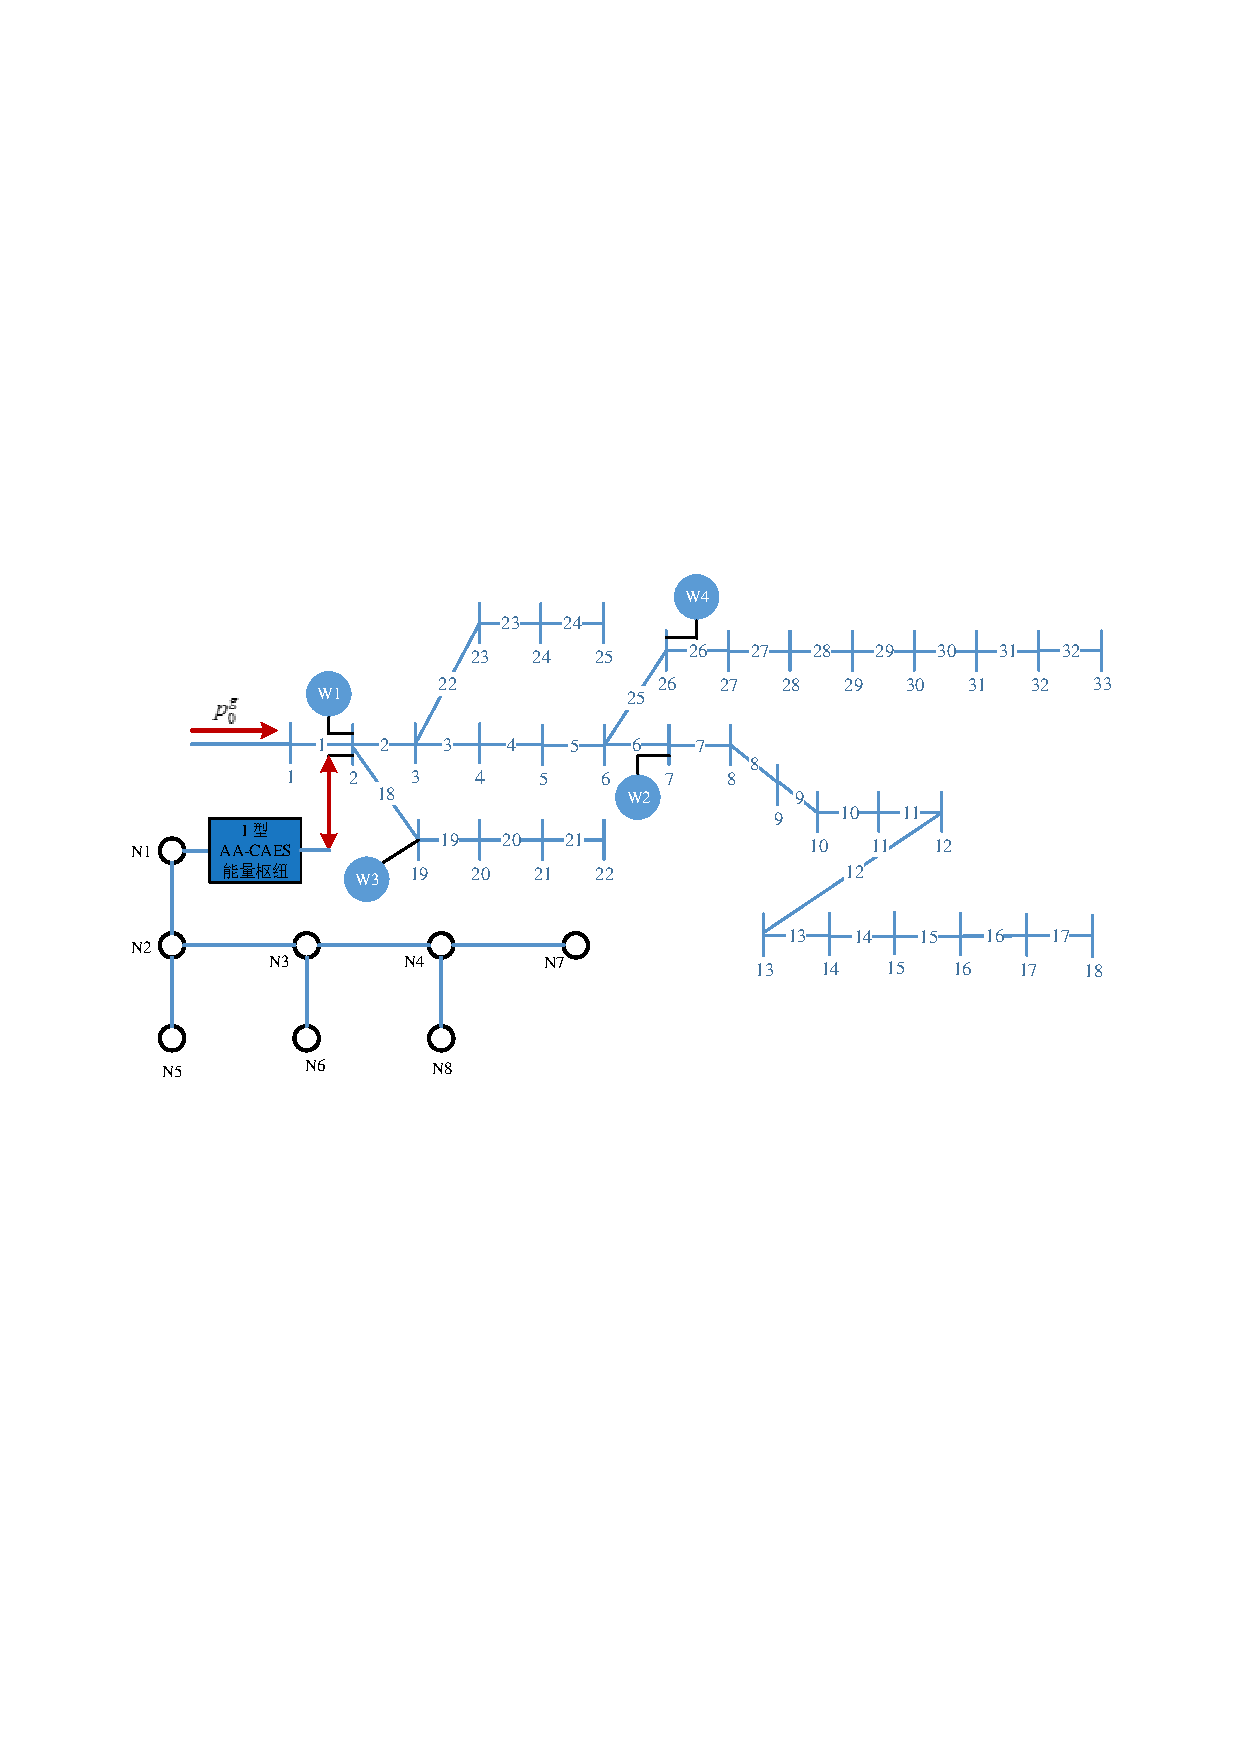
\includegraphics[scale=0.80]{figures/Chap4-15-Hub-Dispatch-Exe-PDN33DHN8-V2.pdf}
\caption{集中运营环境下的区域热电综合能源测试系统}
\label{Fig:Hub-Dispatch-Exe-PDN33DHN8}
\end{figure}

\begin{figure}[H]
\centering
\includegraphics[scale=0.60]{figures/Chap4-15-Hub-Dispatch-Exe-TOU.pdf}
\caption{分时电价曲线}
\label{Fig:Hub-Dispatch-Exe-TOU}
\end{figure}

鉴于该类无碳排园区级热电综合能源系统在我国较为常见,此处采用图~\ref{Fig:Hub-Dispatch-Exe-TOU}所示的电力市场分时电价曲线。对于实时电价等美国电力批发市场较为常见的价格机制,我们将在第~\ref{sec:bid-st-caes}节独立运营模式下的AA-CAES能量枢纽的市场竞标问题中进行讨论。系统中所有风电机组的总功率预测曲线(各风机按容量分配)、总电负荷及热负荷需求如图~\ref{Fig:Hub-Dispatch-Exe-PQWHG} 所示,电网各母线负荷分配比例由MATPOWER 33 节点配电网标准潮流~\cite{MATPOWER} 求得, 热网各节点热负荷分配比例及质量流率见表\ref{tab:para-thermo-load}。

\begin{figure}[H]
\centering
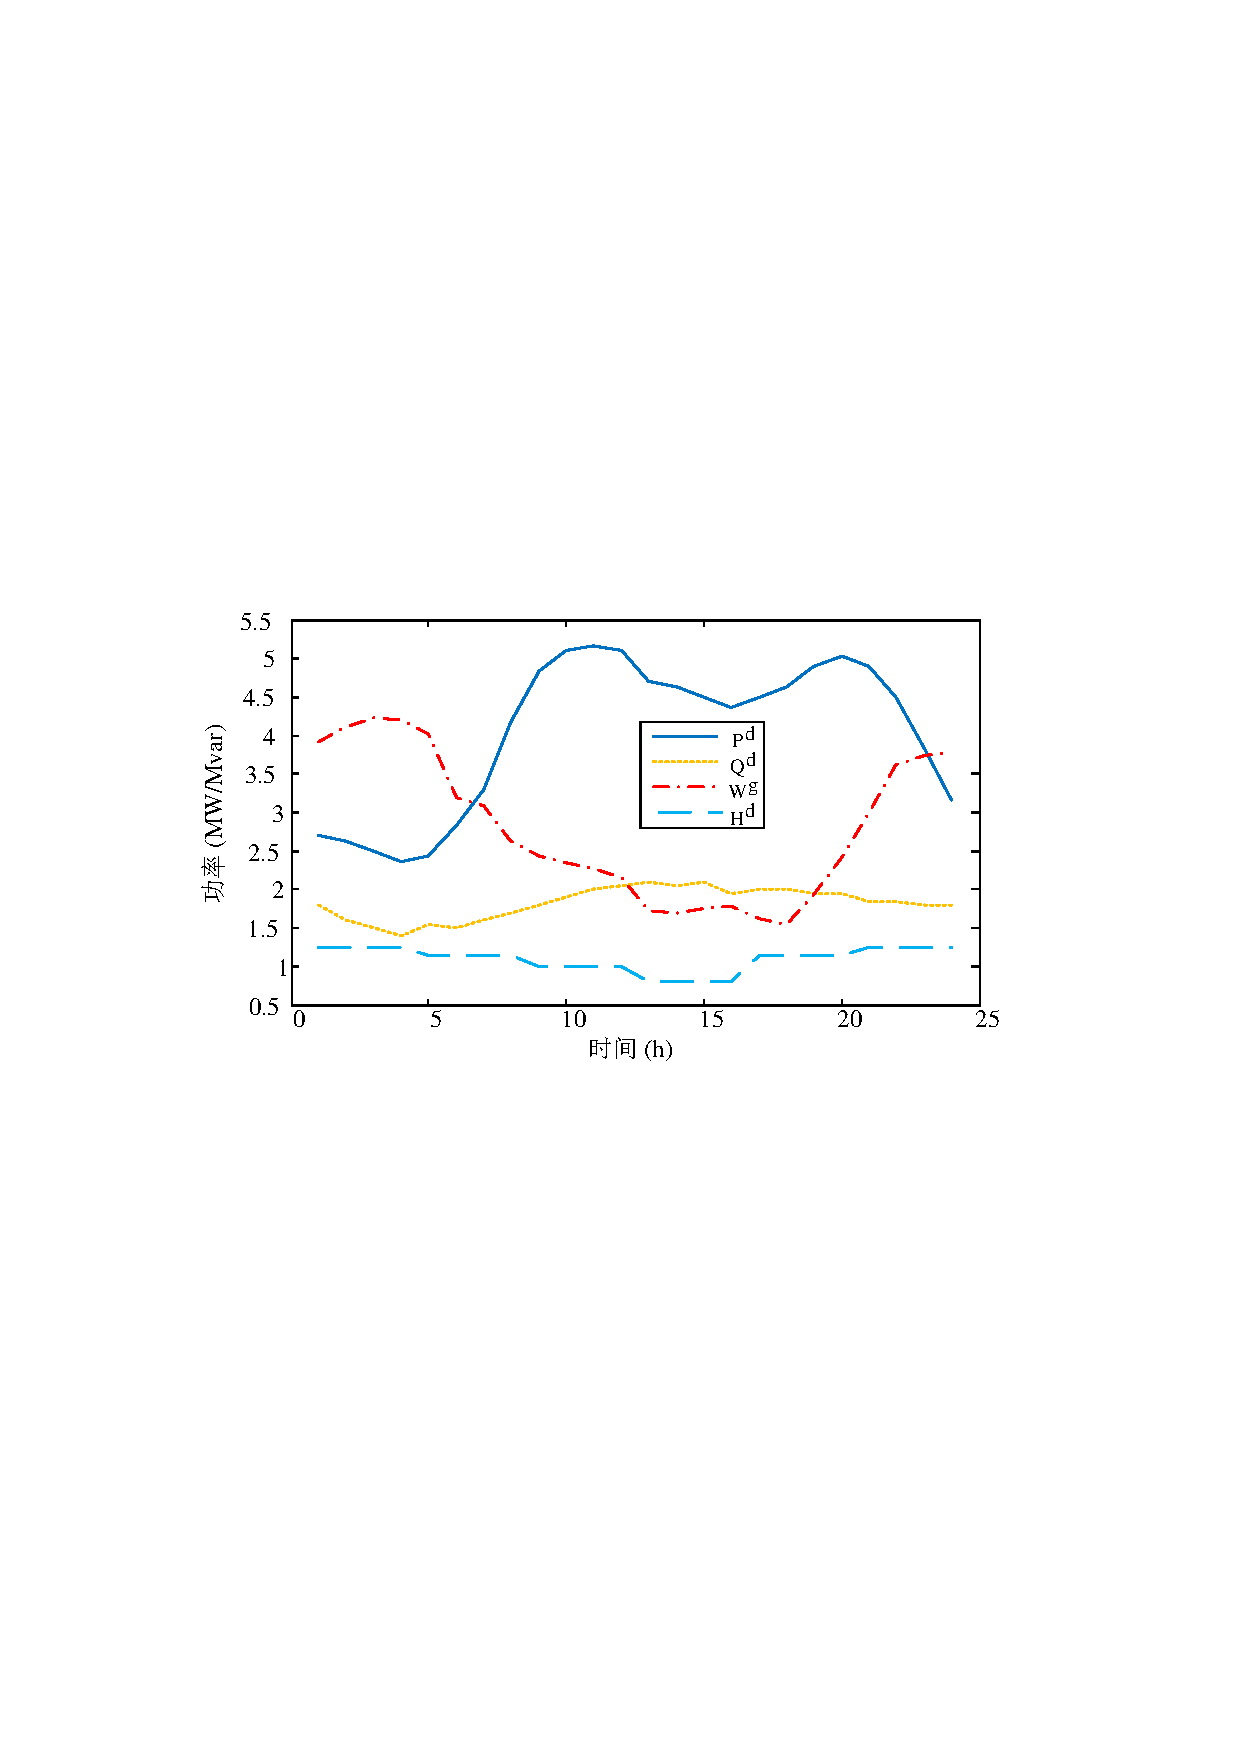
\includegraphics[scale=0.81]{figures/Chap4-15-Hub-Dispatch-Exe-PQWHG.pdf}
\caption{负荷需求与风电预测功率}
\label{Fig:Hub-Dispatch-Exe-PQWHG}
\end{figure}

\begin{table}[htb]
  \centering
  \begin{minipage}[t]{0.65\linewidth} % 如果想在表格中使用脚注,minipage是个不错的办法
  \caption{8节点区域热网节点参数}
  \label{tab:para-thermo-load}
    \begin{tabularx}{\linewidth}{ccccccccc}
      \toprule[1.5pt]
      {\heiti 节点编号} & {\heiti \#1} & {\heiti \#2} &  {\heiti \#3} & {\heiti \#4} & {\heiti \#5} & {\heiti \#6} & {\heiti \#7} & {\heiti \#8} \\\midrule[1pt]
      负荷比例 (\%)& 0  & 0 & 0	& 0	& 20 & 20 & 20 & 40\\
      质量流率 (kg/s)& 10	& 0	& 0	& 0	& 2	  & 2   & 2	  & 4\\
      \bottomrule[1.5pt]
    \end{tabularx}
  \end{minipage}
\end{table}

为了维持配电网中各母线的电压质量,在配电网各中枢节点部署了无功补偿装置。参考文献\inlinecite{Thesis-Liubin}中的系统设置,在线路\#1, \#18, \#22, \#25 上装设最小分接头为0.95,最大分接头为1.05 以及分接头步长为0.01的OLTC\cite{Thesis-Liubin}。并联电容器装设于母线 \#5, \#10, \#13, \#17, \#20, \#23, \#30,其容量范围为0-0.2,调节步长为~0.05。此外,SVG增设于母线~\#4, \#9, \#14,以提供连续无功补偿。

\subsubsection{能量枢纽仿真}
本小节先仿真分析I型能量枢纽内部的AA-CAES在一个循环周期内的能量平衡情况,为分析其在热电综合能源系统中的供能特性提供参考。内置的AA-CAES采用两级压缩两级膨胀结构,采用常压-常压运行方式及热电联供供能模式,储气库的工作压力范围为8.4 MPa-9.0 MPa。由于常压-常压运行模式的设定,储气库的压力变化对压缩机与膨胀机的部分负载运行影响不大。同时,储气库的压力工作范围较窄,温度变化也不大。压缩机与膨胀机的额定质量流率分别为0.64 kg/s, 2.46 kg/s,其它参数分别如表\ref{tab:para-comp-energy-hub-dispatch}及表\ref{tab:para-turb-energy-hub-dispatch}所示,储气库体积为 2000 m$^3$。

\begin{table}[htb]
  \centering
  \begin{minipage}[t]{0.85\linewidth} % 如果想在表格中使用脚注,minipage是个不错的办法
  \caption{压缩机额定参数}
  \label{tab:para-comp-energy-hub-dispatch}
    \begin{tabularx}{\linewidth}{ccccccc}
      \toprule[1.5pt]
      {\heiti 级数} &  {\heiti 进口压力 } & {\heiti 出口压力} & 进口温度 &  出口温度 & 额定功率 & 等熵效率 \\\midrule[1pt]
       一级  & 0.1 MPa  & 1.15 MPa & 15	$^\circ$C & 375 $^\circ$C &	250 kW & 0.85 \\
       二级  & 1.15 MPa & 9	 MPa  & 40 $^\circ$C  & 366 $^\circ$C & 250 kW & 0.81 \\
      \bottomrule[1.5pt]
    \end{tabularx}
  \end{minipage}
\end{table}

\begin{table}[htb]
  \centering
  \begin{minipage}[t]{0.85\linewidth} % 如果想在表格中使用脚注,minipage是个不错的办法
  \caption{膨胀机额定参数}
  \label{tab:para-turb-energy-hub-dispatch}
    \begin{tabularx}{\linewidth}{ccccccc}
      \toprule[1.5pt]
      {\heiti 级数} &  {\heiti 进口压力} & {\heiti 出口压力} & 进口温度 &  出口温度 & 额定功率 & 等熵效率 \\\midrule[1pt]
      一级  & 8.4 MPa  & 0.94 MPa & 280 $^\circ$C & 60 $^\circ$C  & 500 kW & 0.82 \\
      二级  & 0.94 MPa & 1 MPa    & 280 $^\circ$C & 60 $^\circ$C  & 500 kW & 0.82 \\
      \bottomrule[1.5pt]
    \end{tabularx}
  \end{minipage}
\end{table}

在上述设定下,基于第\ref{cha:simulation}章热力学仿真模型得出一个循环周期内I型能量枢纽内部AA-CAES的能量平衡如图~\ref{Fig:Hub-Dispatch-AA-CAES-Flow}所示,其电-电转换效率为${\eta _{elec}}$ = 1.46/2.8 = 52.14\%,热效率为$\eta_{heat}$=0.4193/2.8=14.98\%,(热电)总能利用效率为${\eta _{total}}$ =(1.46 + 0.4193)/2.8 = 67.12\%。在合适的电力市场环境下, 该效率值对于AA-CAES 型能量枢纽的商业化运行是可接受的。

\begin{figure}[H]
\centering
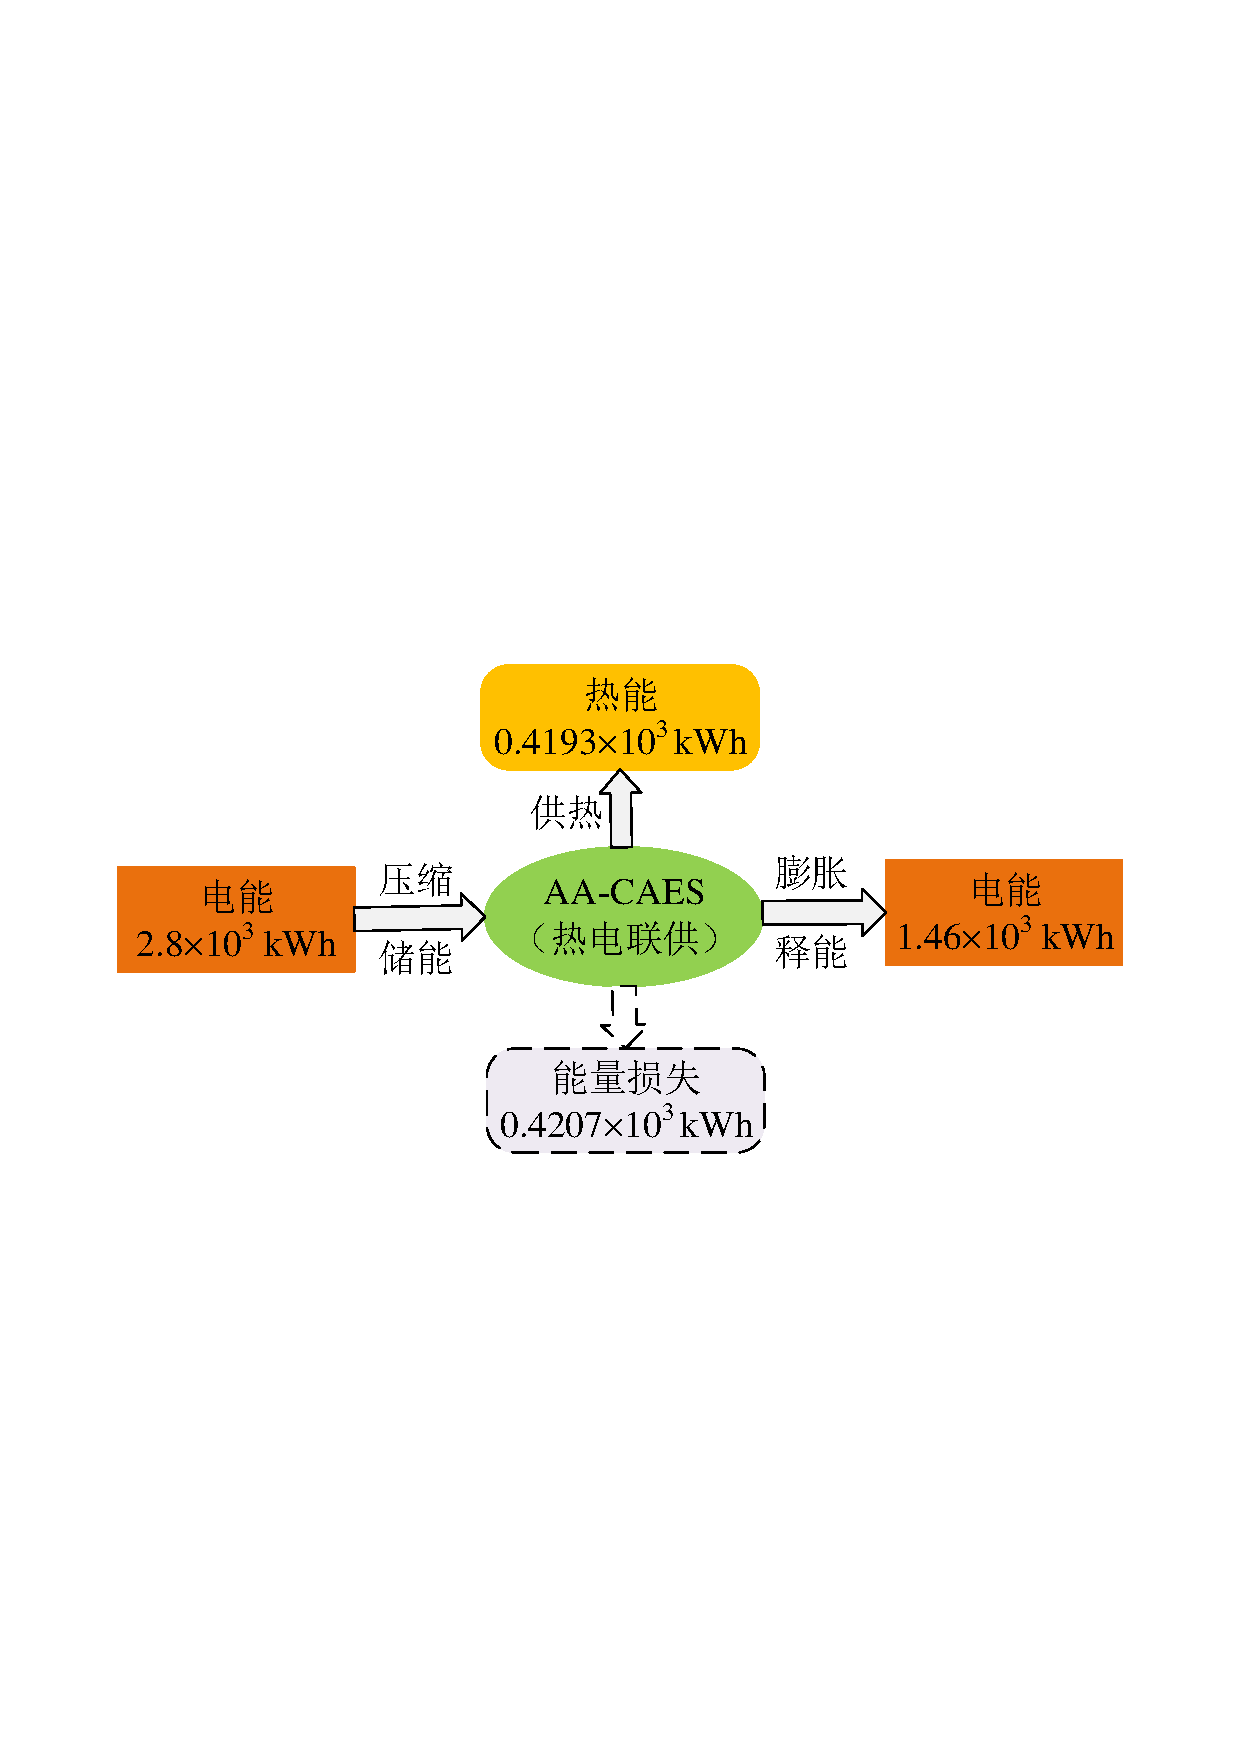
\includegraphics[scale=0.65]{figures/Chap4-15-Hub-Dispatch-AA-CAES-Flow-V2.pdf}
\caption{AA-CAES在一个循环周期内的能量平衡}
\label{Fig:Hub-Dispatch-AA-CAES-Flow}
\end{figure}

\subsubsection{结果分析}

(1)AA-CAES能量枢纽

AA-CAES热电多能联供时,储气库储气压力的变化仅由压缩储能消耗与膨胀释能输出的电功率有关,而储热罐中的储热水平不仅与压缩功率及膨胀功率有关,还与当前的供热功率有关。I型能量枢纽中AA-CAES的储气水平与储热水平变化曲线分别如图~\ref{Fig:Hub-Dispatch-Exe-ASU-SOC} 及\ref{Fig:Hub-Dispatch-Exe-TES-SOC}所示。

\begin{figure}[H]
\centering
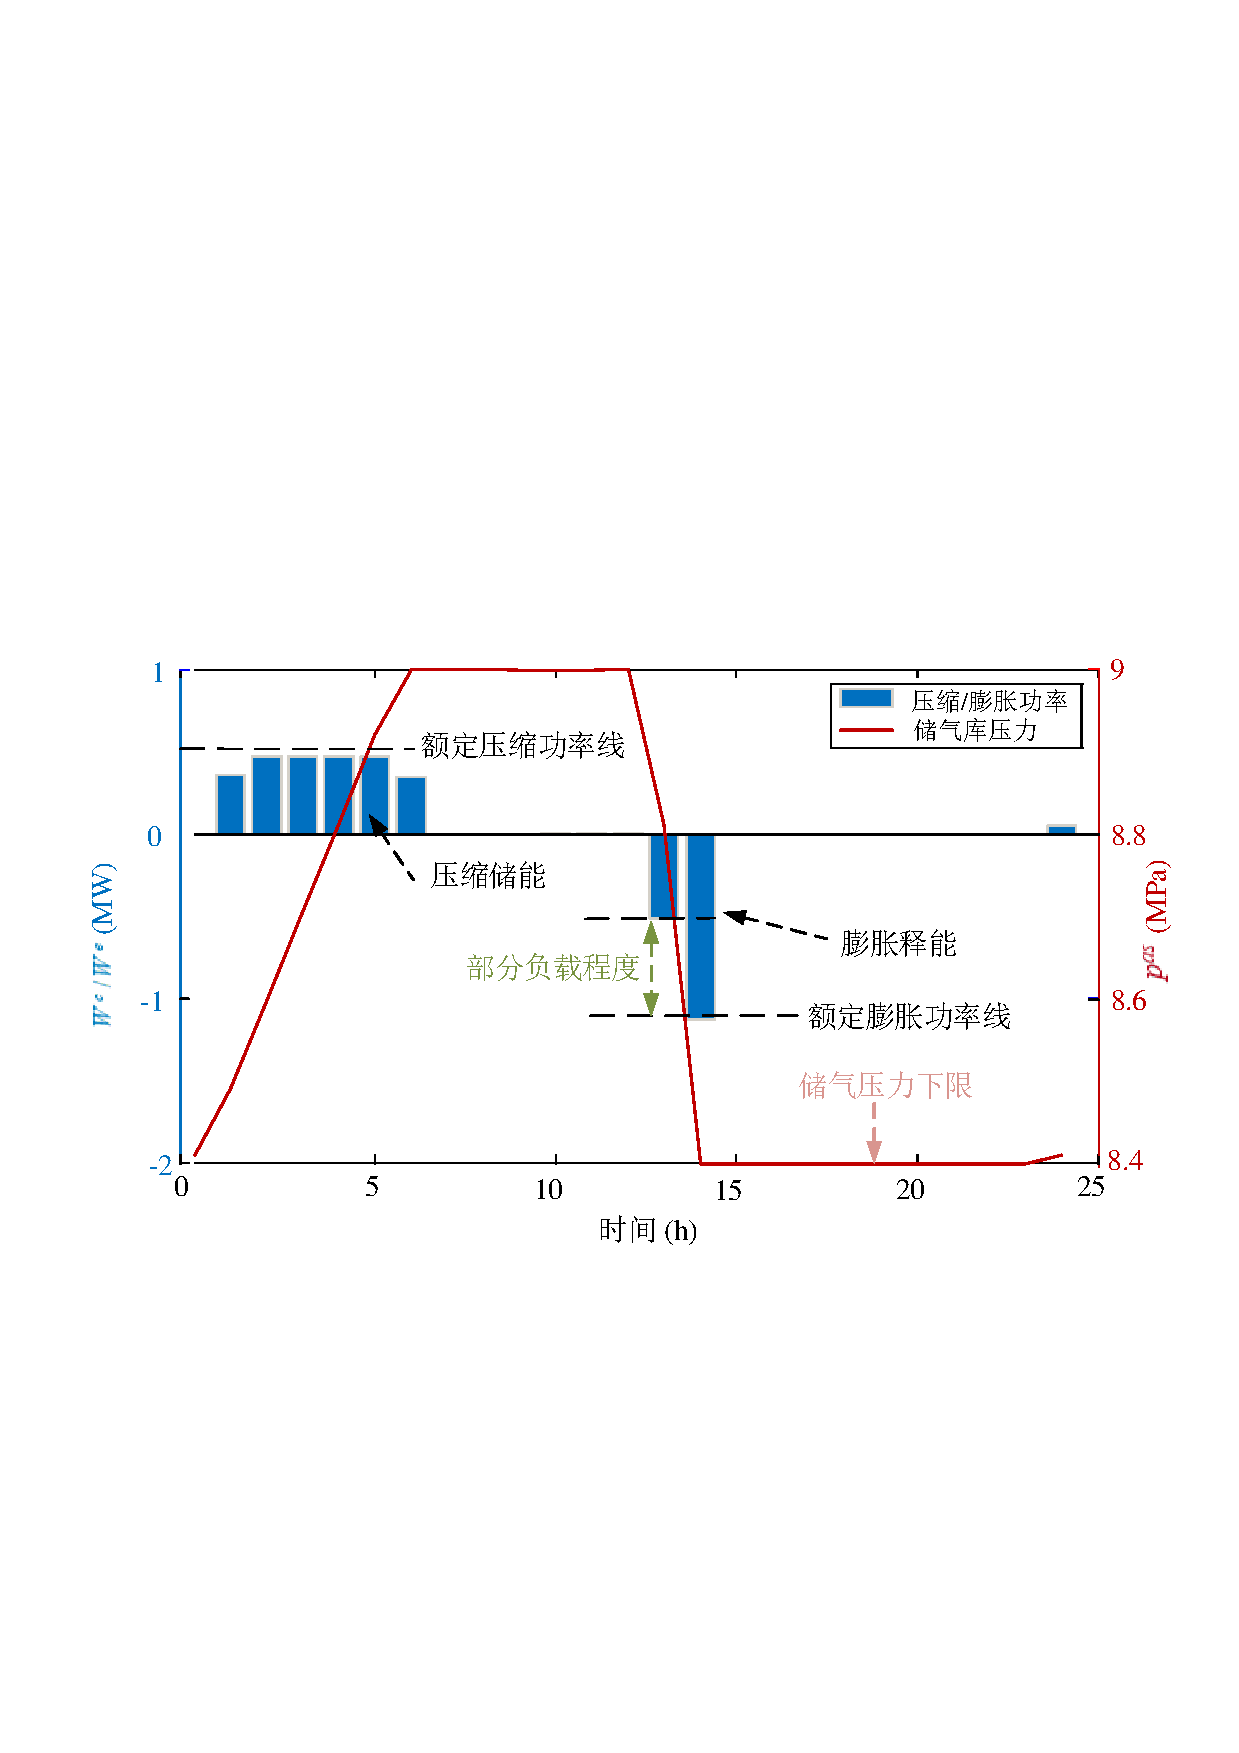
\includegraphics[scale=0.66]{figures/Chap4-15-Hub-Dispatch-Exe-ASU-SOC-V2.pdf}
\caption{AA-CAES能量枢纽储气水平曲线}
\label{Fig:Hub-Dispatch-Exe-ASU-SOC}
\end{figure}

\begin{figure}[H]
\centering
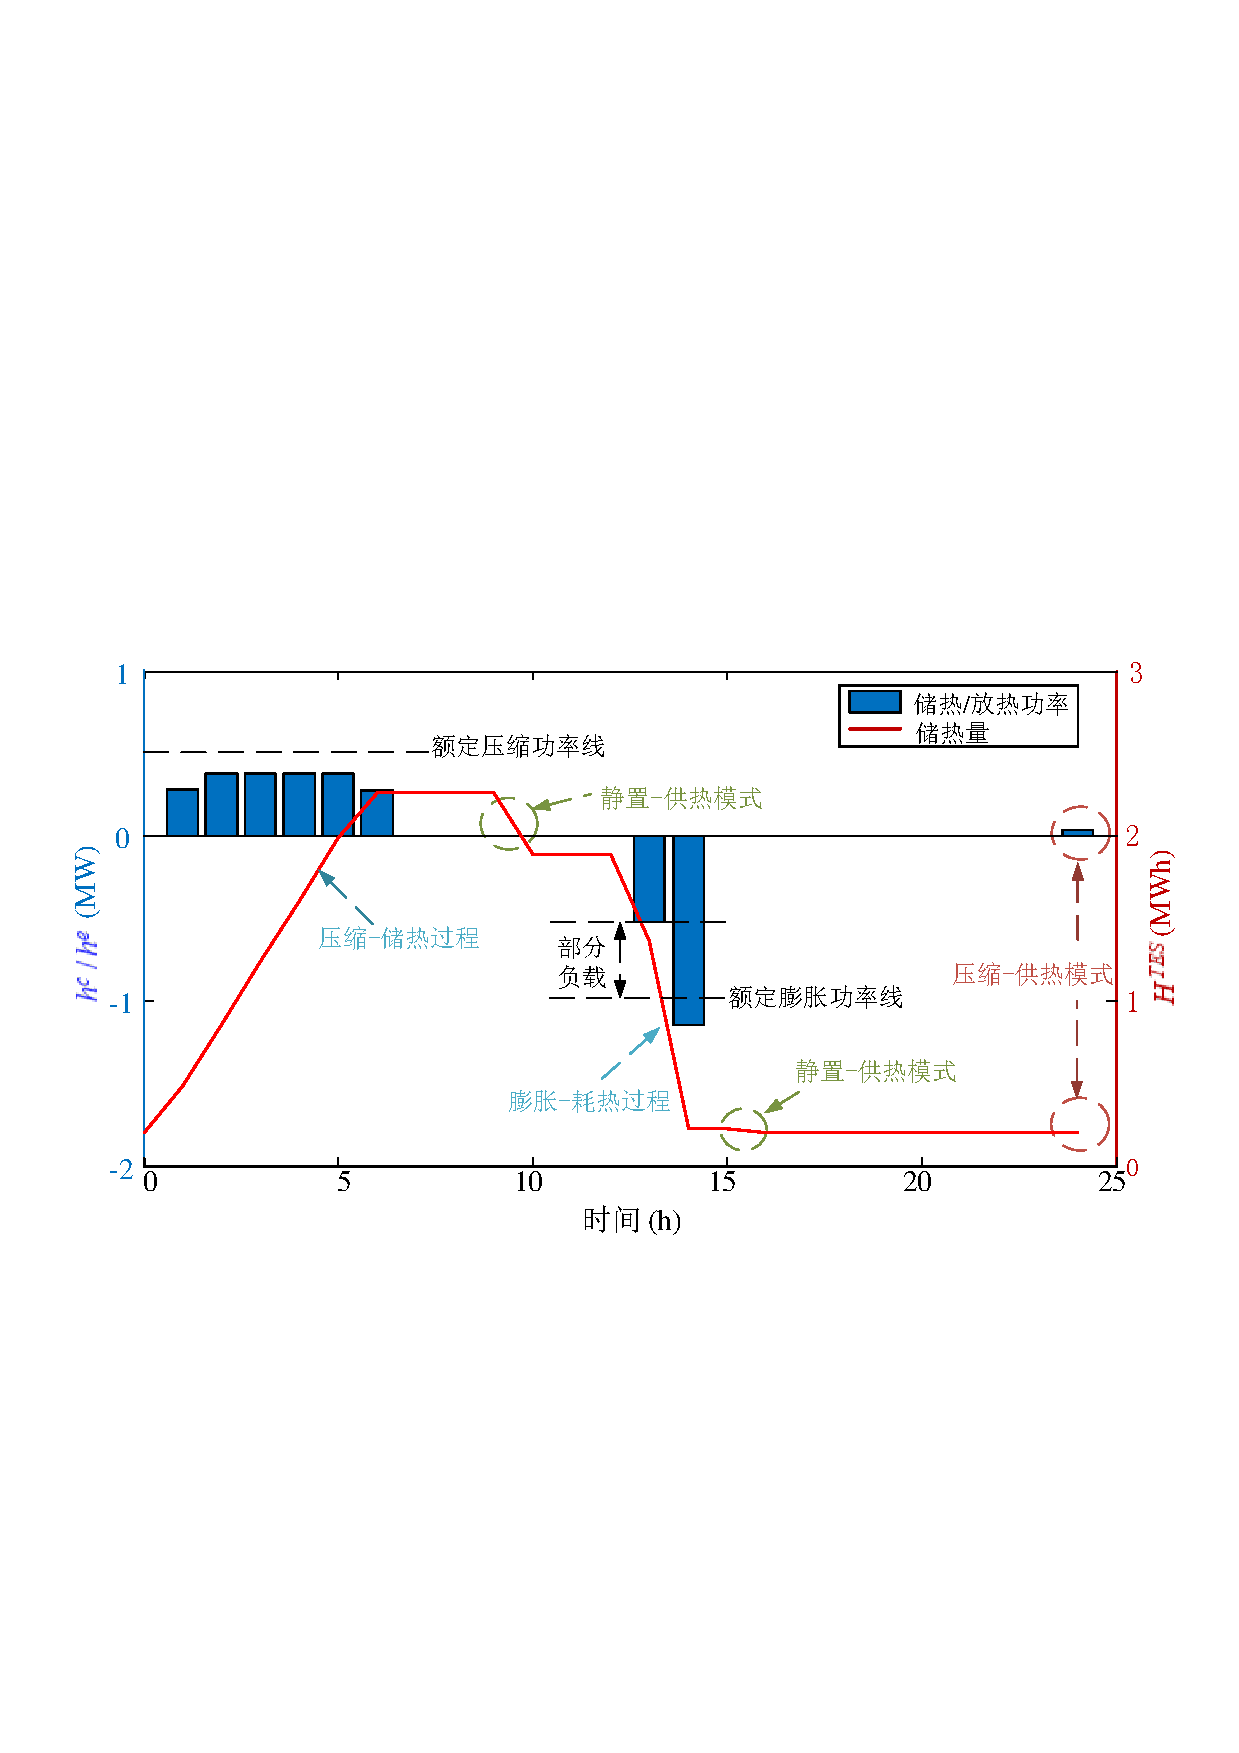
\includegraphics[scale=0.65]{figures/Chap4-15-Hub-Dispatch-Exe-TES-SOC-V2.pdf}
\caption{AA-CAES能量枢纽储热水平曲线}
\label{Fig:Hub-Dispatch-Exe-TES-SOC}
\end{figure}

I型能量枢纽中AA-CAES在多能联供模式下具有的供能灵活性,使其既可以经典的压缩-储热模式(时段1-时段6)与膨胀-耗热模式(时段13-时段14)运行,以实现电能“缓存”与“搬移”,又可运行于静置-供热模式(时段10、时段16)与压缩-供热模式(时段24),从而为区域热电综合能源系统注入运行灵活性。在当前的系统设定下,压缩机可以实现高负载或额定功率运行来减小购电成本,而膨胀机则在部分时段(时段13)以部分负载方式发电,消耗低谷时段存储的低价电能,以降低热电综合能源系统总体运行成本。

此外,由图~\ref{Fig:Hub-Dispatch-Exe-ASU-SOC}及图\ref{Fig:Hub-Dispatch-Exe-TES-SOC}可以看出,实际调度运行时AA-CAES损失能量较多。结合图
\ref{Fig:Hub-Dispatch-AA-CAES-Flow}可知,AA-CAES在一个循环周期存在32.88\%的能量损失,而该损失主要源自储气库入口节流阀与出口节流阀实现的常压-常压运行模式带来的节流损失。事实上,可由压缩机与膨胀机适当地运行于由背压变化及入口压力变化引起的部分负载工况,便可减小由入口与出口节流阀带来的损失。

\begin{figure}[H]
\centering
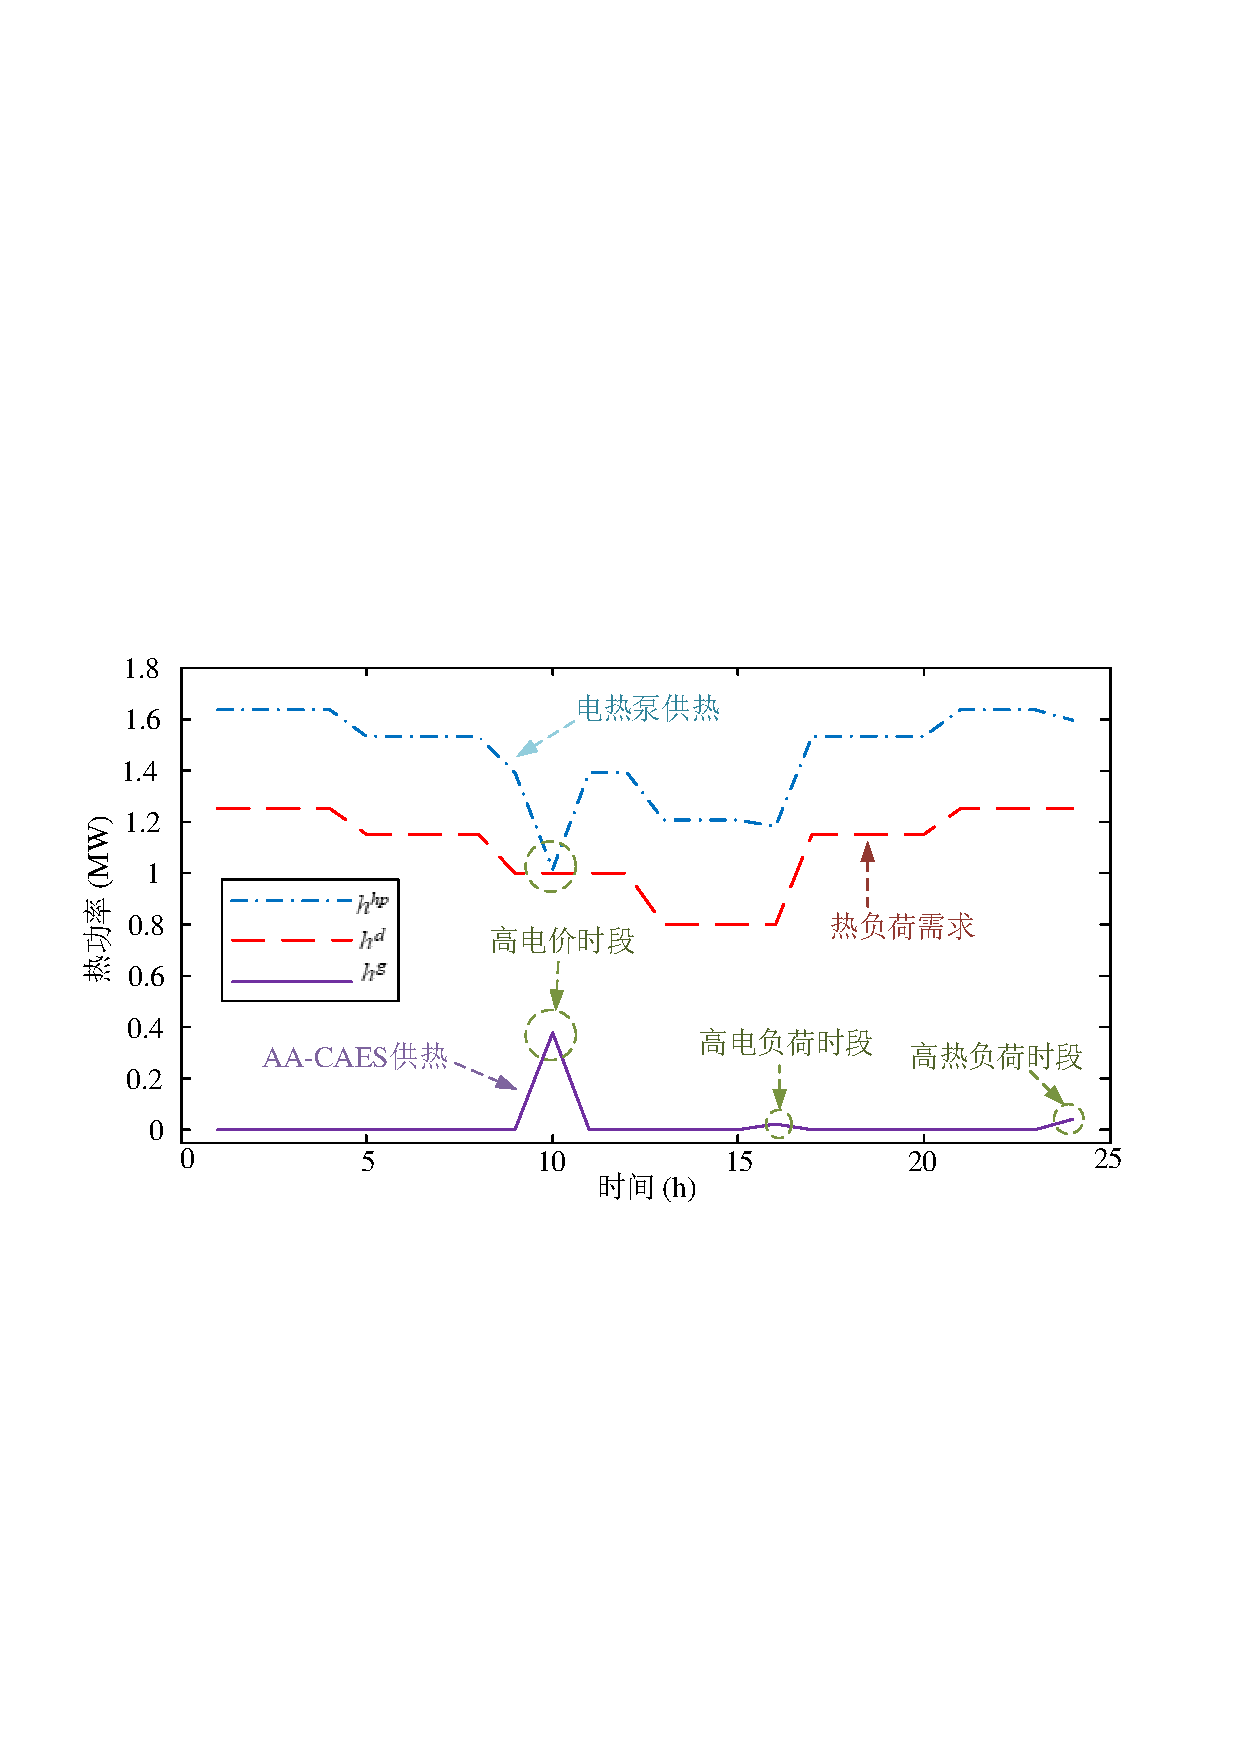
\includegraphics[scale=0.70]{figures/Chap4-15-Hub-Dispatch-Exe-H-gen-V2.pdf}
\caption{热泵与AA-CAES热功率输出曲线}
\label{Fig:Hub-Dispatch-Exe-H-gen}
\end{figure}

I型能量枢纽中热泵与AA-CAES的热功率分配如图~\ref{Fig:Hub-Dispatch-Exe-H-gen}所示,电热泵由于电热转换效率高,承担了系统的大部分热负荷,但由于其不具备热能的缓冲作用,在高峰电负荷及高电价时段其供热成本较高。I型能量枢纽中AA-CAES具有电能及热能的缓冲作用,使其可与电热泵匹配实现能量枢纽的经济运行。AA-CAES 在非(用电)高峰期利用风电和廉价电力运行于压缩储能模式(时段1到时段6),并以储热罐中的热能和储气罐中的压力势能两种形式解耦存储电能;系统电负荷需求较高时,AA-CAES 运行于膨胀释能模式(时段13、时段14),消耗存储在储热罐中的部分热能,并利用储气罐中的空气势能进行发电。伴随AA-CAES压缩储能模式存储的部分(富余)热能,可在电价较高时段(如时段10,见图\ref{Fig:Hub-Dispatch-Exe-TOU})、热负荷需求较高时段(时段24,见图\ref{Fig:Hub-Dispatch-Exe-PQWHG})为系统提供热能,以代替该时段经济性较差的电热泵,同时也可在电负荷需求较高时段(时段16,见图\ref{Fig:Hub-Dispatch-Exe-PQWHG})可为系统提供热能,以降低电热泵为供热消耗电能给配电网带来的调峰压力。

(2)运行成本及弃风量

在考虑与不考虑AA-CAES能量枢纽的两种情况下,图\ref{Fig:Hub-Dispatch-Exe-PDN33DHN8}所示的热电综合能源系统中风电实际输出功率、上级电网的购电功率及母线\#2处风机的弃风分别如图~\ref{Fig:Hub-Dispatch-Exe-Wind-Cur-MEI}及图~\ref{Fig:Hub-Dispatch-Exe-Wind-Curt-PDN} 所示。

\begin{figure}[H]
\centering
\includegraphics[scale=0.65]{figures/Chap4-15-Hub-Dispatch-Exe-Wind-Cur-MEI-V2.pdf}
\caption{考虑能量枢纽时的系统电功率平衡}
\label{Fig:Hub-Dispatch-Exe-Wind-Cur-MEI}
\end{figure}

\begin{figure}[H]
\centering
\includegraphics[scale=0.62]{figures/Chap4-15-Hub-Dispatch-Exe-Wind-Curt-PDN-V3.pdf}
\caption{不考虑能量枢纽时的系统电功率平衡}
\label{Fig:Hub-Dispatch-Exe-Wind-Curt-PDN}
\end{figure}

对比图~\ref{Fig:Hub-Dispatch-Exe-Wind-Cur-MEI}及\ref{Fig:Hub-Dispatch-Exe-Wind-Curt-PDN}可以得出,从时段8至时段22,由于电力负荷需求较高,所有风电均用于供应负荷,该综合能源系统的弃风主要发生在低谷时段。引入AA-CAES能量枢纽后,用电低谷时段的风电可存储于AA-CAES以供用电高峰时段的电力负荷,进而减少综合能源系统的弃风。同时,引入AA-CAES能量枢纽可以减少从上级电力市场购买的电力,进而降低了整个综合能源系统的日运行成本。引入AA-CAES能量枢纽后日运行弃风电量从~5.2347 MWh 降为 2.0452MWh,降低率达 60.93\%,综合能源系统总运行成本由~6533.0$\$$ 降为~6316.3$\$$,降低率为~3.32\%。

(3) 热电综合潮流分布

在峰值时段11和非高峰时段5各母线的电压和OLTC的变比分别如图~\ref{Fig:Hub-Dispatch-Exe-Bus-Vol}和图~\ref{Fig:Hub-Dispatch-Exe-OLTC-K}所示。通过连续及离散型无功补偿装置的调节,各节点电压维持在正常范围内。

\begin{figure}[H]
\centering
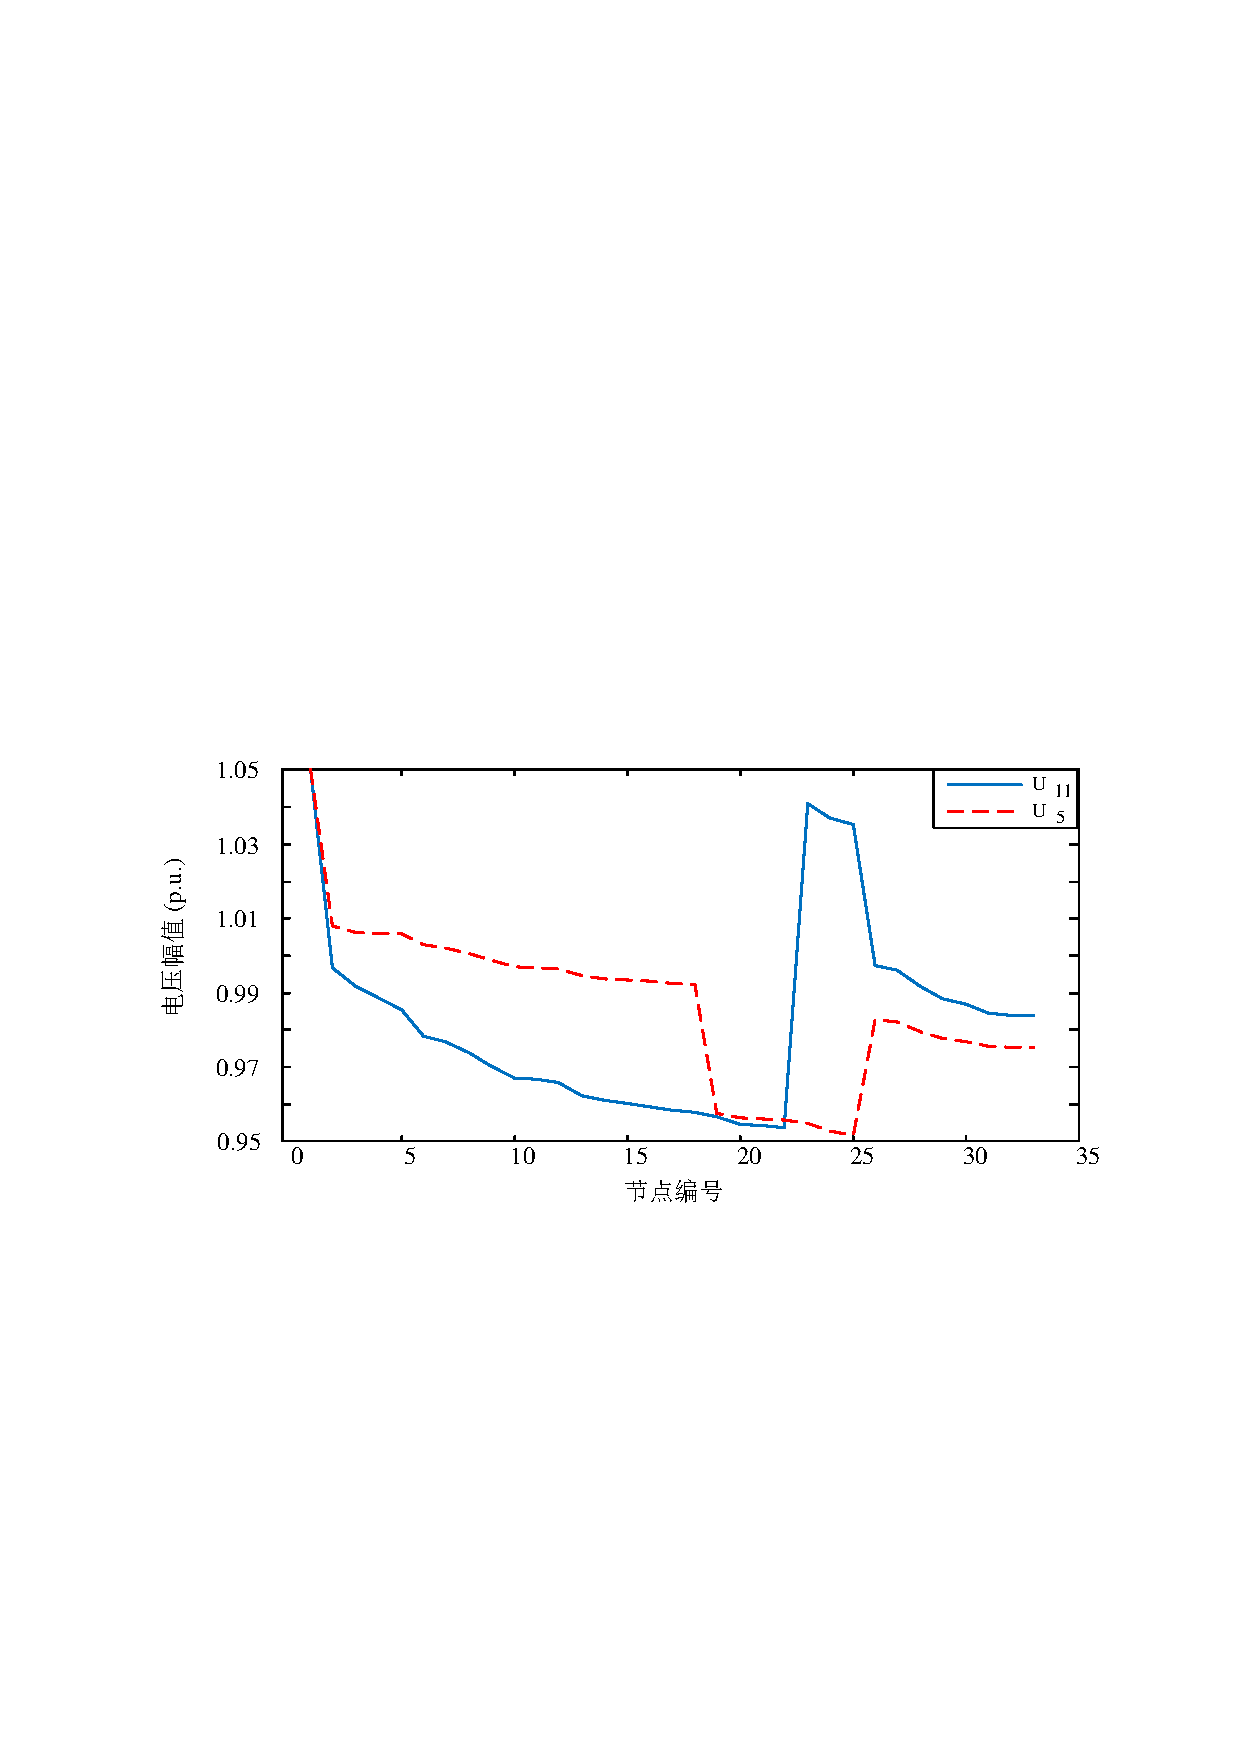
\includegraphics[scale=0.76]{figures/Chap4-15-Hub-Dispatch-Exe-Bus-Vol.pdf}
\caption{配电网节点电压分布}
\label{Fig:Hub-Dispatch-Exe-Bus-Vol}
\end{figure}

\begin{figure}[H]
\centering
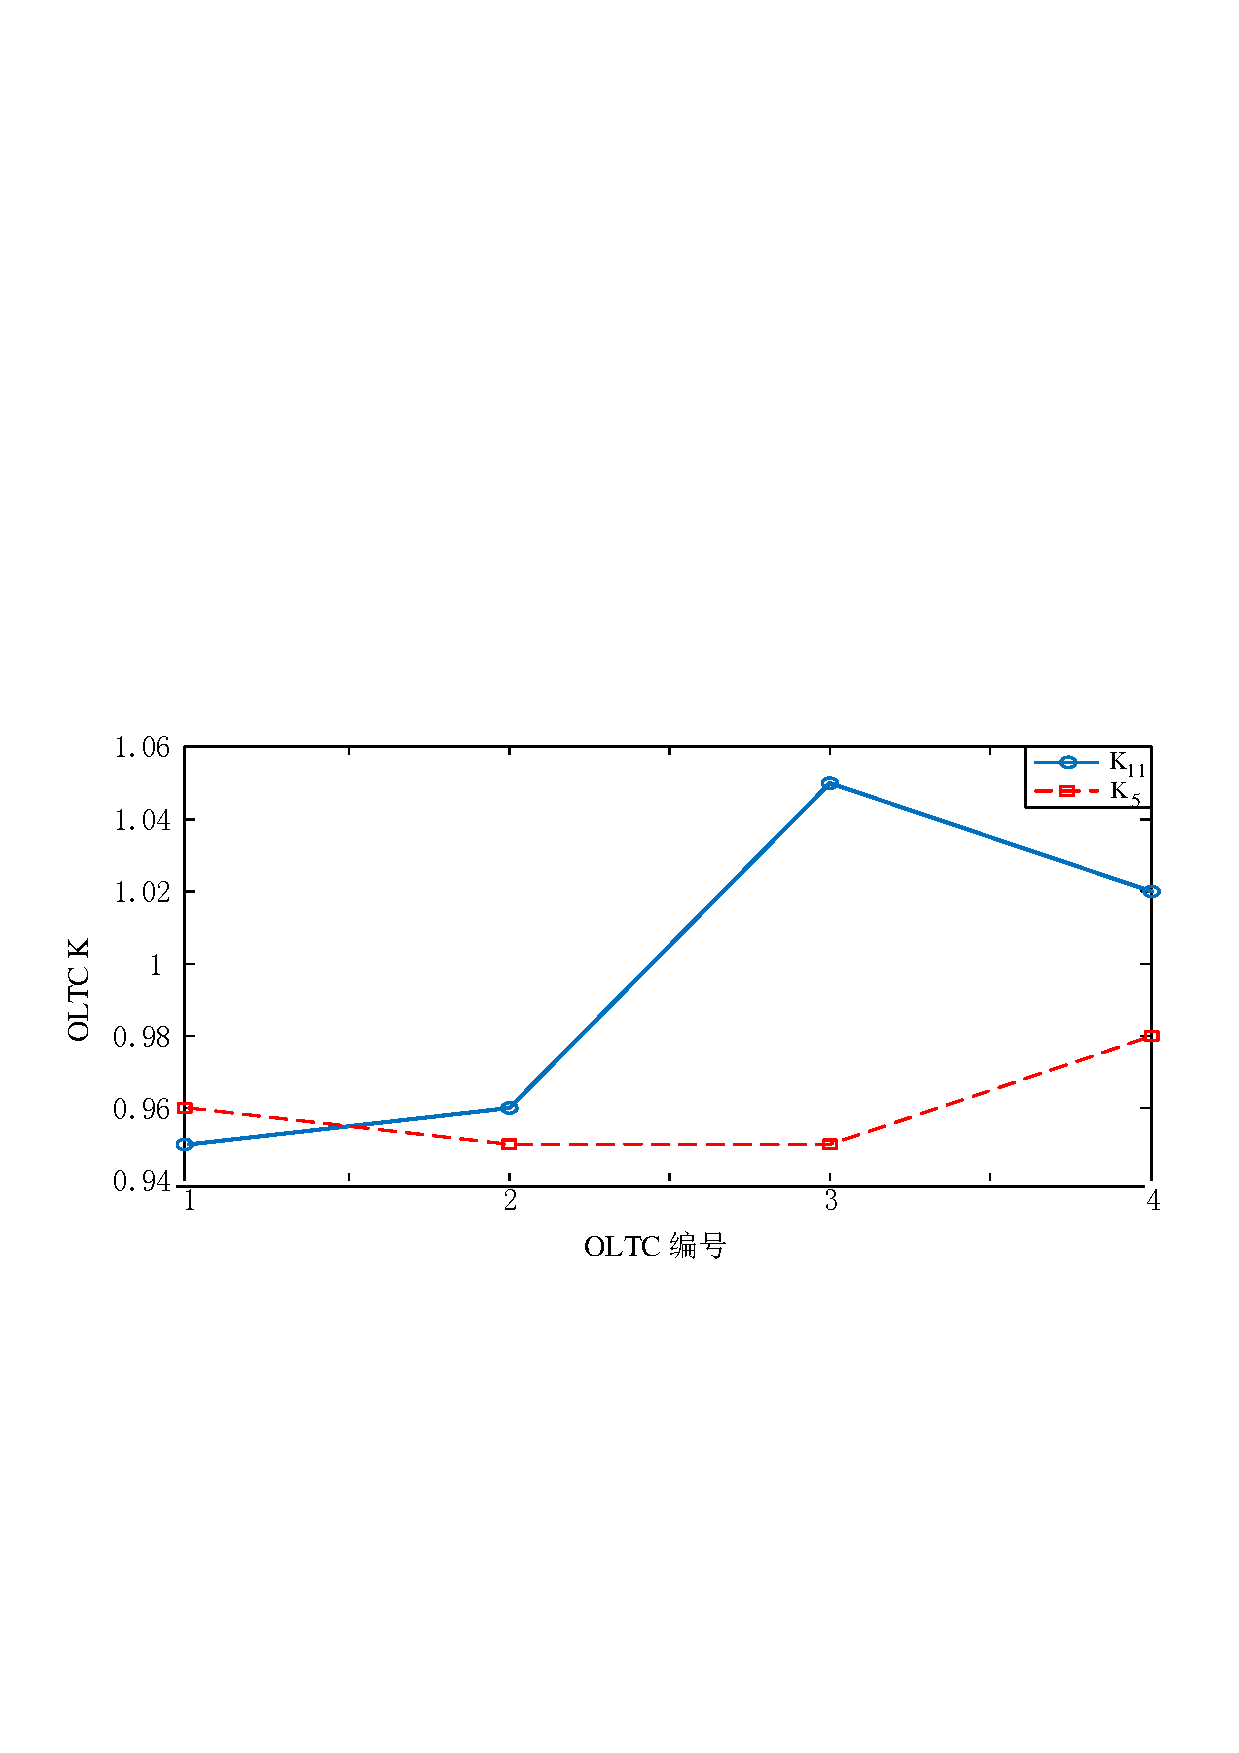
\includegraphics[scale=0.65]{figures/Chap4-15-Hub-Dispatch-Exe-OLTC-K.pdf}
\caption{OLTC分接头状态分布}
\label{Fig:Hub-Dispatch-Exe-OLTC-K}
\end{figure}

区域供热网络在热负荷峰值时段5以及非峰值时段15的最优温度分布如图~\ref{Fig:Hub-Dispatch-Exe-Pipe-Temp}所示。通过调节回水温度可以满足高峰期(时段15)和非高峰期(时段5)不同的热功率需求。在供水温度相同的情况下,回水温度越小,供热量越大。此外,由于供热管网的摩擦、传热损耗等,供水和回水系统中管道出口的水温通常低于入口温度。

\begin{figure}[H]
\centering
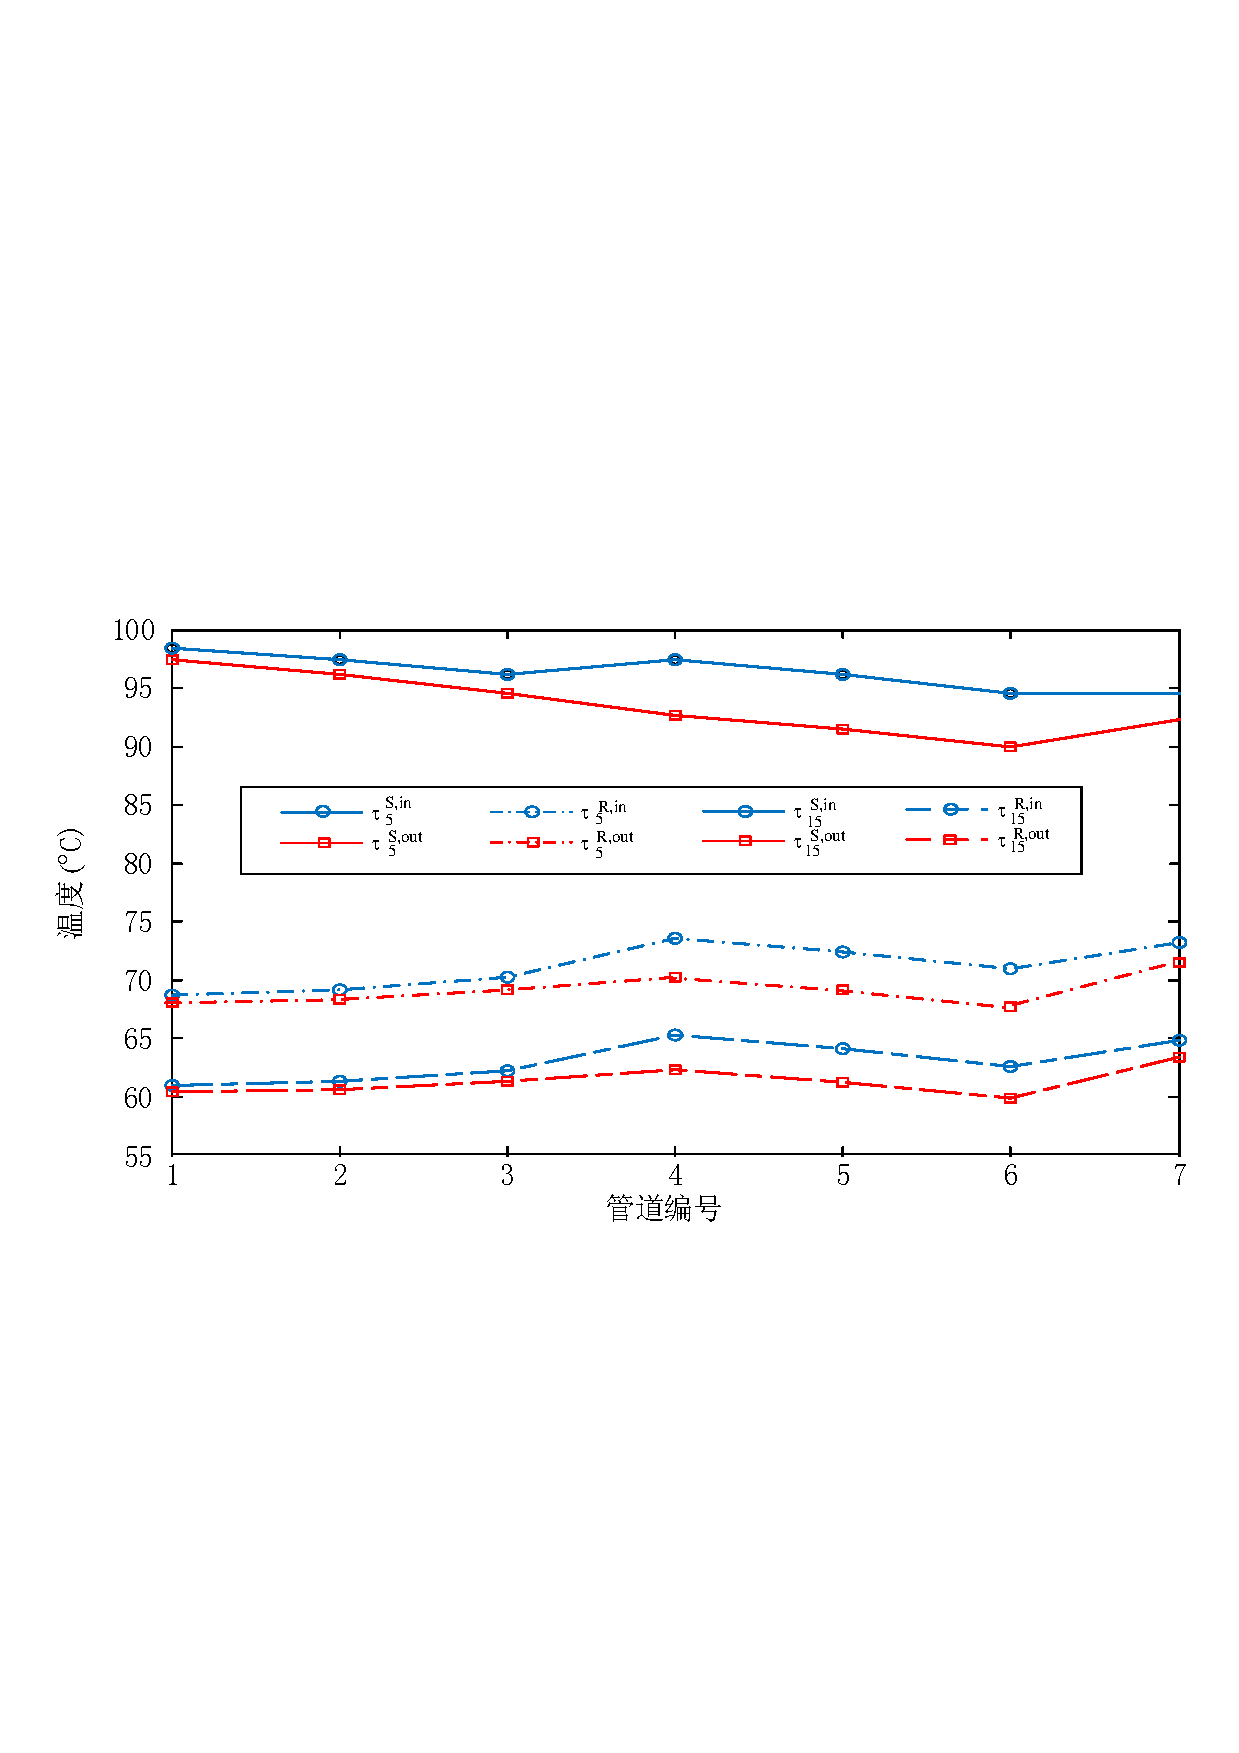
\includegraphics[scale=0.62]{figures/Chap4-15-Hub-Dispatch-Exe-Pipe-Temp.pdf}
\caption{供热网络温度分布}
\label{Fig:Hub-Dispatch-Exe-Pipe-Temp}
\end{figure}

%\begin{figure}[H]
%\centering
%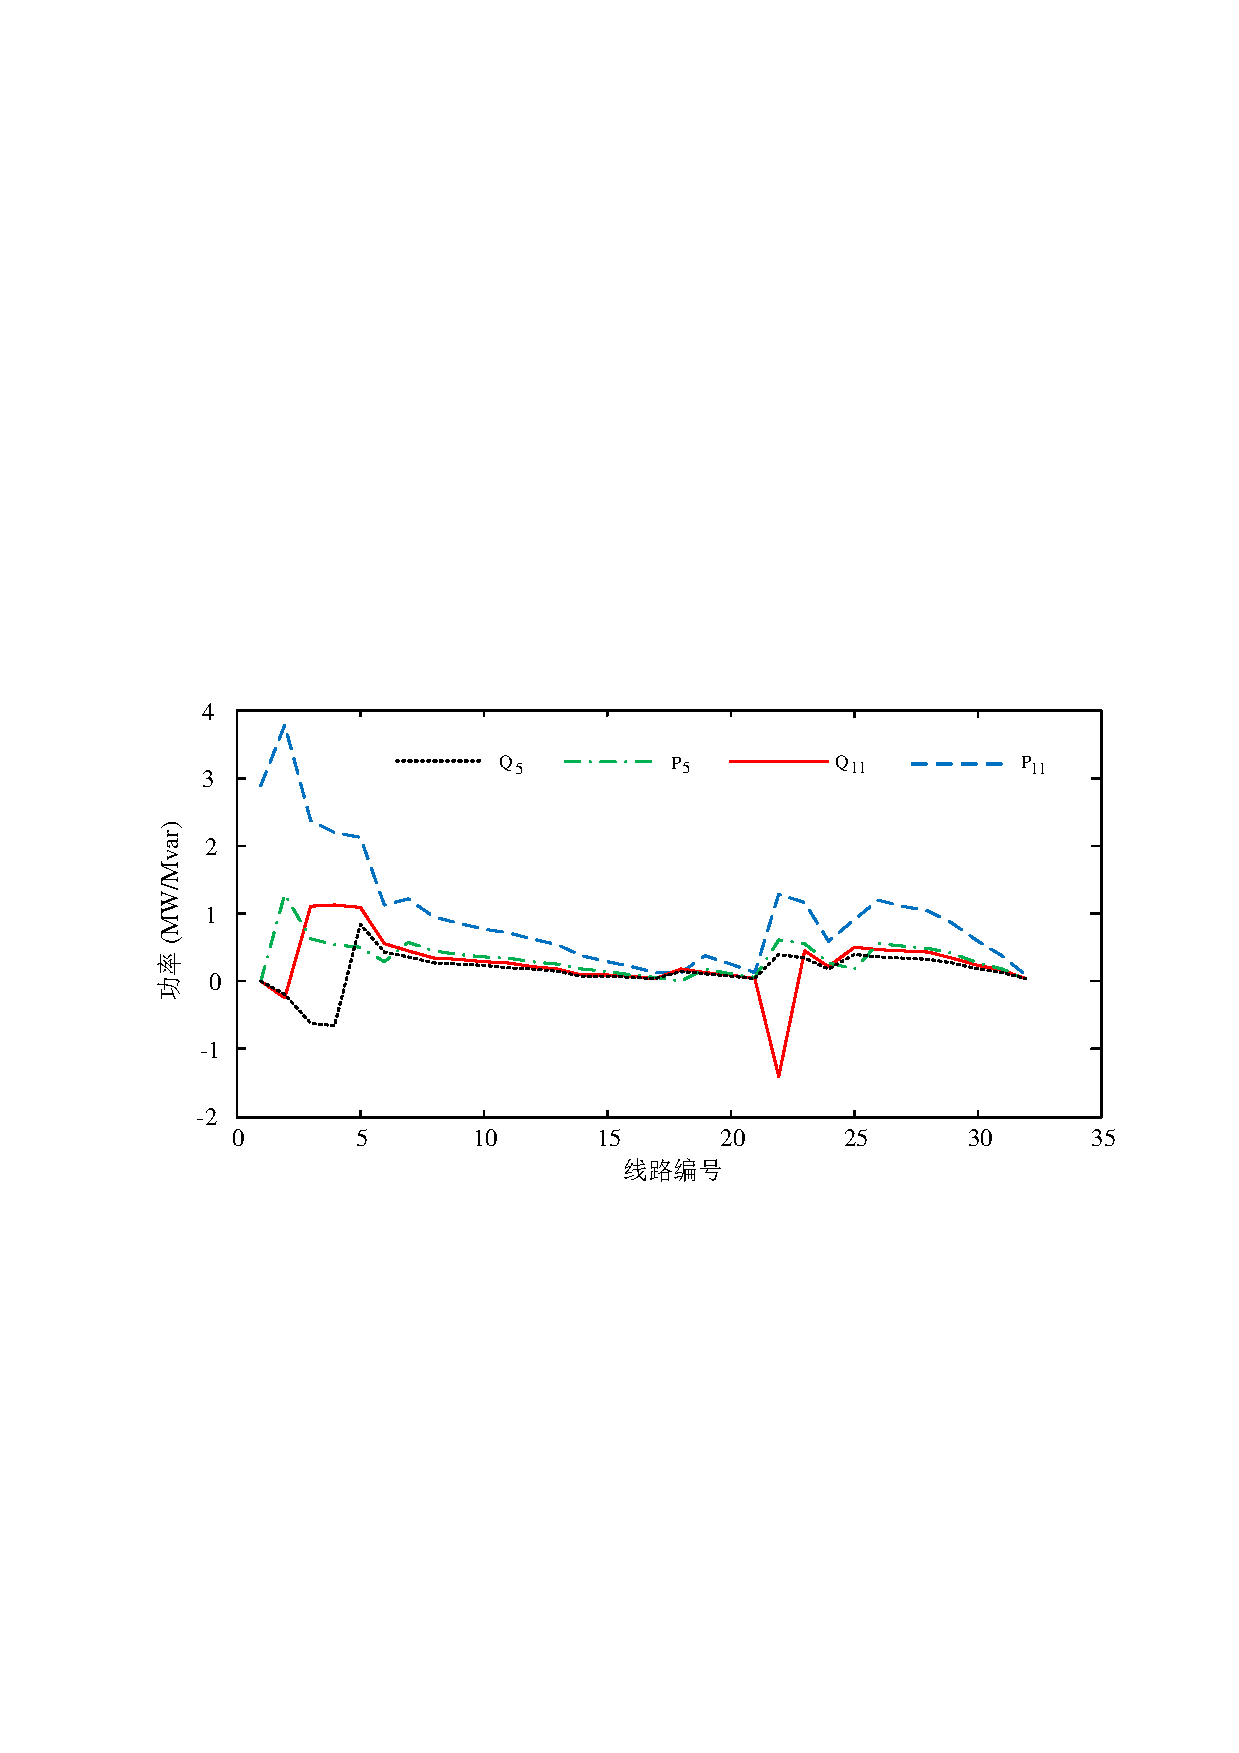
\includegraphics[scale=0.70]{figures/Chap4-15-Hub-Dispatch-Exe-Line-PQ.pdf}
%\caption{配电网线路潮流分布}
%\label{Fig:Hub-Dispatch-Exe-Line-PQ}
%\end{figure}


\section{基于㶲理论的热电质量-数量联合运行模型}
\label{sec:exergy-IES-model}
正如第~\ref{sec:st-caes-dispatch}节运行调度分析一致,热电综合能源系统旨在发挥热、电等多能流载体的协同效应,而多能流协同必须考虑能流间的统一性与差异性。现有研究主要基于多能流间的统一性,将电、热等能流载体单独研究的工具与方法(如潮流分析等)引入综合能源系统分析中,采用基于热力学第一定律的“能量平衡法”研究多能源系统中的能量流,如DHN潮流模型(\ref{eq:DHN-Thermal-Part})-(\ref{eq:DHN-heat-power-model})与PDN潮流模型(\ref{eq:PDN-Branch-Flow-All})。 然而,该类“能量平衡法”难以刻画多能流载体间的差异性,特别是能流品位的差异性。本节基于热力学第二定律的“㶲”(最大有效能)理论\cite{Eng-Thermo-83}研究热电综合能源系统的“数量- 质量”联合建模问题。我们采用“焓㶲”刻画管网中稳流工质的㶲流,并用“热量㶲”描述热源与热负荷的㶲输出及㶲需求,以实现“温度对口,梯级利用”的热能传输,为供热管网及含AA-CAES能量枢纽的热电综合能源系统的运行提供新的分析视角。

\subsection{热网质量-数量联合模型}
\label{sec:DHN-Exergy-Model}
假定针对图~\ref{Fig:DHN-Topology-Exergy}所示的区域供热网络已进行网潮流(\ref{eq:DHN-Thermal-Part})-(\ref{eq:DHN-heat-power-model})分析。为此,可进一步建立热源节点的㶲平衡方程为,
\begin{subequations}
\label{eq:exergy-heat-source}
\begin{gather}
\dot Ex_i^S = {{\dot m}_i^g}{(({h_i^S - {h_0}}) - {T_0}({s_i^S - {s_0}}))}\\
\dot Ex_i^R = {{\dot m}_i^g}{(({h_i^R - {h_0}}) - {T_0}({s_i^R - {s_0}}))} \\
\Delta \dot Ex_i^g = \frac{{2{T_0}}}{{\left( {\tau_i^S + \tau_i^R} \right)}}W_i^g\\
W_i^g + \dot Ex_i^g = \dot Ex_i^S - \dot Ex_i^R + \Delta \dot Ex_i^g
\end{gather}
\end{subequations}
其中,$\dot Ex_i^S$ 与 $\dot Ex_i^R$ 分别为流经热源节点的供水与回水焓㶲;$h$ 与 $s$ 分别为热水在相应状态点(由压力和温度描述)的焓与熵;下标 0表示环境状态或均衡态;$\Delta \dot Ex_i^g$ 表示通过消耗电能由热泵产生的㶲损失;$W_i^g$为热源中循环水泵消耗的电能。

\begin{figure}[H]
\centering
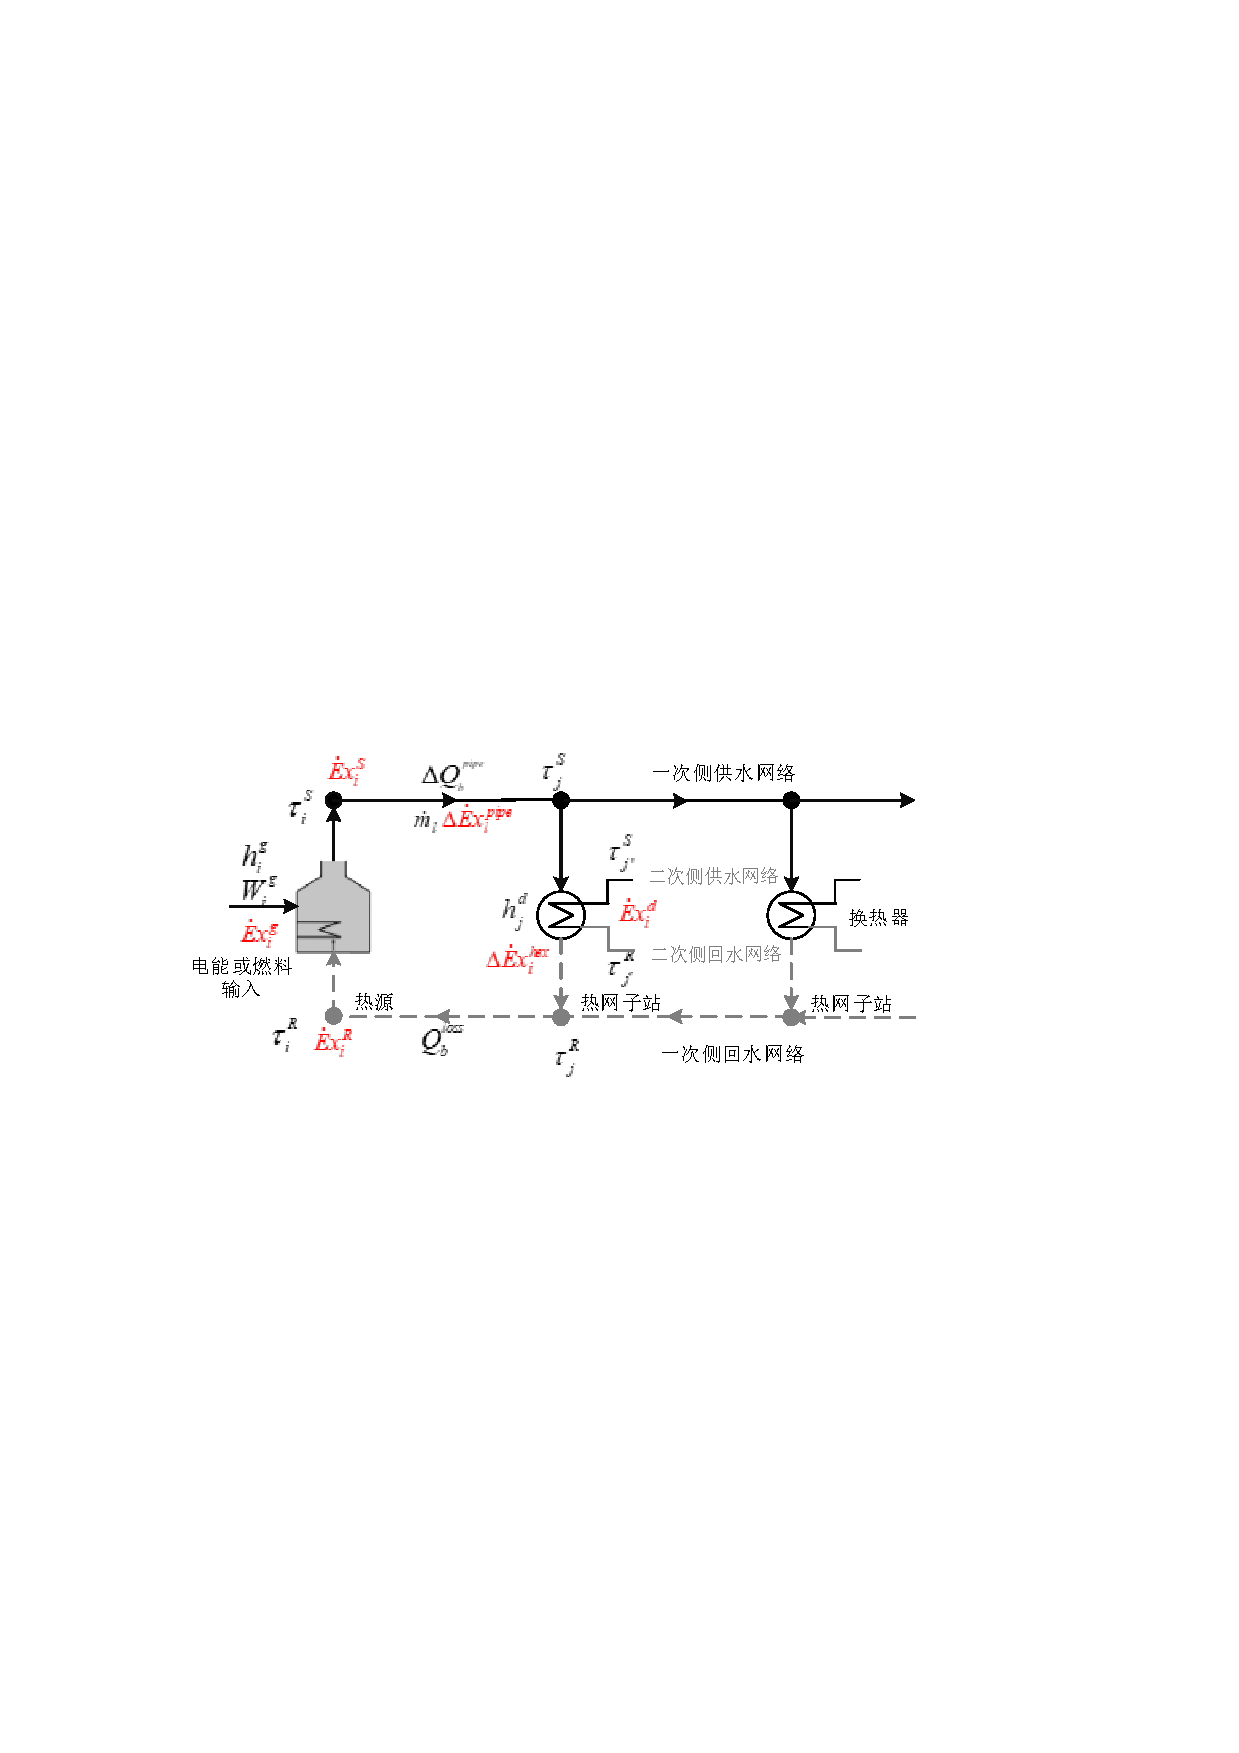
\includegraphics[scale=0.79]{figures/chap4-4-DHN-Exergy-Model-V2.pdf}
\caption{区域供热网络㶲流示意图}
\label{Fig:DHN-Topology-Exergy}
\end{figure}

供水及回水管网的㶲流损失可表示为,
\begin{subequations}
\label{eq:Exergy-loss-pipe}
\begin{gather}
\Delta \dot Ex_b^{pipe} = Ex_{b(i)}^S - Ex_{b(j)}^S + Ex_{b(j)}^R - Ex_{b(i)}^R \label{eq:Exergy-loss-pipe-V1}\\
\Delta \dot Ex_b^{pipe} = ({1 - \frac{{2{T_0}}}{{\tau_{b(i)}^S + \tau_{b(i)}^R}}})\Delta Q_b^{pipe} \label{eq:Exergy-loss-pipe-V2}
\end{gather}
\end{subequations}
其中,$\Delta \dot Ex_l^{pipe}$ 为管道$b$的㶲损;$\Delta \dot Q_b^{pipe}$为管道的热能损失,可由管道出口与入口温度计算而来。若尚未对DHN进行模型(\ref{eq:DHN-Thermal-Part})-(\ref{eq:DHN-heat-power-model}) 中的热力与水力状态分析,则可用(\ref{eq:Exergy-loss-pipe-V1}) 分析管道㶲损;若已对DHN进行了热力与水力状态分析,可采用(\ref{eq:Exergy-loss-pipe-V2}) 进行管道㶲损的分析。

热力负荷子站(或换热器)中的㶲流损失为,
\begin{subequations}
\label{eq:Exergy-loss-heat-exchanger}
\begin{gather}
\Delta \dot Ex_j^{hex} = {T_0}h_j^d({\frac{2}{{\tau_j^S + \tau_j^R}} - \frac{2}{{\tau_{j'}^S + \tau_{j'}^R}}})\\
\dot Ex_j^d = h_j^d({1 - \frac{{2{T_0}}}{{\tau_{j'}^S + \tau_{j'}^R}}})
\end{gather}
\end{subequations}
其中,$\Delta \dot Ex_j^{hex}$ 表示连接热网一次侧与二次侧的热力站内部的不可逆换热过程导致的㶲损,通常该部分㶲损占据了整个供热管网㶲损的主要部分;$\tau_{j'}^S$ 与 $\tau_{j'}^R$ 分别为供热管网二次侧采用的温度机制,通常连接于同于供热管网的不同热力子站,如工业热力子站、商业子站及民用子站采用不同的二次侧温度机制;$\dot Ex_j^d$表示热负荷获取的㶲能。

%针对仅电力系统应用场景,压缩空气储能对外的能量接口形式为电能。研究从热力学特性视角分析了压缩空气储能内部压缩机、透平等能量转换单元的功-能转换特性与宽工况特性,建立了包含储气库与高温储热罐两个能量储存单元的双State-of-Charge模型;通过换热器等能量转移单元的热力学特性实现了“双SOC模型”中储气水平SOC与储热水平SOC 间的耦合,系统地解决了宽工况与多能流耦合导致的压缩空气储能稳态运行建模难题。
%
%针对多能源系统应用场景,压缩空气储能对外的能量接口形式为冷、热、电,对内的能量转换载体为压力势能与压缩热能。本节研究从“㶲分析”视角出发,建立了集内部压力势能与压缩热能、外部冷-热- 电输出等不同品位能量的压缩空气储能“㶲平衡模型”,为辨识压缩空气能量枢纽内部重要㶲损组件以及提高压缩空气储能能量枢纽综合能效提供了新视角,同时也为广义能流中“㶲分析理论”提供了能量枢纽级的“㶲接口”。

\subsection{综合能源系统质量-数量联合模型}
\label{sec:exergy-IES-Interface}
基于热网㶲流模型(\ref{eq:exergy-heat-source})-(\ref{eq:Exergy-loss-heat-exchanger}) 可进一步建立热电综合能源系统质量-数量联合模型(即㶲模型),以实现对现有分析理论的兼容性,主要表现在基于“电能品位为1”的物理事实,电网的传统能量平衡模型(如(\ref{eq:PDN-Branch-Flow-All}))即为㶲模型,即与热网的质量-数量联合模型直接兼容。同时,任何热电能量枢纽的模型只需对外提供“㶲接口”便可兼容质量-数量联合模型,从而将热电综合能源系统㶲模型的核心转移到自带多能流特性的能量枢纽,如本章重点关注的热电联供型AA-CAES。为此,可基于第2章中的AA-CAES㶲仿真模型(\ref{eq:exergy-compressor})-(\ref{eq:exergy-TV})作为㶲接口,整体实现含AA-CAES型能量枢纽的区域热电综合能源系统的质量与能量联合建模。

\subsection{单热源双负荷系统算例分析}
本小节仅针对热网进行质量-数量联合建模分析,以说明㶲分析模型的必要性。针对含AA-CAES型能量枢纽的热电综合能源系统,可按第\ref{sec:exergy-IES-Interface}节中的思路展开分析,此处不予探讨。考虑图~\ref{Fig:DHN-Exergy-Case}所示单热源双负荷系统,假设热源部署于节点1,节点2 为具有高品位热能需求的商业热力子站,节点3 为具有较低品位热能需求的民用热力子站,但节点2 与节点3 的热负荷功率需求相同。管网一次侧采用95$^{\circ}$C/40$^{\circ}$C的供回水温度机制,并设定环境温度为15$^{\circ}$C。商业子站二次侧采用75$^{\circ}$C/30$^{\circ}$C 的供回水温度机制,而民用热力子站二次侧采用55$^{\circ}$C/30$^{\circ}$C的供回水温度机制。此外,做如下假设:1)假定忽略沿管道的压力损失,供回水管道之间的压差为16~bar,泵效率为0.8;2)假定环境温度为15$^{\circ}$C;3)管道温度损失系数为 0.15$\times ^{-3}$ kW/(m$\cdot$K),两条管道长度均为1000m;4)负荷通过换热器从供热管网取热,假设忽略换热器传热的㶲损失。

\begin{figure}[!htp]
\centering
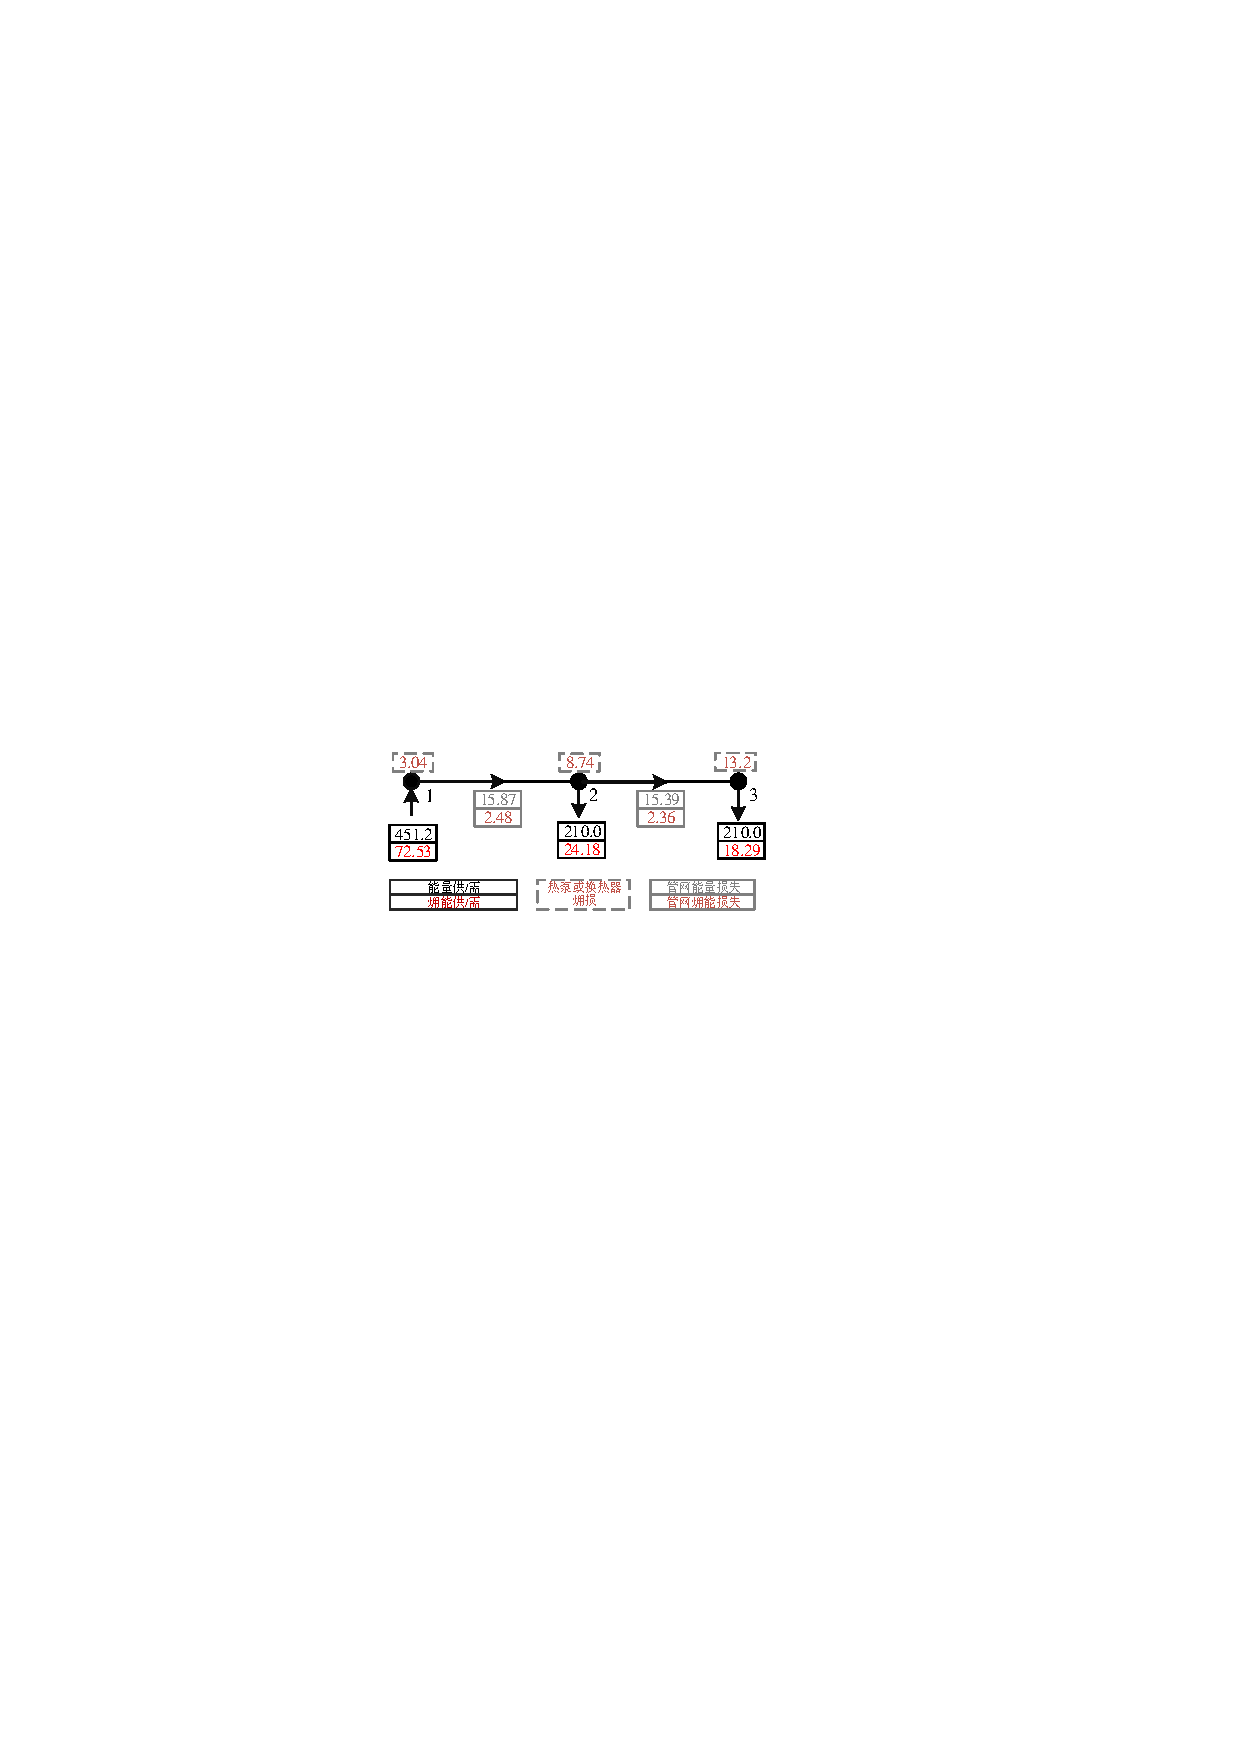
\includegraphics[scale=1.35]{figures/Chap4-6-DHN-Exergy-Case.pdf}
\caption{单热源双负荷系统㶲分析结果}
\label{Fig:DHN-Exergy-Case}
\end{figure}

采用㶲分析模型(\ref{eq:exergy-heat-source})-(\ref{eq:Exergy-loss-heat-exchanger}) 的㶲分析结果示于图~\ref{Fig:DHN-Exergy-Case}~中,图中的热功率与㶲的单位均为kW。尽管商业热力子站与民用热力子站的热功率需求均为 210 kW,但是二者从一次管网中获取了不同的热能产品。前者获取了75$^\circ$C/30$^\circ$C的热水,而后者获取了55$^\circ$C/30$^\circ$C的热水,其㶲分别为24.18 kW 与 18.28 kW,即商业热力子站获取了高品位的热能,而民用热能子站获取了较低品位的热能。系统总的热功率损失为6.93$\%$, 而㶲损达39.38$\%$。因此,在区域热电综合能源系统优化和运行中考虑能量品位很有必要。

综上,基于热力学第一定律的经典热力-水力工质流模型不能考虑能量品位,而本节所提的㶲分析模型基于热力学第二定律,可以同时考虑热能数量与热能品位。此外,㶲分析模型提供的能量数量及品位的损失信息可以为区域热电综合系统中的多能流产品定价等问题提供参考。

\section{面向热电综合能源市场的能量枢纽竞标策略}
\label{sec:bid-st-caes}
气、热、电等多能源网络互联构建综合能源系统被认为是增强能源网络灵活性与可靠性的一种有效手段,而综合能源系统中实现气、电、热等网络互联的关键设备即为能量枢纽。随着配电市场的完善\cite{PDN-Market-2}及热力市场的逐渐成熟\cite{Heat-Market-C2,Heat-Market-C4},该类能量枢纽将有望作为独立市场运营主体\cite{EH-Bid-18} 参与区域配电网和区域热网中热电两个能流的交易\cite{EH-Bid-Rui-18},其在多能流交易市场的策略竞价是提升运营经济性的关键。目前针对电源、负荷及储能设备在电力市场的竞价策略已有大量研究成果\cite{PDN-Market-1,Thesis-Shafiee},但均针对电力单一能流交易,难以直接推广到AA-CAES型或其它能量枢纽在多能流市场中的运营。综合能源系统工程实际迫切需要开展面向多能流市场交易的能量枢纽的竞价策略研究,本节将给出一种适用于以第三方主体独立运营的能量枢纽(如II型AA-CAES热电能量枢纽)的多能流市场竞标策略。

\subsection{AA-CAES型能量枢纽竞标模型}
\subsubsection{假设条件}
本节以图~\ref{fig:AA-CAES-Hub-V2}所示的II型AA-CAES能量枢纽为例,重点分析供能灵活性(热电联供与热电联储)赋予其在热力市场、电力市场(及燃料市场)的竞标行为,以提升该类能量枢纽的运行经济性。本节做如下假设:

1)聚焦于日前电力与热力市场,采用负荷预测并忽略不确定性\footnote{第\ref{sec:bid-eh-con-uncert}节将给出计及不确定性的扩展方法。},不考虑用于平衡供需不匹配的实时市场。不同于第\ref{sec:st-caes-dispatch}节中采用的热电综合能源系统的集中运营假设,本节假定电力市场与热力市场分别由独立的运营商管理,即电力市场操作员(EMO)和热力市场操作员(HMO)。

2)供热网络与供电网络通过II型AA-CAES能量枢纽实现耦合,电网潮流采用线性化的DistFlow潮流模型(\ref{eq:Lin-Dist-Flow-Non-OLTC});供热网络采用固定质量流率(即CF-VT调节模式)的水力-热力耦合模型(\ref{eq:DHN-Thermal-Part})-(\ref{eq:DHN-heat-power-model})。II型能量枢纽分别向热网与电网上报竞标价格与数量,~EMO~与~HMO~ 以最小化生产成本分别出清电力与热力市场。

3)能量枢纽面向电力与热力市场的竞标策略间通过其内部的能量转换与存储单元实现了耦合。EMO与HMO以报价结算方式\cite{Pay-as-Bid-08,Pay-as-Bid-RL-agent-17} 清算能量枢纽的收益,该结算方式在配电市场中得到普遍应用。此外,能量枢纽上报的竞标价格通过与EMO和HMO的协议进行相应限制。

\subsubsection{热力市场出清问题}

由第~\ref{sec:st-caes-dispatch}~节的区域供热管网潮流模型(\ref{eq:DHN-Thermal-Part})-(\ref{eq:DHN-heat-power-model})可知,DHN的运行状态可由供回水管网的入口与出口温度,以及实现供回水管道耦合的热源与热负荷的供回水温度给定。若将所有的温度变量统一记为向量~$\rm \tau$~,用向量~$\bf h$~表征热源输出功率,并用向量$\dot {\bf m}$表示所有管道的质量流率,则~DHN~潮流(\ref{eq:DHN-Thermal-Part})-(\ref{eq:DHN-heat-power-model})的紧凑形式可表示为,
\begin{subequations}
\label{eq:DHN-TF-Comp}
\begin{align}
A_H{\bf h} + B_H(\dot {\bf m})\tau = b_H\label{eq:DHN-TF-Comp-EQ}\\
C_H{\bf h} + D_H(\dot {\bf m})\tau \le d_H \label{eq:DHN-TF-Comp-IN}
\end{align}
\end{subequations}
其中,~$A_H$, ~$b_H$, ~$C_H$ 和 ~$d_H$ 分别为常系数矩阵;~$B_H(\dot {\bf m})$~ 及~$D_H(\dot {\bf m})$~ 表示依赖于~$\dot {\bf m}$的系数矩阵;热网潮流(\ref{eq:DHN-Thermal-Part})-(\ref{eq:DHN-heat-power-model})体现于 (\ref{eq:DHN-TF-Comp-EQ}) 中;$\tau$与 $\bf h$ 的上下界体现于(\ref{eq:DHN-TF-Comp-IN}) 中。显然,紧凑型DHN模型(\ref{eq:DHN-TF-Comp})为非线性且非凸。本节假定~DHN~运行于固定质量流率模式,即$\dot {\bf m}$ 为定值,如此约束集(\ref{eq:DHN-TF-Comp})退化为以节点温度~$\rm \tau$~和热源输出功率${\bf h}$为决策变量的线性模型。

供热市场操作员HMO以实现AA-CAES型能量枢纽、燃气锅炉等热源间的经济调度为决策目标。从能量平衡的角度来看,热网运行成本在很大程度上依赖于热源的输出功率,其值等于热负荷与管道损失之和。事实上,$\dot {\bf m}$ 对管道热损失的影响较小。管道热损失可简化表示为,
\begin{equation}
\label{eq:Pipe-Loss-Q}
\Delta E = c_p \dot m (\tau^{in}-\tau^{out})
\end{equation}
将管道出口温度方程~(\ref{eq:DHN-Pipe-Loss-S})或~(\ref{eq:DHN-Pipe-Loss-R})代入~(\ref{eq:Pipe-Loss-Q})~可得\footnote{为了表示简洁,此处我们去掉了$\dot m$ 的下标。},
\begin{equation}
\label{eq:Delta-E-App}
\Delta E = c_p \dot m [ (\tau^{in}- \tau^{am})(1-{\rm e}^{-\frac{\lambda_b l_b}{c_p \dot m}})]
\end{equation}
其中,$0 < \lambda_b l_b/c_p \dot m \ll 1$。考虑到,${\rm e}^{-x} \approx 1-x$,则(\ref{eq:Delta-E-App})可近似为,
\begin{equation}
\Delta E \approx c_p \dot m (\tau^{in}-\tau^{am}) \frac{\lambda_b l_b}{c_p \dot m} = \lambda_b l_b(\tau^{in} - \tau^{am})
\end{equation}
由此可知,$\Delta E$不依赖于$\dot m$。换言之,只要约束集(\ref{eq:DHN-TF-Comp})可行,供热管网水力条件对网络整体运行成本的影响不大。因此, $\dot {\bf m}$可被提前设置,即固定质量流率-变供水温度的运行模式~\cite{DHN-CFVT-2013}。

尽管电热泵、能量枢纽(如AA-CAES型)等电制热供暖方式逐渐成为新一代热网中的热源\cite{4th-DHN-14},但传统燃煤及燃气锅炉等仍为当前供热网络中的主要热力机组。因此,我们假定本节研究的~DHN~中含有燃煤及燃气锅炉等传统热源,其生产成本是其输出的凸二次函数。AA-CAES型能量枢纽向热力市场上报的竞标标的(热价~$\zeta^b$~与最大供热功率~$h_m^b$~),在热力市场出清问题中被视为常数。从而,热力市场出清模型为,
\begin{subequations}
\label{eq:HM-Clearing}
\begin{align}
\min_{{\bf h}, \tau}~~ & \frac{1}{2} {\bf h}^T Q_H {\bf h} + {\bf c}^T_h (\zeta^b) {\bf h}
\label{eq:HM-Clearing-Obj}  \\
\mbox{s.t.} ~~ &A_H{\bf h} + B_H(\dot {\bf m})\tau = b_H \label{eq:HM-Clearing-Cons-EQ}\\
       & C_H{\bf h} + D_H(\dot {\bf m})\tau \le d_H(h^b_m)
\label{eq:HM-Clearing-Cons-IN}
\end{align}
\end{subequations}
其中,目标函数(\ref{eq:HM-Clearing-Obj})最小化运行成本,包括传统锅炉的成本及给AA-CAES型能量枢纽的支出;(\ref{eq:HM-Clearing-Cons-EQ}) 与 (\ref{eq:HM-Clearing-Cons-IN}) 为紧凑型热网潮流模型。由于问题(\ref{eq:HM-Clearing}) 是凸二次规划问题,其~KKT~系统是充要条件。

\subsubsection{电力市场出清问题}
AA-CAES型能量枢纽向电力市场上报的竞标标的为售电电价~$\xi^b$~ 与购电电价~$\chi^b$~,类似于热力市场出清,假定电力调度员以最小化调度成本为出清目标,即
\begin{equation}
C_{PDN} =  \sum_j \left[ a_j (p_j^g)^2 + b_j p_j^g \right]
+ \xi^b p^{gb}  - \chi^b p^{db}
\end{equation}
其中,第一项表示发电成本,$(a_j,b_j)$为二次成本系数;定义~$p^g_0 = \sum_{j \in \pi(0)} P_{0j}$~为从上级输电网(电力批发市场)输送到~PDN~的馈入电功率,$a_0=0$,$b_0$ 为上级电力市场电价;第二项(三项)是支付(收入)能量枢纽的购电(售电)$p^{gb}$ ($p^{db}$)的成本(收益)。

定义向量~$\bf p$~为发电调度~$p^g_j$~与能量枢纽的能量交易~$p^{gb}$~, ~$p^{db}$~;~$p_m^{gb}$~与~$p_m^{db}$~分别为能量枢纽愿意售出及购买的最大功率,~$\bf x$~ 为其它变量。如此,基于~\ref{sec:st-case-dispatch-PDN}节线性化DistFlow电网潮流模型,电力市场出清的紧凑型模型可表示为,
\begin{subequations}
\label{eq:PM-Clearing}
\begin{align}
\min_{\bf p,x}~~ & \frac{1}{2} {\bf p}^T Q_P {\bf p} + {\bf c}^T_p (\xi^b,\chi^b) {\bf p}   \label{eq:PM-Clearing-Obj}  \\
\mbox{s.t.} ~~ &  A_P {\bf p} + B_P {\bf x} = {\bf b}_P
\label{eq:PM-Clearing-Cons-EQ}  \\
       & C_P {\bf p} + D_P {\bf x} \le {\bf d}_P(p^{gb}_m, p^{db}_m)
\label{eq:PM-Clearing-Cons-IN}
\end{align}
\end{subequations}
其中,(\ref{eq:PM-Clearing-Cons-EQ})代表等式约束(\ref{eq:PF-P})-(\ref{eq:PF-U});(\ref{eq:PM-Clearing-Cons-IN})代表决策变量的上下界。与热力市场出清问题(\ref{eq:HM-Clearing})类似,电力市场出清问题亦为凸二次规划,其KKT系统是充要条件。

\subsubsection{能量枢纽竞标模型}
在市场运营问题中,AA-CAES型能量枢纽实际的功率输入与功率输出($p_t^{gas}$, $p_t^{gb}$ , $p_t^{db}$ 及$h_t^b$ )不能由其直接控制,而是由市场竞标结果决定,其竞标标的($p_{t,m}^{gb}$, $p_{t,m}^{db}$, $h_{t,m}^{b}$ )的上下界分别由下式给定,
\begin{subequations}
\label{eq:EH-Bid-Cons}
\begin{gather}
p_{\min }^{gb} \le p_{t,m}^{gb} \le p_{\max }^{gb}, ~\forall t \label{eq:EH-E-offer} \\
p_{\min }^{db} \le p_{t,m}^{db} \le p_{\max }^{db}, ~\forall t \label{eq:EH-E-bid} \\
h_{\min }^b \le h_{t,m}^b \le h_{\max }^b, ~\forall t \label{eq:EH-H-offer}
\end{gather}
\end{subequations}
其中,$p_{t,m}^{gb}$ 与 $p_{t,m}^{db}$ 分别表示II型AA-CAES能量枢纽管理者向电力市场提交的电量供/需竞标标的;$h_{t,m}^b$为向热力市场提交的热功率竞标标的。

\begin{figure}
\centering
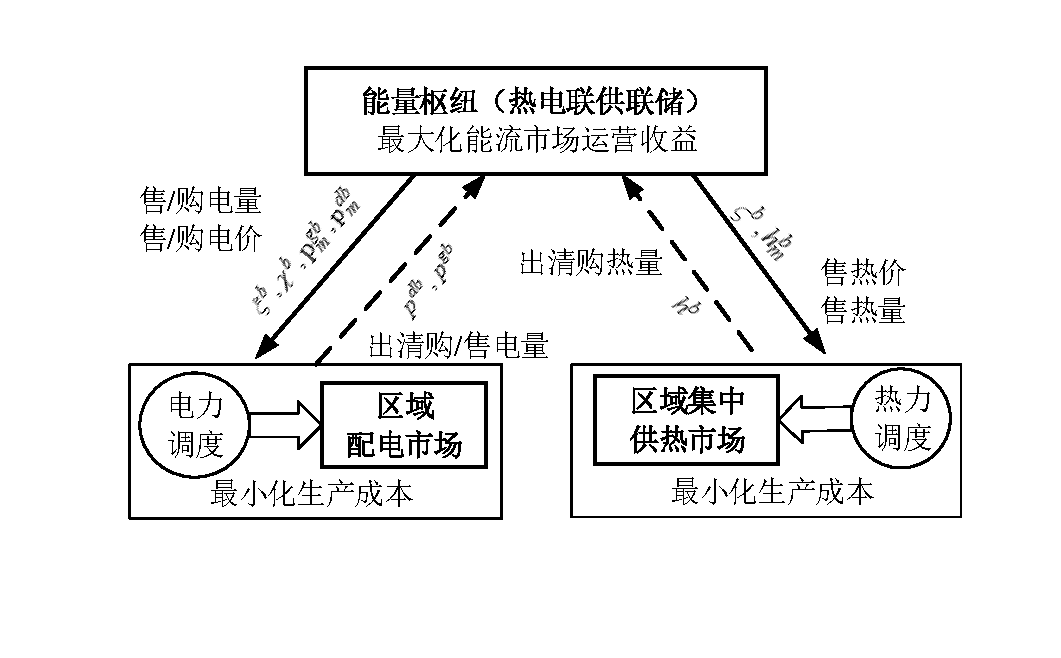
\includegraphics[scale=0.75]{figures/Chap4-5-EH-PAB-Struct.pdf}
\caption{AA-CAES能量枢纽热电市场竞标框架}
\label{Fig:Market}
\end{figure}

AA-CAES型能量枢纽竞标框架如图~\ref{Fig:Market}~所示,其日前电力与热力市场主从博弈竞标模型为,
\begin{subequations}
\label{eq:EH-Bidding}
\begin{align}
\max~ & (\bf \zeta^b)^T \bf h^b + (\bf \xi^b)^T {\bf p^{gb}} - {(\bf \chi^b)}^T {\bf p^{db}} - {(\bf \gamma)^T{\bf p^{gas}}} \label{eq:EH-Bid-Obj} \\
\mbox{s.t.}~ %& \mbox{Bounds of bidding strategies} \label{eq:EH-Quantity-bnd}\\
& \mbox{能量枢纽运行约束}~(\ref{eq:EH-Cons-II}) \label{eq:EH-Cons-2}\\
& \mbox{热力市场出清问题}~(\ref{eq:HM-Clearing}) \label{eq:EH-Bid-HM}\\
& \mbox{电力市场出清问题}~(\ref{eq:PM-Clearing}) \label{eq:EH-Bid-PM}\\
& \mbox{竞标标的约束集}~(\ref{eq:EH-Bid-Cons})
\end{align}
\end{subequations}
其中,价格向量~$\bf \zeta^b$,~$\bf \xi^b$,~$\chi^b$,~$\bf \gamma$~分别表示日前电力市场的热功率报价、电功率报价、储能电价及燃料价格; 能量交易向量~$\bf h^{b}$~, ~$\bf p^{gb}$,$\bf p^{db}$, $\bf p^{gas}$~分别表示出清热量,出清电量、购电量及燃气需求。(\ref{eq:EH-Cons-2})表示能量枢纽的运行约束;能量交易由电力市场出清(\ref{eq:EH-Bid-PM})与热力市场出清问题(\ref{eq:EH-Bid-HM})确定。由此,能量枢纽日前竞标模型为均衡约束的数学规划问题(MPEC)\cite{MPEC-Conejo-book-12}。从博弈视角看,MPEC 问题(\ref{eq:EH-Bid-PM}) 可视为Stackelberg博弈\cite{Game-Mei-16, Game-MIT-94},能量枢纽的最优策略和两个市场的出清结果即为该博弈的均衡。事实上,针对任一形式的热电能量枢纽,只要重新建模其运行约束(\ref{eq:EH-Cons-II}),竞标模型(\ref{eq:EH-Bidding})即可直接应用。

\subsection{模型求解策略}
本小节主要研究AA-CAES型能量枢纽双层竞标模型(\ref{eq:EH-Bidding})的高效求解策略。考虑到,市场出清问题(\ref{eq:HM-Clearing}) 与 (\ref{eq:PM-Clearing})均为凸二次规划,分别可由相应的KKT 最优性条件代替,从而可将双层模型(\ref{eq:EH-Bidding})转化为单层规划问题。

\subsubsection{单层竞标模型}

热力市场问题出清问题(\ref{eq:HM-Clearing})的最优性条件为,
\begin{subequations}
\label{eq:KKT-Heat}
\begin{align}
A_H{\bf h} + B_H(\dot {\bf m})\tau = b_H \label{eq:KKT-Heat-Eq0} \\
C_H{\bf h} + D_H(\dot {\bf m})\tau \le d_H(h^b_m) \label{eq:KKT-Heat-Eq1} \\
Q_H{\bf h} + {\bf c}_h (\zeta^b) + A_H^T \lambda_h + C_H^T \mu_h = {\bf 0} \label{eq:KKT-Heat-Eq2} \\
B_H(\dot {\bf m})\lambda_h + D_H^T(\dot {\bf m})\mu_h = 0,~
\mu_h \ge {\bf 0} \label{eq:KKT-Heat-Eq3} \\
{\mu_h ^T}( C_H {\bf h} + D_H (\dot {\bf m})\tau - d_H(h^b_m) )=0 \label{eq:KKT-Heat-Eq4}
\end{align}
\end{subequations}
其中,$\lambda_h$ 与 $\mu_h$ 分别为(\ref{eq:HM-Clearing}) 中等式约束和不等式约束的对偶变量;向量$d_H$ 与 ${\bf c}_h$ 是能量枢纽上报于热力市场的竞标标的 ($h^b_m$ 与 $\zeta^b$)的线性函数,二者在热力市场出清问题中被视为常数。 (\ref{eq:KKT-Heat-Eq0}) 与 (\ref{eq:KKT-Heat-Eq1})分别为热力市场出清问题原变量的可行性约束;(\ref{eq:KKT-Heat-Eq2}) 与 (\ref{eq:KKT-Heat-Eq3})分别为对偶变量的可行性约束;(\ref{eq:KKT-Heat-Eq4}) 为互补松弛条件。

相应地,电力市场出清问题(\ref{eq:PM-Clearing})的最优性条件为,
\begin{subequations}
\label{eq:KKT-Power}
\begin{align}
A_P {\bf p} + B_P {\bf x} = {\bf b}_P \label{eq:KKT-Power-Eq0}\\
C_P {\bf p} + D_P {\bf x} \le {\bf d}_P(p^{gb}_m, p^{db}_m) \label{eq:KKT-Power-Eq1}\\
Q_P {\bf p} + {\bf c}_p (\xi^b,\chi^b) + A_P^T \lambda_p + C_P^T \mu_p ={\bf 0} \label{eq:KKT-Power-Eq2}\\
B_P^T\lambda_p + D_P^T\mu_p = {\bf 0},~\mu_p \ge {\bf 0}  \label{eq:KKT-Power-Eq3}\\
\mu_p ^T ( C_P {\bf p} + D_P{\bf x} - {\bf d}_P(p^{gb}_m, p^{db}_m) ) = 0 \label{eq:KKT-Power-Eq4}
\end{align}
\end{subequations}
其中,$\lambda_p$ 与 $\mu_p$ 分别为(\ref{eq:PM-Clearing}) 中等式约束与不等式约束的对偶变量;向量${\bf c}_p$ 与 ${\bf d}_p$是能量枢纽上报于电力市场竞标标的 ($\xi^b$, $\chi^b$, $p^{gb}_m$ 与 $p^{db}_m$)的线性函数,这些竞标标的在电力市场出清问题中被视为常数。(\ref{eq:KKT-Power-Eq0}) 与 (\ref{eq:KKT-Power-Eq1}) 为电力市场出清问题原变量的可行性约束;(\ref{eq:KKT-Power-Eq2}) 与 (\ref{eq:KKT-Power-Eq3}) 分别为对偶变量的可行性约束;(\ref{eq:KKT-Power-Eq4})为互补松弛条件。

采用热力市场出清问题的KKT系统(\ref{eq:KKT-Heat})及电力市场出清问题的KKT系统(\ref{eq:KKT-Power})分别代替双层竞标模型(\ref{eq:EH-Bidding})中的(\ref{eq:EH-Bid-HM})及(\ref{eq:EH-Bid-PM})后,AA-CAES能量枢纽竞标模型(\ref{eq:EH-Bidding})将转化为易于进一步处理的单层优化问题。事实上,该单层优化问题仍为非线性模型,需进一步转化与处理。

\subsubsection{~MILP~近似模型}
由于互补松弛条件(\ref{eq:KKT-Heat-Eq4})与(\ref{eq:KKT-Power-Eq4})的存在,~KKT~系统(\ref{eq:KKT-Heat})与(\ref{eq:KKT-Power})仍为非线性非凸。同时,目标函数(\ref{eq:EH-Bid-Obj})中的~${(\bf \zeta^b)}^T {\bf h^{b}}$, ~${(\bf \xi^b)}^T {\bf p^{gb}}$,  ${(\bf \chi^b)}^T {\bf p^{db}}$等双线性项,也增加了单层竞标模型的求解难度。

针对互补松弛条件$\bf 0 \le  x \bot y \ge 0$,采用大~M~法\cite{Big-M-1981}线性化,
\begin{equation}
{\bf 0} \le {\bf x} \le M {\bf z},~
{\bf 0} \le {\bf y} \le M ({\bf 1-z})
\label{eq:bigM}
\end{equation}
其中,$\bf z$ 为与$\bf x$ 及$\bf y$具有相同维数的布尔向量;$\bf 1$为与$\bf z$具有相同维数的全~1~向量;~M~为足够大的数,且只要参数M足够大,近似方法(\ref{eq:bigM})不会引入任何误差。

针对目标函数中形如$xy$($x$ 和$y$为两个连续变量)的双线性项,本节采用与第~\ref{sec:chap3-bid-aa-caes}节及第~\ref{sec:st-caes-dispatch}节类似的布尔展开法\cite{Binary-Expansion-1,Binary-Expansion-2} 进行线性化。特别地,采用区间$[y^l,y^m]$ 中的$2^K$ 个离散点去近似连续量$y$ 的可能取值,
\begin{equation}
\label{eq:Binary-Expansion}
y = y^l + \Delta y \sum_{k=1}^K 2^{k-1} z_k
\end{equation}
其中, $z_k$, $k=1,\cdots,K$为布尔量,同时$\Delta y$满足,
\begin{equation}
\label{eq:Delta-y}
\Delta y = \dfrac{y^m-y^l}{2^K}
\end{equation}
如此,$xy = x y^l + \Delta y \sum_{k=1}^K 2^{k-1} x z_k$。 令 $v_k = x z_k$, $k=1,\cdots,K$,则双线性项$xy$可重新建模为,
\begin{subequations}
\label{eq:Binary-Expansion-xy}
\begin{gather}
x y = x y^l + \Delta y \sum_{k=1}^K 2^{k-1} v_k \label{eq:xy-BE-1}\\
0 \le x-v_{k} \le x^m (1-z_k), \forall k \label{eq:xy-BE-2}\\
0 \le v_k \le x^m z_k, \forall k \label{eq:xy-BE-3}
\end{gather}
\end{subequations}

在本节研究的AA-CAES型能量枢纽竞标问题中,由于能量协议是市场出清问题的最优解,对其进行离散化近似将会导致精确解的丢失,从而可能导致KKT条件的不可行。因此,本节采用布尔展开法近似竞标价格$(\bf \zeta^b, \bf \xi^b, \chi^b)$。针对目标函数(\ref{eq:EH-Bid-Obj})中的所有双线性项,实施(\ref{eq:xy-BE-1})-(\ref{eq:xy-BE-3}) 的布尔展开法,即可获取如下的线性化目标函数(记为Obj-Lin),
\begin{equation}
\label{eq:EH-Bid-Obj-Lin}
\begin{aligned}
\mbox{Obj-Lin}~ & = \sum_t \left[ \xi_l p_t^{gb} + \Delta \xi \sum_{k=1}^K 2^{k-1} z_{tk}^{gb} \right]  - \sum_t \gamma _t p_t^{gas}  \\
&+\sum_t \left[\chi_l h_t^b+\Delta \chi \sum_{k=1}^K 2^{k-1} z_{tk}^{hb}\right]\\
&-\sum_t \left[\zeta_l p_t^{db} + \Delta \zeta \sum_{k=1}^K 2^{k-1} z_{tk}^{db}\right]
\end{aligned}
\end{equation}

综上,AA-CAES型能量枢纽双层竞标模型(\ref{eq:EH-Bidding})的近似MILP形式为,
\begin{equation}
\label{eq:EH-Bid-MILP}
\begin{aligned}
\max~ & \mbox{Obj-Lin } (\ref{eq:EH-Bid-Obj-Lin}) \\
\mbox{s.t.}~  & \mbox{能量枢纽运行约束}\\ % (\ref{eq:EH-Cons-II})
      & \mbox{布尔展开附加约束}  \\
       & \mbox{热网出清线性化~KKT~系统}\\
      & \mbox{电网出清线性化~KKT~系统} \\
      & \mbox{竞标标的约束集}
\end{aligned}
\end{equation}

\subsubsection{计及不确定性的影响}
\label{sec:bid-eh-con-uncert}
在能量枢纽的竞标问题中,不确定性通常源于市场价格和可再生能源机组的出力。本节中AA-CAES能量枢纽和两个市场之间的能源价格取决于竞标策略或双边协议,这些均为决策变量或常数。鉴于目前天然气市场的结构,燃料价格一般保持不变,该信息对于能量枢纽是显见的,因此具有确定性。然而,PDN馈入节点的节点电价由上级输电网络(电力批发市场)确定,具有不确定性。此外,可再生能源驱动的分布式发电机的电力输出也具有不确定性。

本节竞标模型并未考虑上述不确定因素,其原因在于能量枢纽内置的储电与储热单元提供的供能灵活性可以缓解可再生能源机组出力波动的负面影响。换言之,由于能量枢纽的出现,系统的安全性不是主要问题。尽管如此,如果需要充分计及该类不确定因素的影响,可以使用基于场景的随机规划方法\cite{Uncertainty-Conejo-book-10}来最小化能量枢纽的期望收益。具体地,针对概率为$ p_s $,$s = 1,2,\cdots,n$ 的每个场景求解问题(\ref{eq:EH-Bid-MILP}),得到相应的最优值为$v_s$,进而计算期望收益为$\sum_s p_s v_s $。

如果考虑实时市场,并且使用两阶段随机模型来解决不确定因素,能量枢纽竞标模型将会更加复杂,其原因在于不能在实时阶段调整日前决策。使用场景随机方法很难将不确定性纳入双层优化框架。一种补救措施是限制能量枢纽的投标策略的数量,以便减少日前阶段的决策变量的维度;另一种思路是在日前市场中采用本节的确定性模型,并采用滚动方法在实时阶段处理该类不确定性。

\subsection{独立运营热电综合能源系统算例分析}
\subsubsection{参数设置}
本节采用图~\ref{Fig:Chap4-EH-PDN-DHN-CN}~所示的典型区域热电综合能源系统分析AA-CAES型能量枢纽的竞标策略。该系统由修改的~IEEE~33~节点PDN 与~32~节点DHN组成,供热网络与电网之间由母线2与节点31之间的II型AA-CAES能量枢纽实现耦合。此外,供热网络与配电网分别由两个燃气锅炉(Gas Boiler, GB)与燃气机组 (Gas Turbine, GT)提供热源和电源,其参数分别见表~\ref{tab:ParaGen-GT}-表\ref{tab:ParaHub}。电网在母线~3~和母线~12~部署无功补偿单元以维持配电网电压水平在合适范围内
\footnote{本算例系统更详细的数据可见https://github.com/AIRicky/Energy-Hub-Market-Operation}。

\begin{figure}[!htp]
\centering
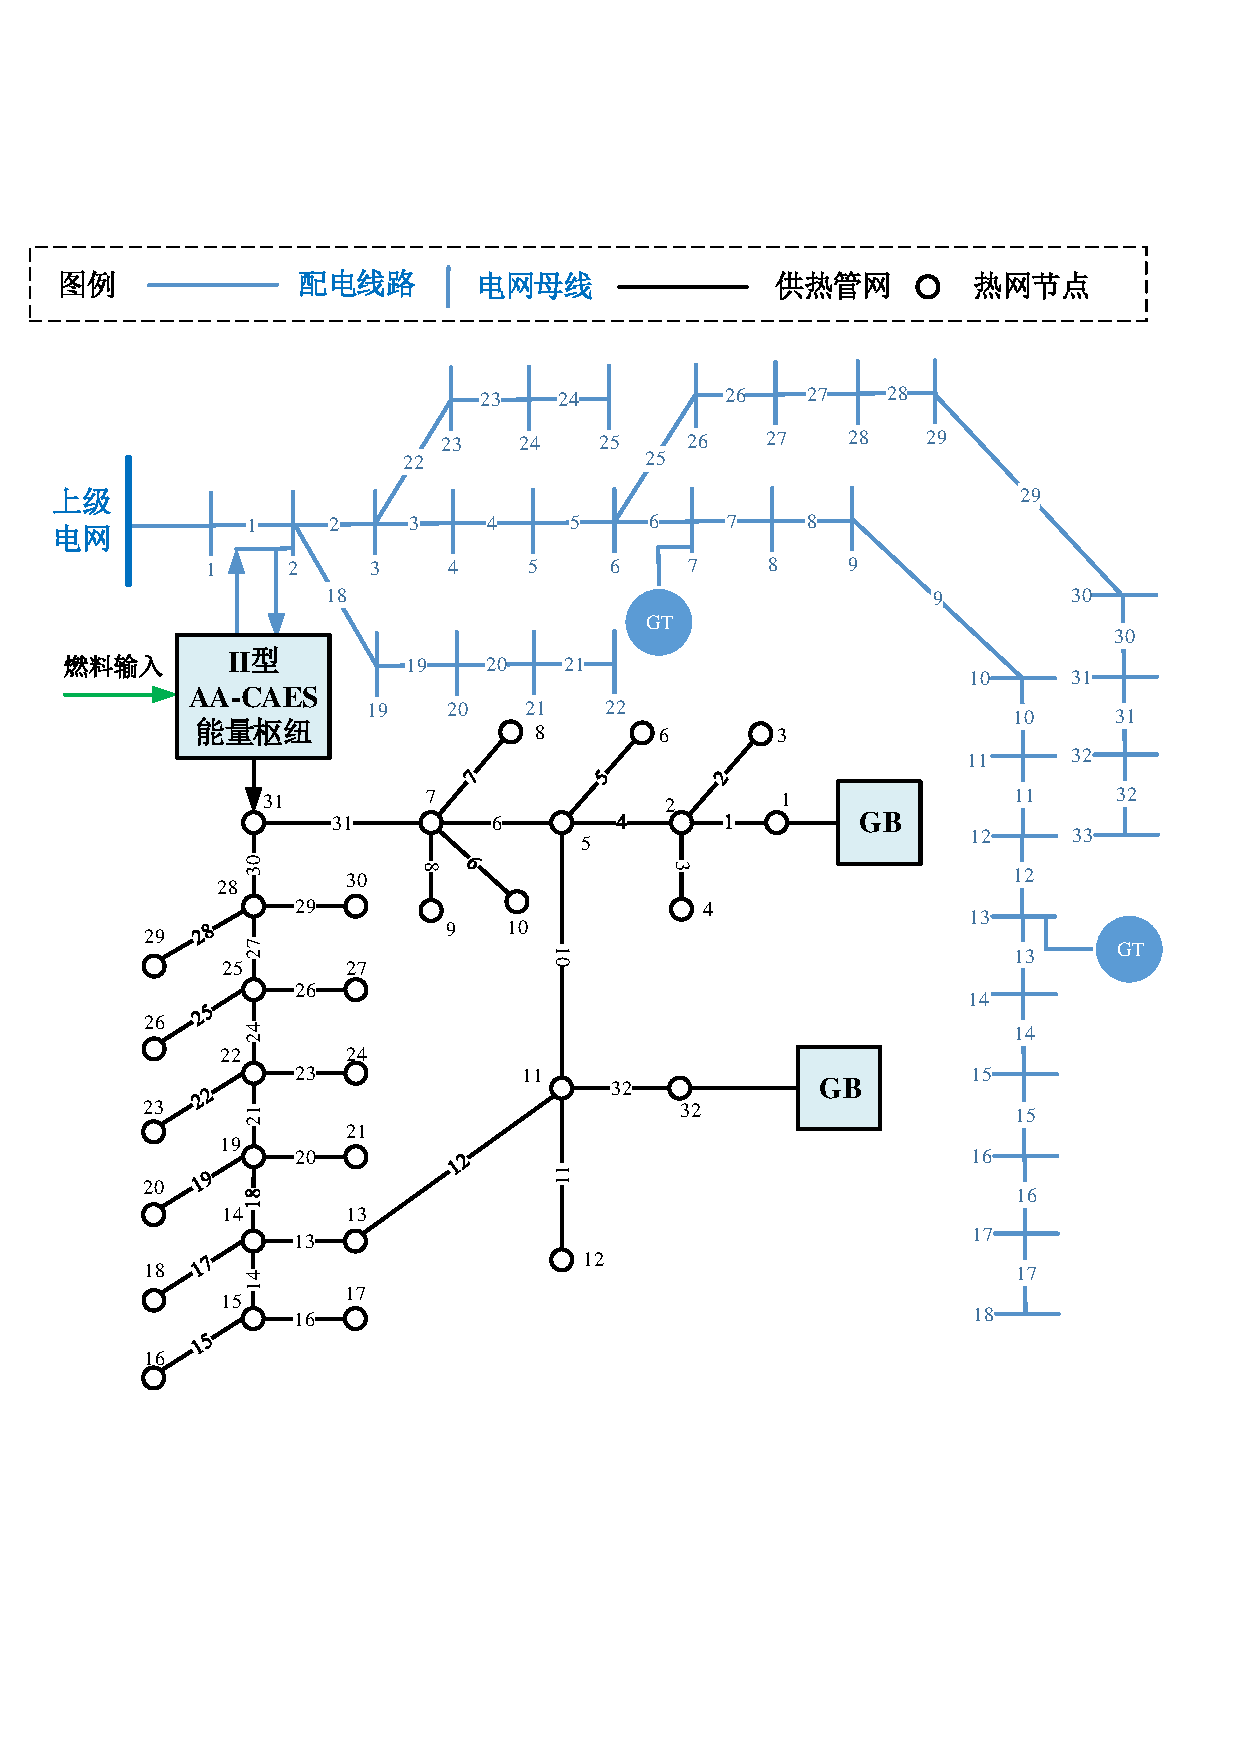
\includegraphics[scale=0.60]{figures/Chap4-10-EH-PDN-DHN-CN-V2.pdf}
\caption{独立运营环境下的区域热电综合能源测试系统}
\label{Fig:Chap4-EH-PDN-DHN-CN}
\end{figure}

\begin{table}[!htp]
\scriptsize
\renewcommand{\arraystretch}{1.3}
\renewcommand{\tabcolsep}{1em}
\caption{常规电源参数}
\centering
\begin{tabular}{ccccc}
\toprule
GT 编号 &$p^{g}$(MW) & $q^{g}$(MVar) & a($\$$/MW$^2$)&b($\$$/MW)\\
\midrule
 GT 1  &  [0, 1.5]  &  [0, 0.5]  &   0.12   &   20.0   \\
 GT 2  &  [0, 2.0]  &  [0, 1.0]  &   0.09   &   15.0   \\
\bottomrule
\end{tabular}
\label{tab:ParaGen-GT}
\end{table}

\begin{table}[!htp]
\scriptsize
\renewcommand{\arraystretch}{1.3}
\renewcommand{\tabcolsep}{1em}
\caption{常规热源参数}
\centering
\begin{tabular}{ccccc}
\toprule
GB 编号 &$h^{g}$(MW)& 位置& $\alpha$($\$$/MW$^2$) & $\beta$($\$$/MW)\\
\midrule
 GB 1  &  [0, 1.0]  &  节点 1    &   0.15   &   20.0   \\
 GB 2  &  [0, 1.0]  &  节点 32   &   0.16   &   18.0   \\
\bottomrule
\end{tabular}
\label{tab:ParaGen-GB}
\end{table}

\begin{table}[!htp]
\scriptsize
\renewcommand{\arraystretch}{1.3}
\renewcommand{\tabcolsep}{1em}
\caption{II型AA-CAES能量枢纽参数}
\centering
\begin{tabular}{ccccccccc}
\toprule
 变量   &  范围  & 单位 &  变量 &  范围 & 单位 & 变量 &  范围 & 单位 \\
\midrule
$p^{ch}$  & [0, 3.0] & MW & $E$ & [0, 10] & MWh &  $p^{gas}$ & [0, 1.5] & MW \\
$p^{dis}$ & [0, 2.0] & MW & $H$ & [0, 10] & MWh &  $p_0^g$   & [0, 3.0] & MW  \\
$h^{ch}$  & [0, 2.0] & MW & $p_m^{gb}$ & [0, 2.0] & MW & $h_m^b$ & [0, 1.5] & MW \\
$h^{dis}$ & [0, 1.5] & MW & $p_m^{db}$ & [0, 1.5] & MW & & &\\
\bottomrule
\end{tabular}
\label{tab:ParaHub}
\end{table}

\subsubsection{算例设置}
能量枢纽的竞标策略受到市场需求、能源价格、系统约束等多种因素影响,以为将针对不同的负荷曲线、配电零售电价、燃料价格、储能效率及系统限制等条件设置算例。

(1)不同的负荷曲线

我们考虑具有相同峰值负荷的不同季节热电需求曲线,如图~\ref{Fig:loadshape}~所示。其中,热需求在不同季节有较大差别,电需求在夏季由于空调负荷等的启动较高。

\begin{figure}[!t]
\centering
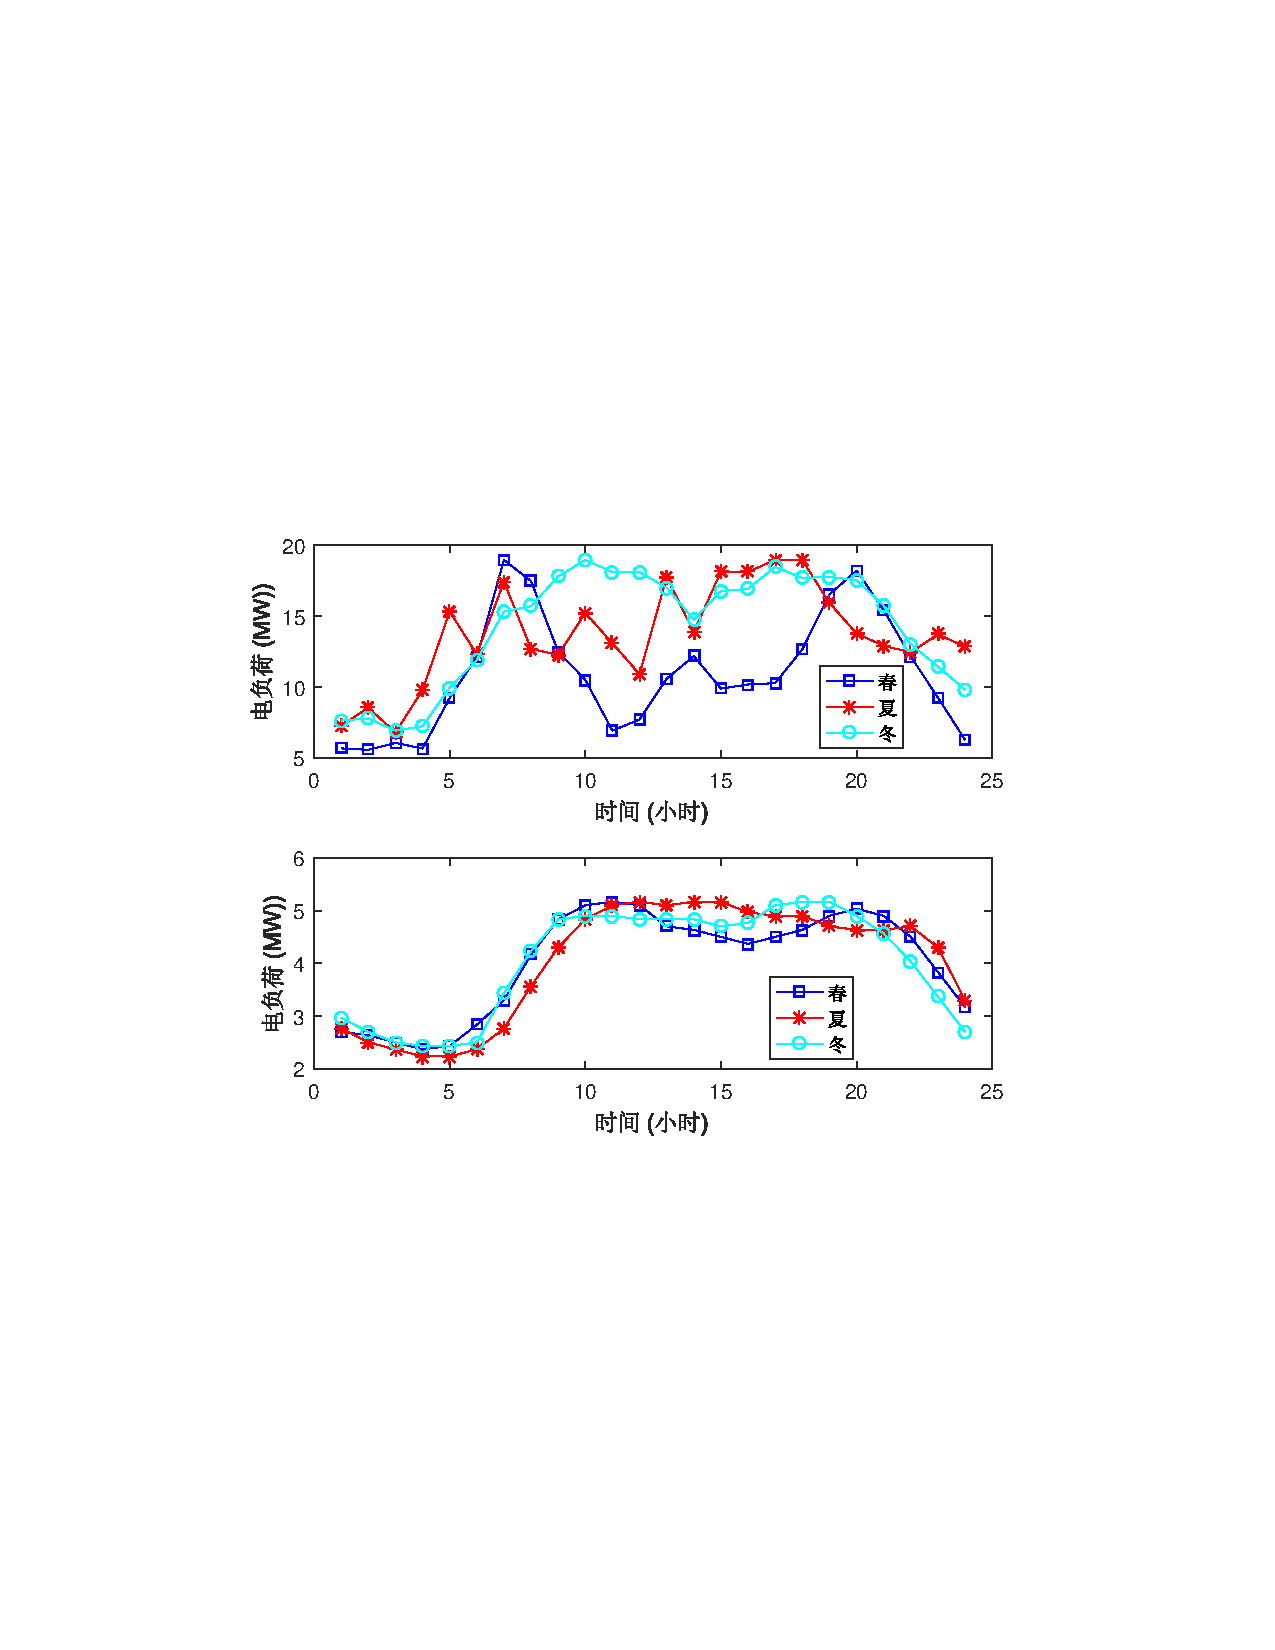
\includegraphics[scale=0.85]{figures/Chap4-6-LoadCurve.pdf}
\caption{典型季节热电负荷需求预测曲线}
\label{Fig:loadshape}
\end{figure}

(2)不同的配电零售电价

能量枢纽接入配电网的母线(Bus 2)处的电力零售价格是时变的。该零售价格由电力市场操作员EMO 提供,不依赖于能量枢纽及其它发电机组的调度。我们假定母线2可能存在四种零售电价曲线,分别为实时电价(El-RT)、分时电价(El-TOU)、峰谷差价(El-PV)以及电力市场中可能出现的价格波动大的极端情形(El-Ex),如图~\ref{Fig:GridPrice}~ 所示。

\begin{figure}[!htp]
\centering
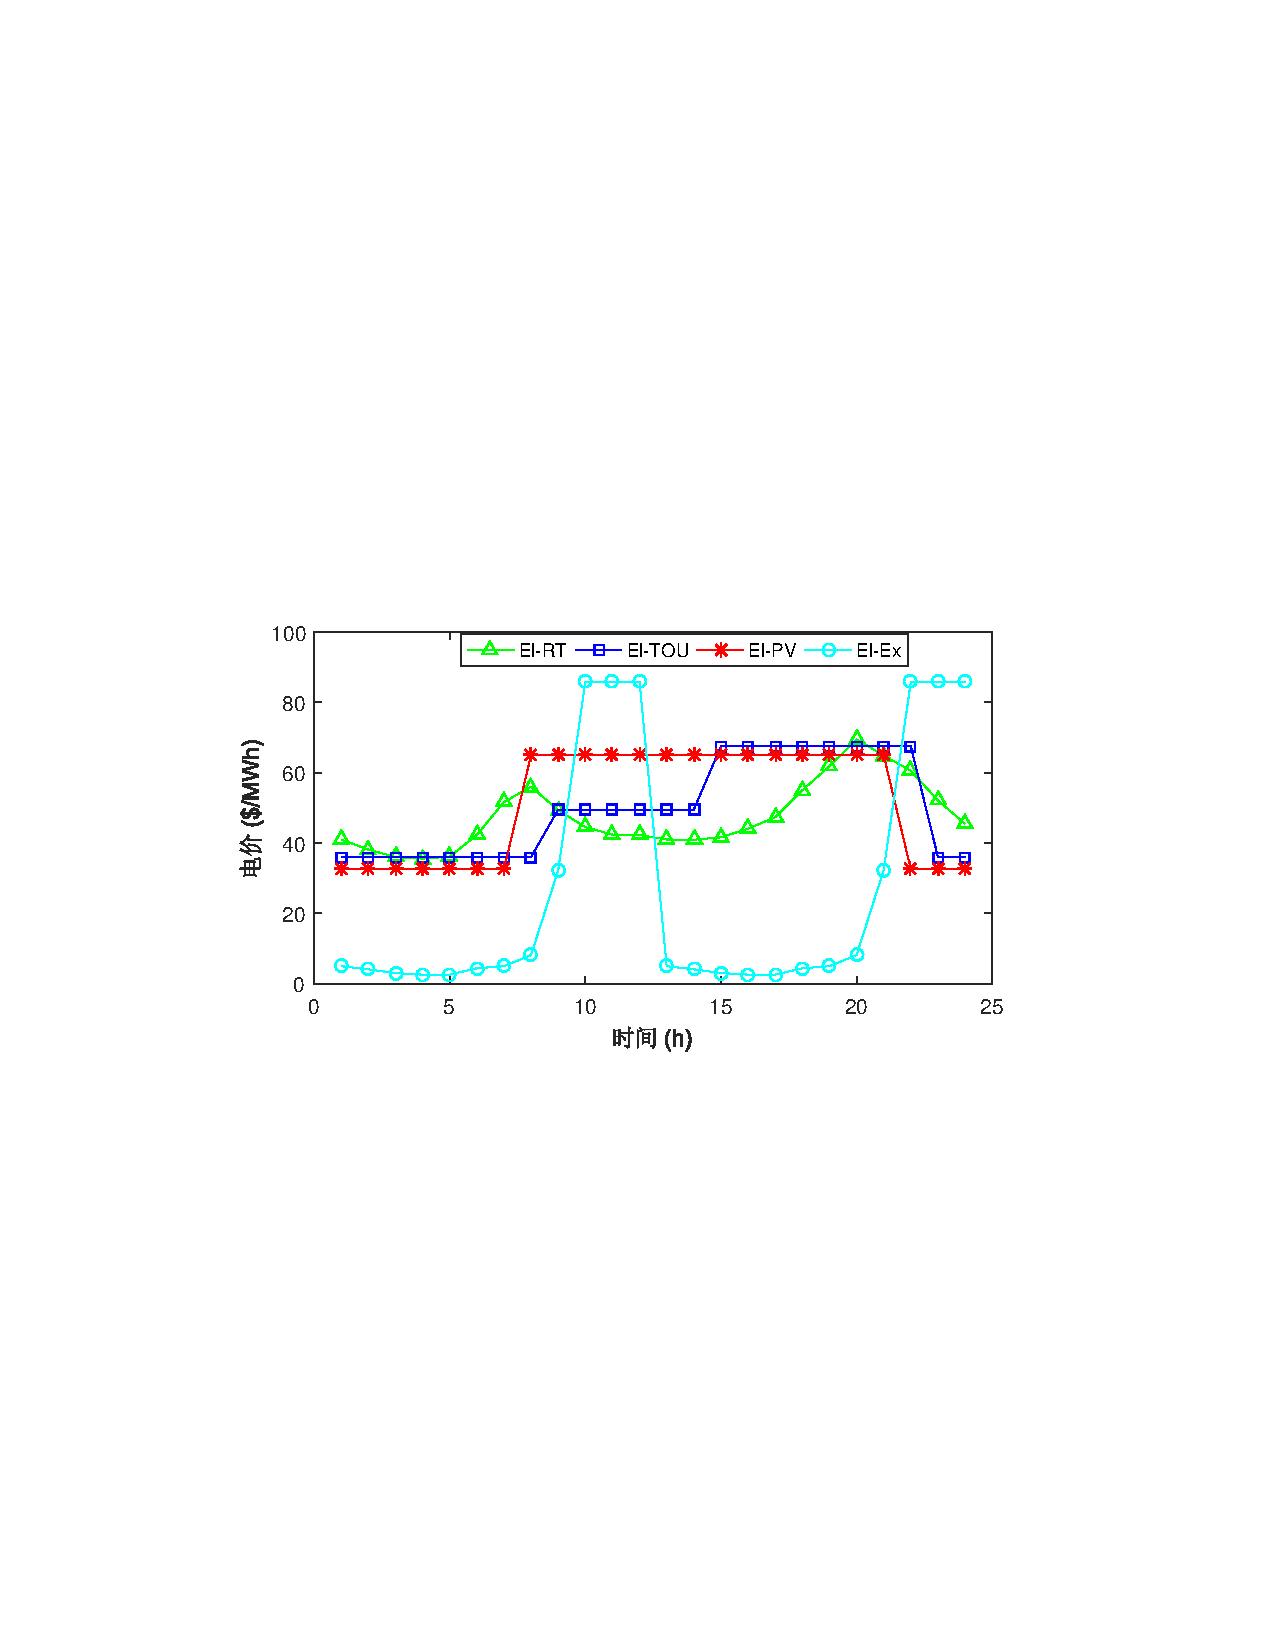
\includegraphics[scale=0.80]{figures/Chap4-7-ELPrice.pdf}
\caption{馈线入口母线电价曲线}
\label{Fig:GridPrice}
\end{figure}

(3)不同的燃料价格

我们假定燃料价格由能量枢纽与外部燃料市场协议决定,该值可以为固定值或时变值。我们考虑三种不同的燃料价格机制:1)基准算例BEN中$\gamma = 26 \$/$MWh且保持不变;2)极端情形算例Gas-Ex 中$\gamma = 40 \$/$MWh且保持不变;3)在燃气价格峰谷机制算例Gas-PV中,在时段7-18取$\gamma = 30 \$/$MWh,在其它时段$\gamma = 20 \$/$MWh。

(4)不同的储能效率

能量枢纽内部实行多能流时空搬移的储能单元的效率对其竞标策略具有较大的影响。对于AA-CAES而言,其循环效率依赖于不同的结构形式及对应实现形式的成熟度,典型电- 电效率为40$\%$-70$\%$ \cite{CAES-Reserve-11},采用高温储热、外部光热辅助等方案后其效率可达75$\%$-85$\%$ \cite{A-CAES-Dynamic-17,AA-CAES-Demo-ALACAES-1,AA-CAES-Demo-ALACAES-2,ST-CAES-CXT-18}。 对于能量枢纽内部的储热单元,其循环效率通常可达98$\%$ \cite{TES-CSP-review-13}。 因此,我们将在保持储热效率($\eta_{+}^{tsu}/\eta_{-}^{tsu}$)为 98$\%$时,将AA-CAES的压缩储能与膨胀释能效率($\eta_{+}^{esu}/\eta_{-}^{esu}$) 从90$\%$ 降至 60$\%$ (对应于循环效率从81$\%$ 降至 36$\%$)来研究储电效率对热电能量枢纽竞标策略的影响。

(5)市场力测试与限制

能量枢纽具有一定的市场力,其竞标策略将对电力市场与热力市场的出清结果具有影响。一般地,若能量枢纽的售电电价或售热热价低,EMO与HMO倾向于从能量枢纽购买更多的电能或热能;反之,若能量枢纽售电电价或售热热价过高,市场调度员会选择其它电源或热源来满足负荷需求,导致能量枢纽失去一定的市场份额。有时,由于配电线路或供热管道阻塞或其它运行安全等系统因素的影响,调度员不得不从能量枢纽购买电能或热能。因此,为了测试与限制能量枢纽的市场力,我们将分析:1)算例~MP-RtCap~,配电网馈线容量从~3~MW 调整至 ~6~MW;2)算例MP-TBPos,将GT1 与 GT2分别移动至母线6与母线13,同时增加其功率上界至2MW;3)算例MP-GasLim:将燃料市场输入上界从1.5MW 降至1MW。

\subsubsection{通用设定及模型求解}

在本节的所有算例中,采用~128~段离散化能量枢纽在各个市场的报价,即布尔展开法中~$K=7$~。出于网络安全等考虑,从上级电网(电力批发市场)馈入配电网的电功率~($p_0^g$)~ 上界(即馈入节点容量)为~3MW,能量枢纽从燃料市场获取的燃气输送率~($p^{gas}$)~最大为~1.5 MW。同时,假定能量枢纽与热力市场协议后决定的热价竞标标的~($\zeta^b$)~的最小值、最大值及平均值分别为~12\$/MWh, 30\$/MWh 及 25 $\$$/MWh。此外,假定能量枢纽从电力市场的购电电价标的($\chi^b$) 不低于母线~2~在$t$时刻的电力零售价,以及能量枢纽向电力市场的售电电价标的($\xi^b$)不高于当日电价峰值的~1.25~倍。

能量枢纽内部AA-CAES的压缩、膨胀效率~($\eta_+^{esu}/\eta-^{esu}$)~设为~90$\%$,储热单元的充、放效率($\eta_+^{tsu}/\eta-^{tsu}$)亦设为~98$\%$。热泵的热效率($\eta^{hp}$)设为3,(背压式)CHP~的电热生产效率($\eta_e^{chp}/\eta_h^{chp}$)分别设为0.35与0.65。算例与负荷及价格曲线对应关系见附录~\ref{cha:aa-caes-case-append},其它算例将在分析部分进行具体解释说明。

本节所有的计算采用YALMIP\cite{YALMIP}建模,并调用CPLEX 求解器完成,硬件配置为Intel i5-4210M CPU 及 16GB RAM\footnote{本节代码可参见https://github.com/AIRicky/Energy-Hub-Market-Operation}。各算例下的收益与~50~次运行平均计算时间如表\ref{tab:Results}所示,计算时间基本为分钟级,对于日前综合能源市场的运行而言是可接受的。
\begin{table}[!htp]
\scriptsize
\renewcommand{\arraystretch}{1.3}
\renewcommand{\tabcolsep}{0.83em}
\caption{各算例竞标收益 (\$)与计算时间 (s)}
\centering
\begin{tabular}{ccccccc}
\toprule
{场景} & {PDN 成本} & {Gas 成本} & {PDN 收入} & {DHN 收入} & {总利润} & {计算时间}\\
\midrule
BEN      & 278.28 & 598.57   & 951.66   &  394.68  & 469.48  & 231.2\\
EI-TOU   & 331.07 & 489.72   & 993.02   &  397.77  & 569.99  & 62.03\\
El-PV    & 303.23 & 774.96   & 1365.0   &  396.08  & 682.88  & 88.97\\
El-Ex    & 152.30 & 519.09   & 1178.4   &  396.36  & 903.39  & 85.61\\
Spring   & 324.41 & 680.61   & 1106.4   &  378.50  & 479.91  & 197.5\\
Summer   & 301.03 & 538.06   & 947.67   &  309.94  & 418.53  & 28.83\\
%Fall     & 301.03 & 587.60   & 947.67   &  394.68  & 453.73  & \textcolor{blue}{706.4}\\
Gas-Ex   & 381.41 & 134.54   & 426.12   &  393.79  & 303.95  & 42.77\\
Gas-PV   & 309.14 & 360.00   & 831.99   &  393.79  & 556.64  & 103.9\\
\bottomrule
\end{tabular}
\label{tab:Results}
\end{table}

\subsubsection{基准算例分析}

基准算例(BEN)下,II型AA-CAES能量枢纽向电力及热力市场的竞标标的如图~\ref{Fig:BAUCase}~所示,能量枢纽内部AA-CAES与储热单元的~SOC~\footnote{此处的储热SOC不是AA-CAES内部储热单元的SOC,其与此处的储电SOC具有相同形状,在设计时予以考虑,实现压力势能与压缩热能的匹配。}变化如图~\ref{Fig:ESSTES}~所示。能量枢纽在时段1-6以较低的电价从配电网中购入电能,其中一部分存储于能量枢纽内部的AA-CAES,以供用电高峰(高价)时段(如时段7-8、时段19-23)实现套利运行。同时,区域热网的峰值负荷为~2~MW,仅靠锅炉~GBs~难以满足峰值热负荷的需求,因此能量枢纽可以维持一定量的热能输出。在时段1-5,由于电价便宜,能量枢纽不从燃气市场购买燃料,其对外输出的热能主要通过能量枢纽内部的热泵靠消耗电能提供。在时段3 与时段5,更多热能从热泵转化,并存储于能量枢纽内部的储热单元中,以供其它时段使用。

\begin{figure}[!t]
\centering
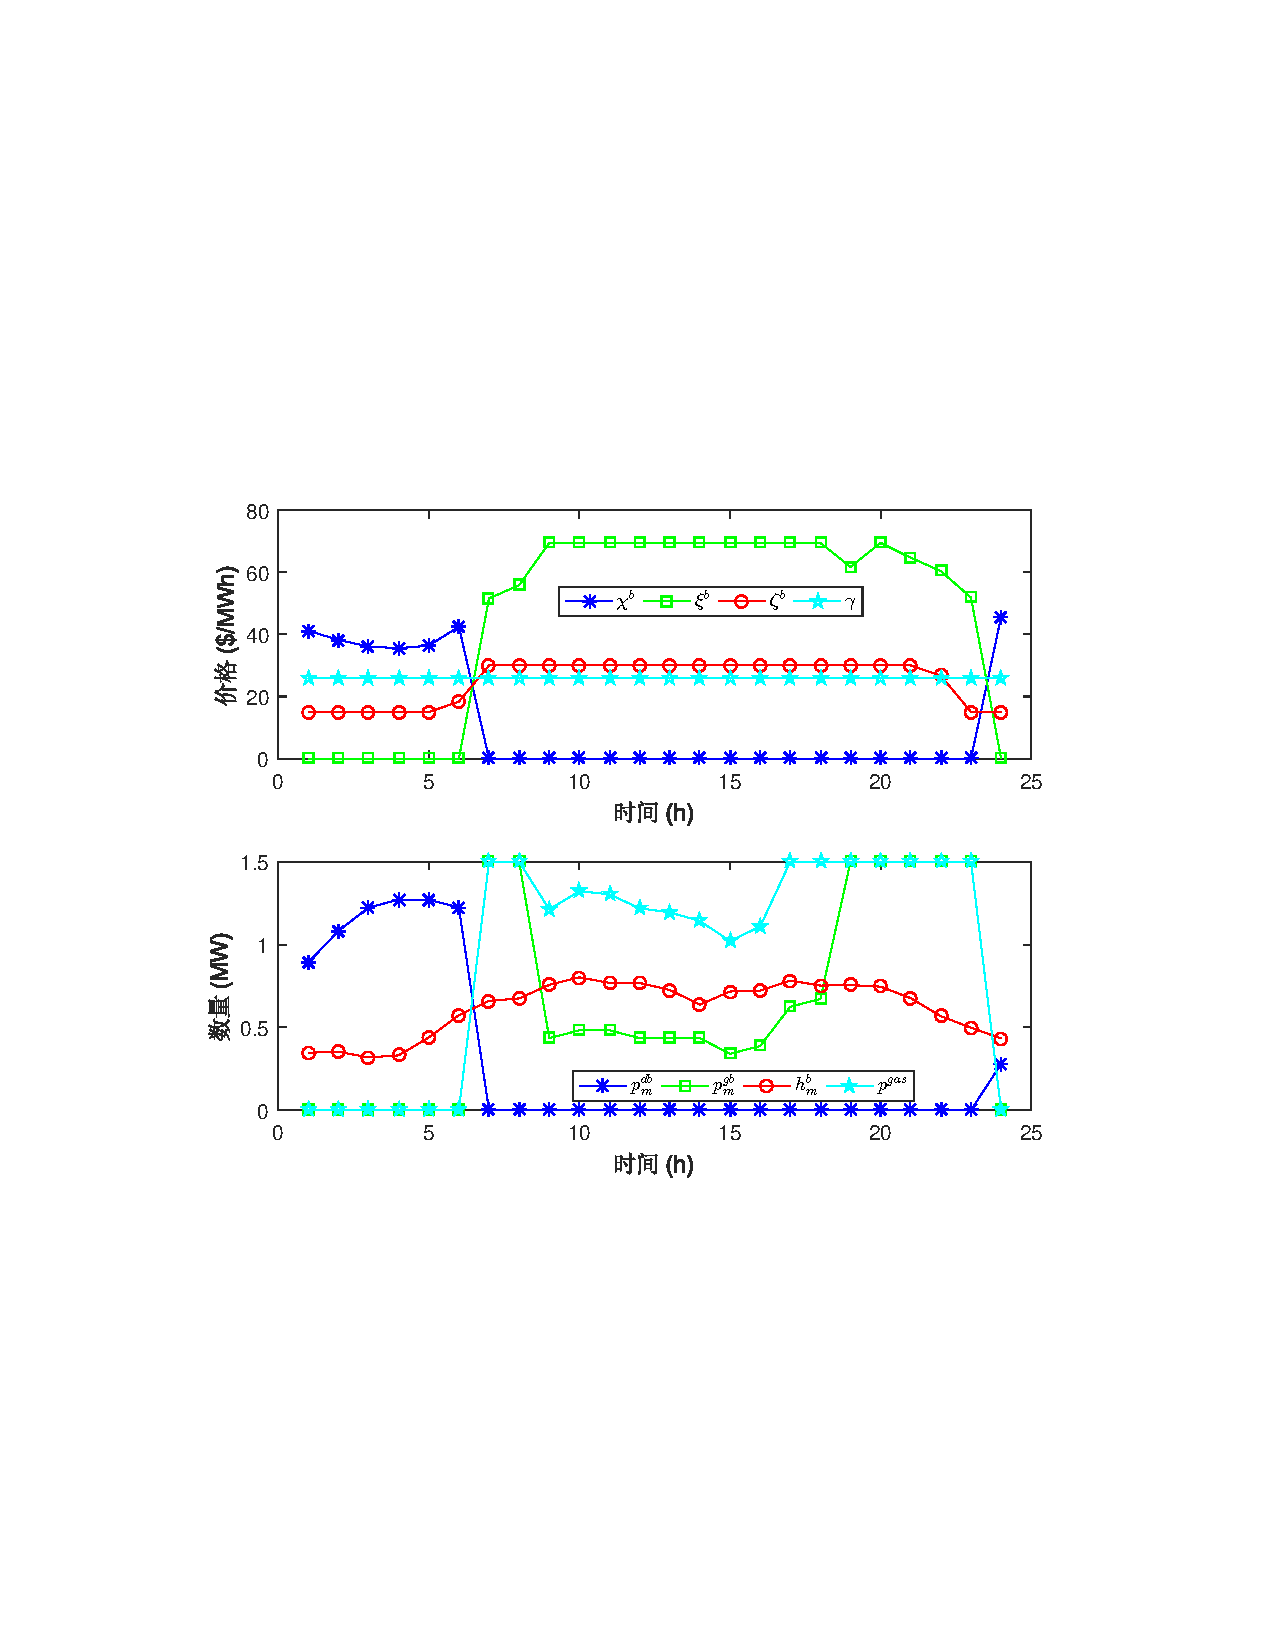
\includegraphics[scale=0.75]{figures/Chap4-8-BENBid.pdf}
\caption{算例~BEN~中价格与电量竞标标的}
\label{Fig:BAUCase}
\end{figure}

从时段~6~开始,实时电价开始升高,能量枢纽转向购买燃气通过~CHP~生产热能与电能。由于热泵较~CHP~具有更高的效率,时段~1-5~能量枢纽的售热热价~$\zeta^b$~比该天其它时段的报价低,其它时段的热能主要通过~CHP~消耗燃料提供。此外,能量枢纽的售购电量~($p_{m}^{gb}, p_{m}^{db}$)~ 及售热量标的~($h_{m}^b$)~与两个市场出清值相同。通过在热力市场、电力市场及燃料市场的综合交叉套利运行,在BEN算例情形下,能量枢纽的净利润达~$\$469.48$。
\begin{figure}[!t]
\centering
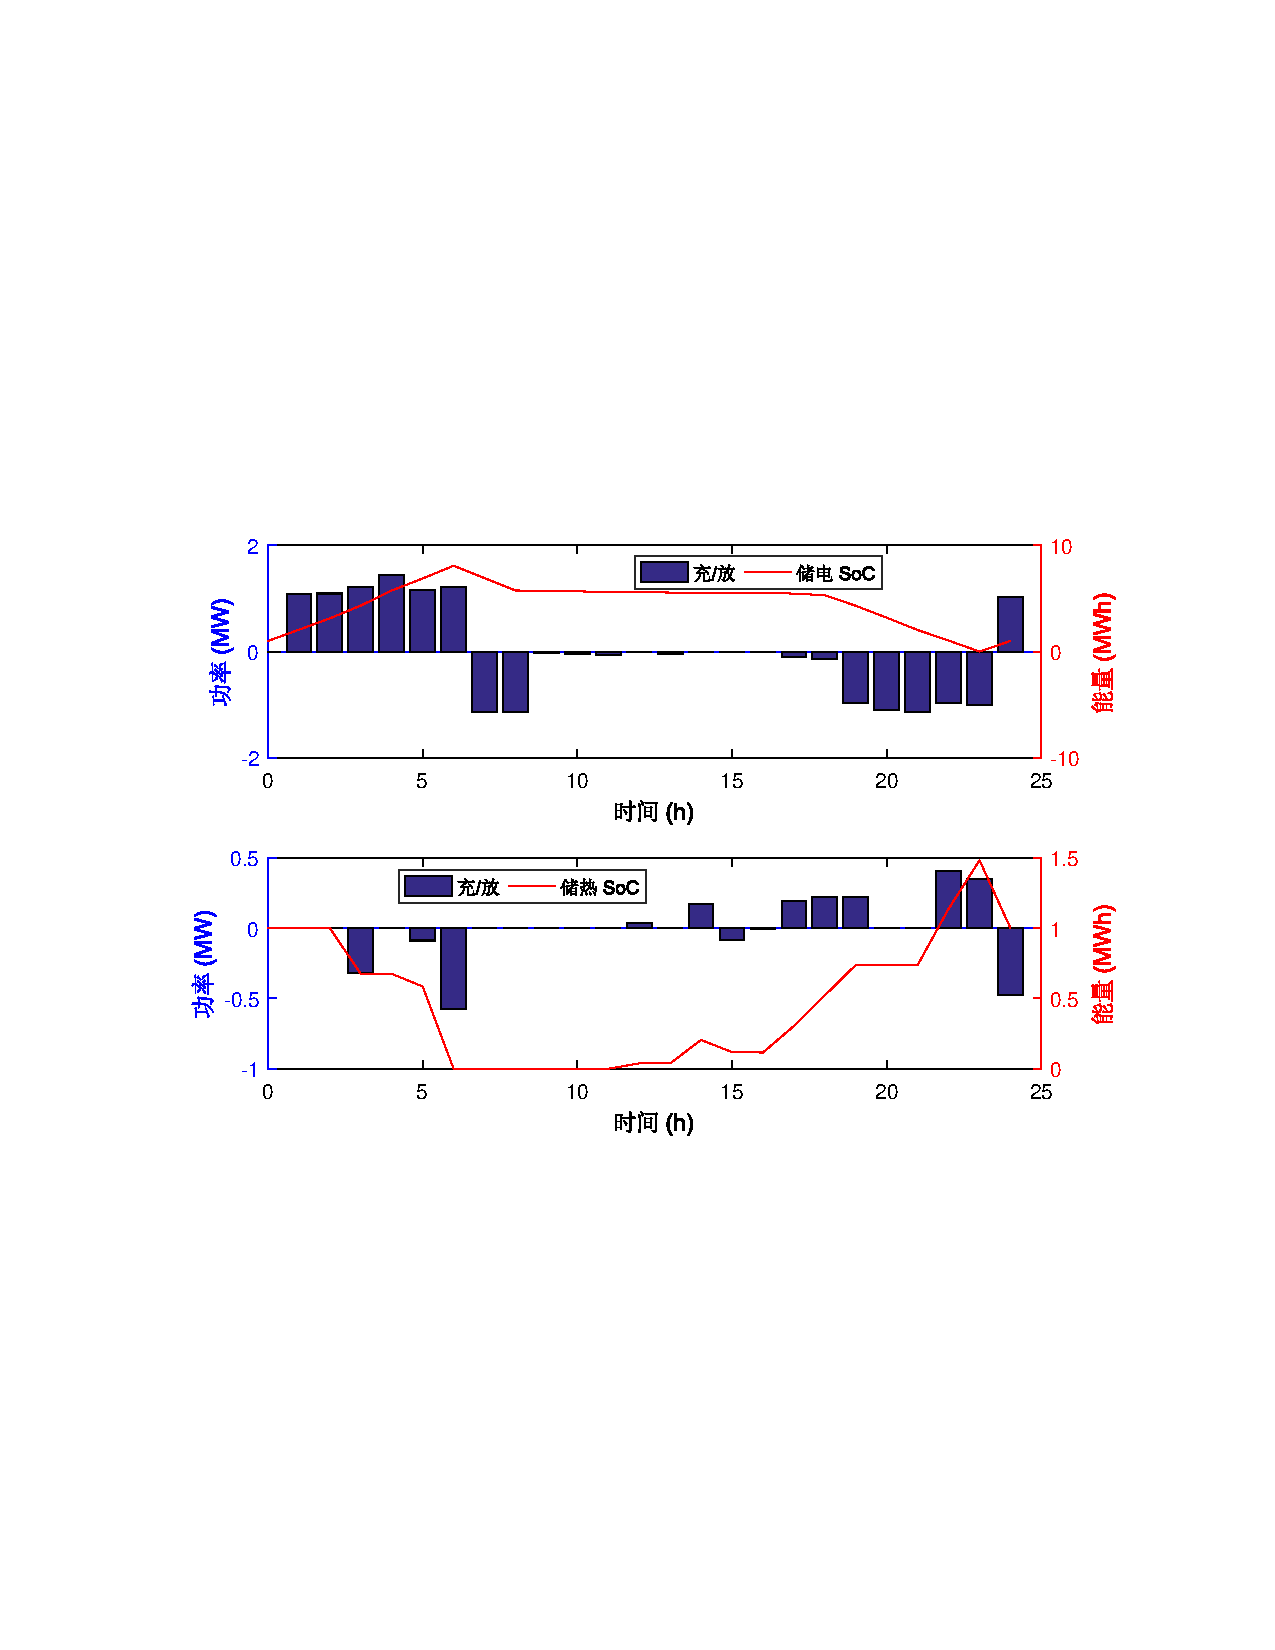
\includegraphics[scale=0.78]{figures/Chap4-9-ESSTESBAU.pdf}
\caption{能量枢纽内部储热与储电单元~SOCs~}
\label{Fig:ESSTES}
\end{figure}

\subsubsection{电价与燃料价格的影响}
配电电力市场的电价机制和天然气市场的燃料价格对AA-CAES型能量枢纽在热电能流市场的竞标策略有着重要的影响,算例{BEN}、{Gas-PV}及{Gas-Ex}下能流枢纽的燃气购买量如图\ref{Fig:GasInGasPrice}所示。可以发现,算例{Gas-Ex}中当燃气价格从~26$\$$/MWh~增加到~40$\$$/MWh~时,能量枢纽转向从电力市场购买更多的电力,不同于算例{BEN} 中在高峰时刻购买燃气以满足负荷需求,此时能量枢纽的运行策略为通过消耗电能产生足够的热能,并存贮于能量枢纽内部的储热单元。随着综合能源系统中电、气、热的深度融合,未来将有可能出现实时燃气市场,届时能量枢纽将会有更大的运行灵活性。

\begin{figure}[!htp]
\centering
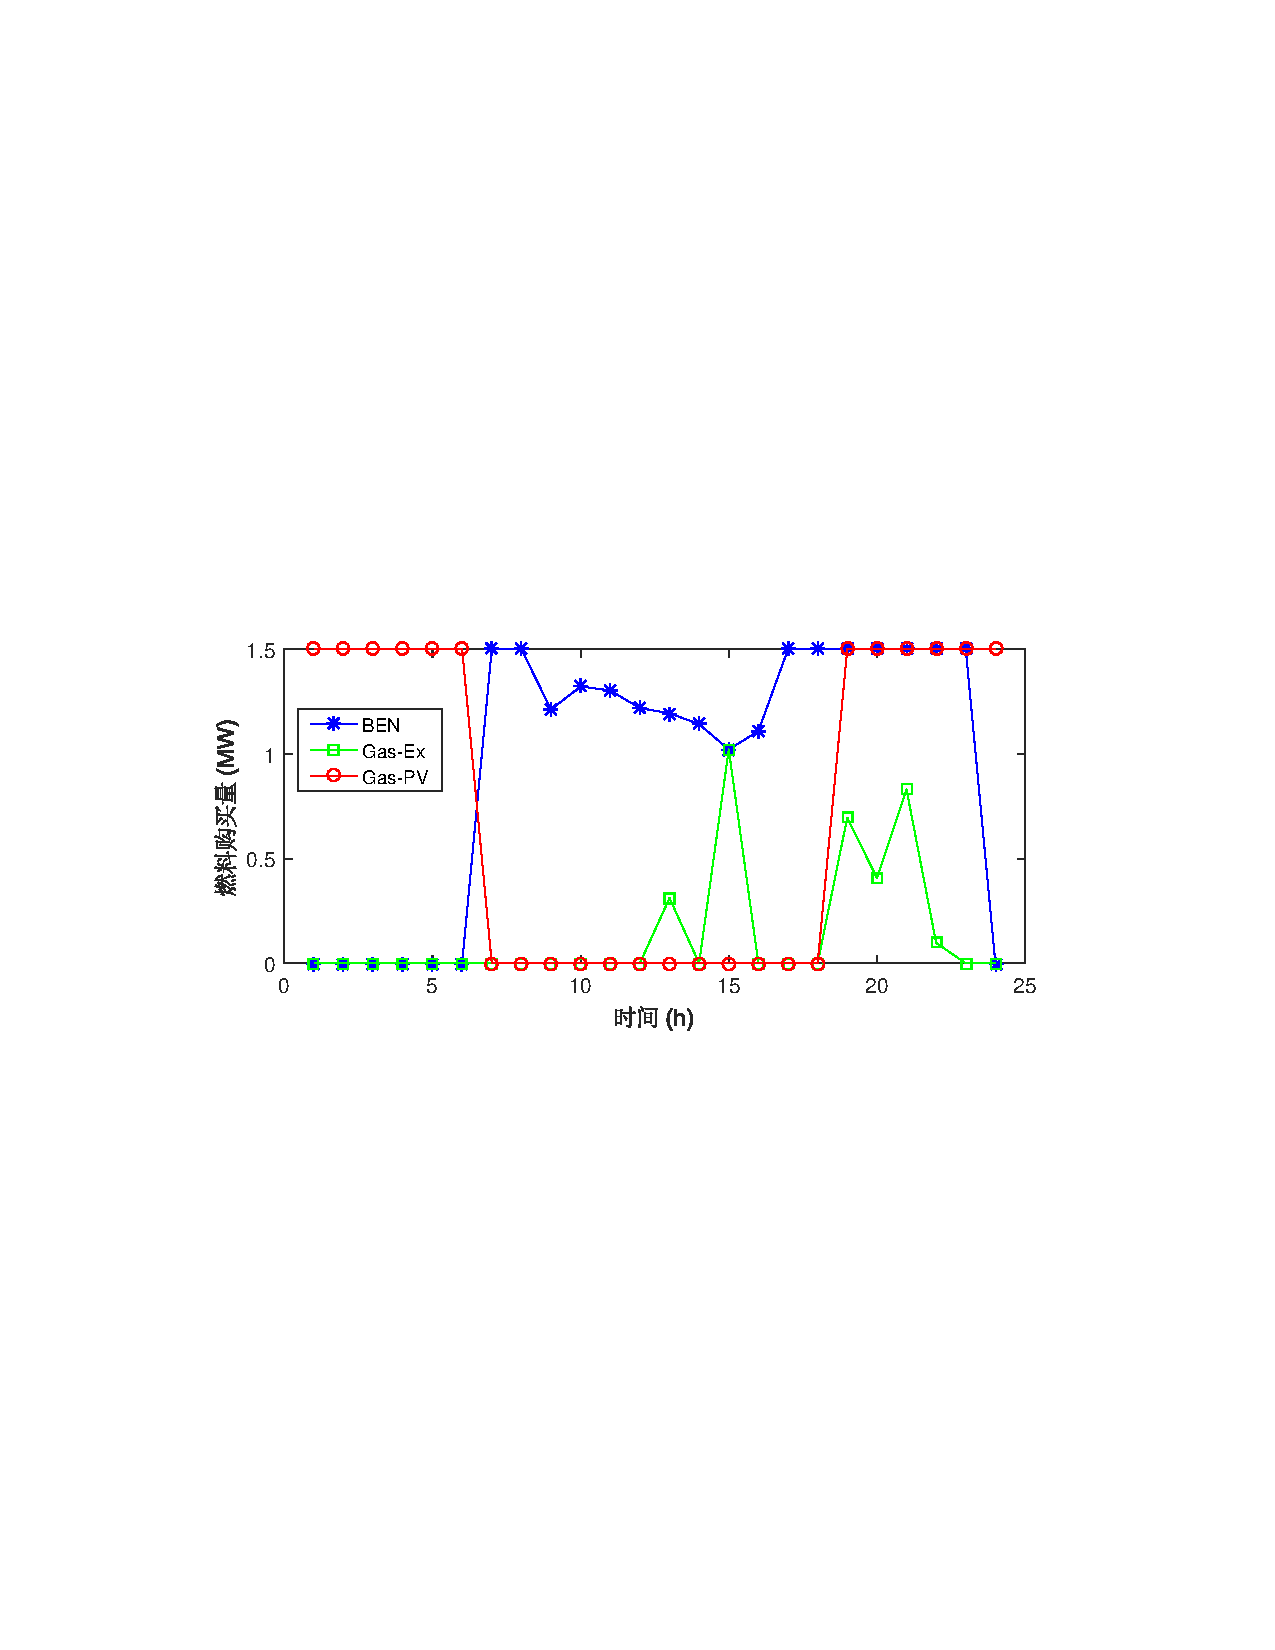
\includegraphics[scale=0.75]{figures/Chap4-12-GasIn_GasPrice.pdf}
\caption{不同燃料价格下的购气量对比}
\label{Fig:GasInGasPrice}
\end{figure}

从图\ref{Fig:GasInGasPrice}中可以看到,由于燃料价格较低,在算例{Gas-PV}中能量枢纽购入的燃料多于算例{Gas-Ex}。同时,由于燃料价格低导致的~CHP~生产成本低,能量枢纽从电力市场获得了更多收益。与算例{BEN}相比,算例{Gas-PV}的燃料购买成本较低,其原因在于在负荷低谷时期购买了燃料,从而导致算例{Gas-PV}的收入最高。当然,上述分析结论并非通用,而是依赖于实际的价格曲线。

图\ref{Fig:PriceBidComp}与图\ref{Fig:HeatPriceElPrice}分别给出了在算例{El-TOU},{El-PV}及{El-Ex}中能量枢纽在电力市场的售购电价竞标标的与在热力市场的售热热价竞标标的。算例{El-Ex}中,在时段1-6 能量枢纽向电力市场提交最低的售电电价($\xi^b$),在时段8-24能量枢纽向热力市场提交最高的售热热价($\chi^b$), 进而获得了最高的套利收益$\$1178.4$ 以及最高的运行利润$\$903.39$。

\begin{figure}[!htp]
\centering
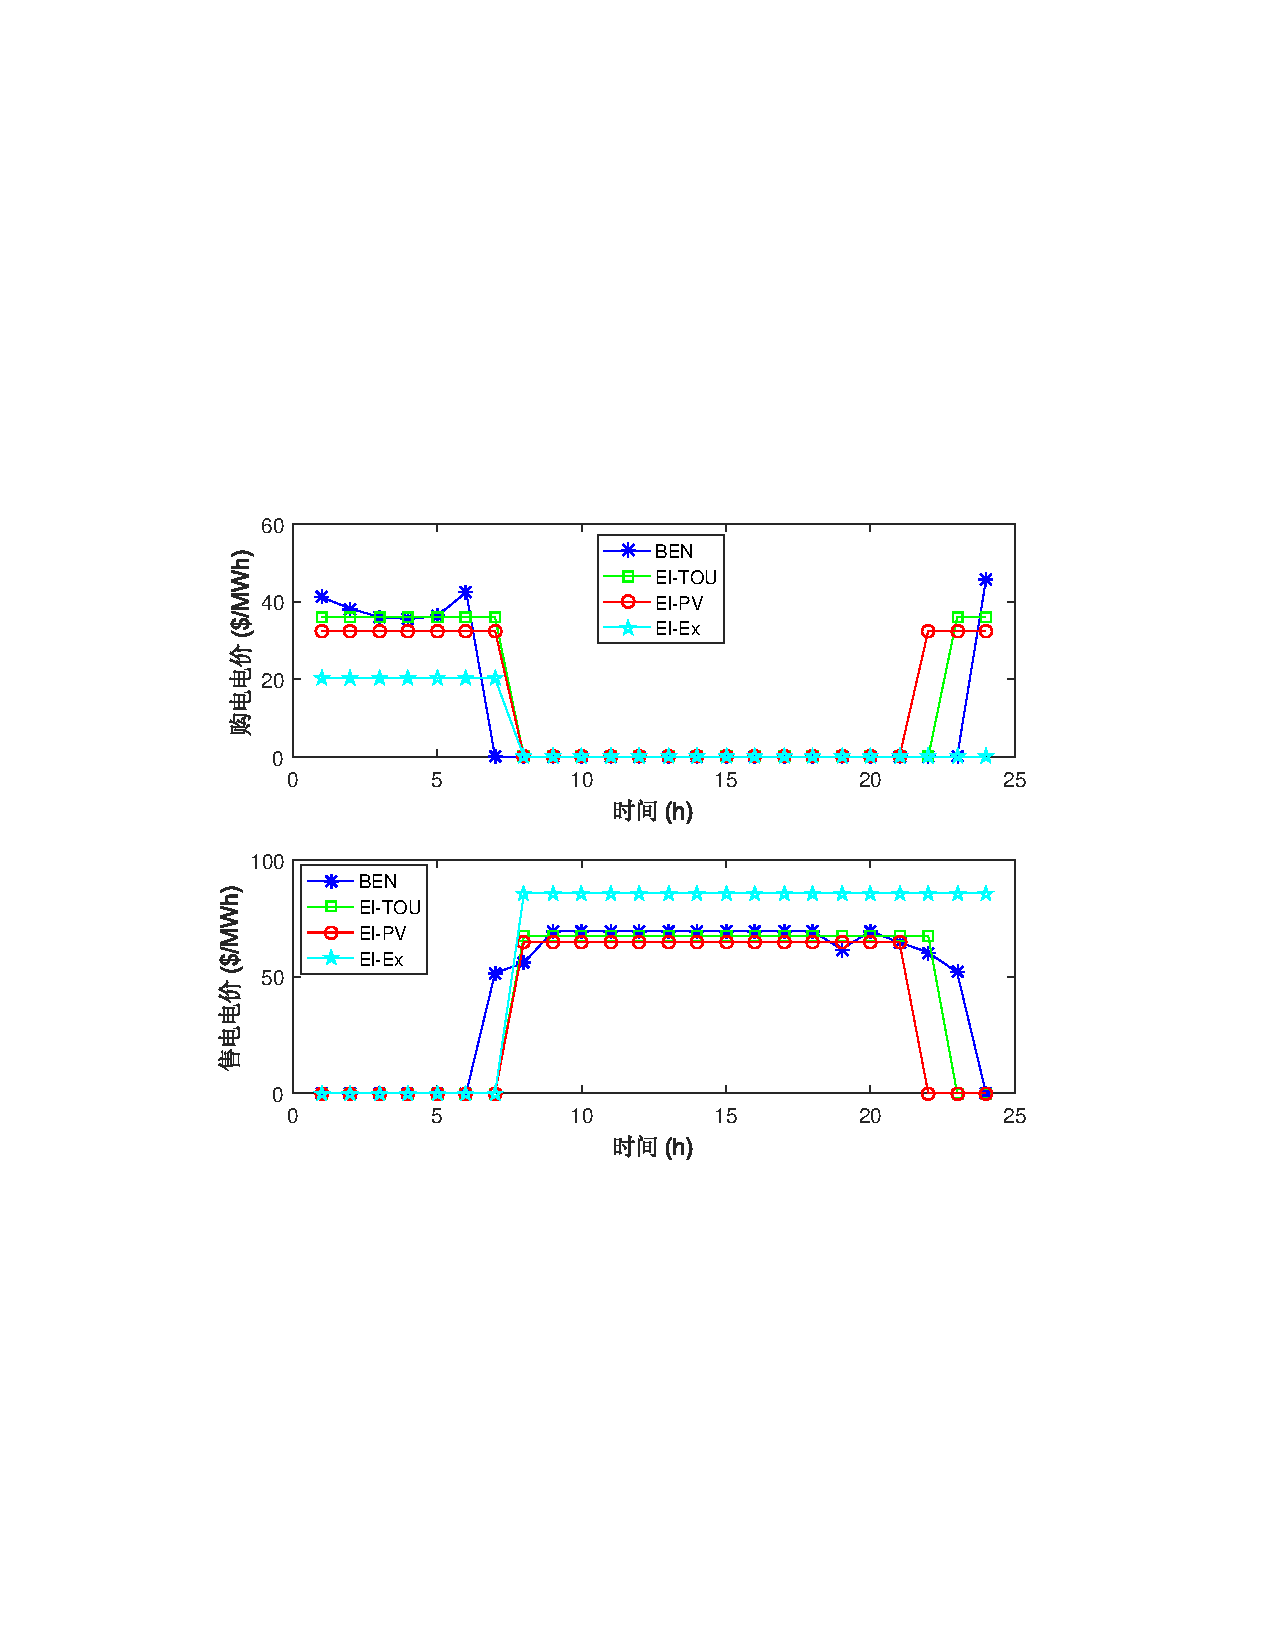
\includegraphics[scale=0.76]{figures/Chap4-10-ComparePrice.pdf}
\caption{各电价机制下能量枢纽上报于电力市场的竞标售/购电价}
\label{Fig:PriceBidComp}
\end{figure}

\begin{figure}[!htp]
\centering
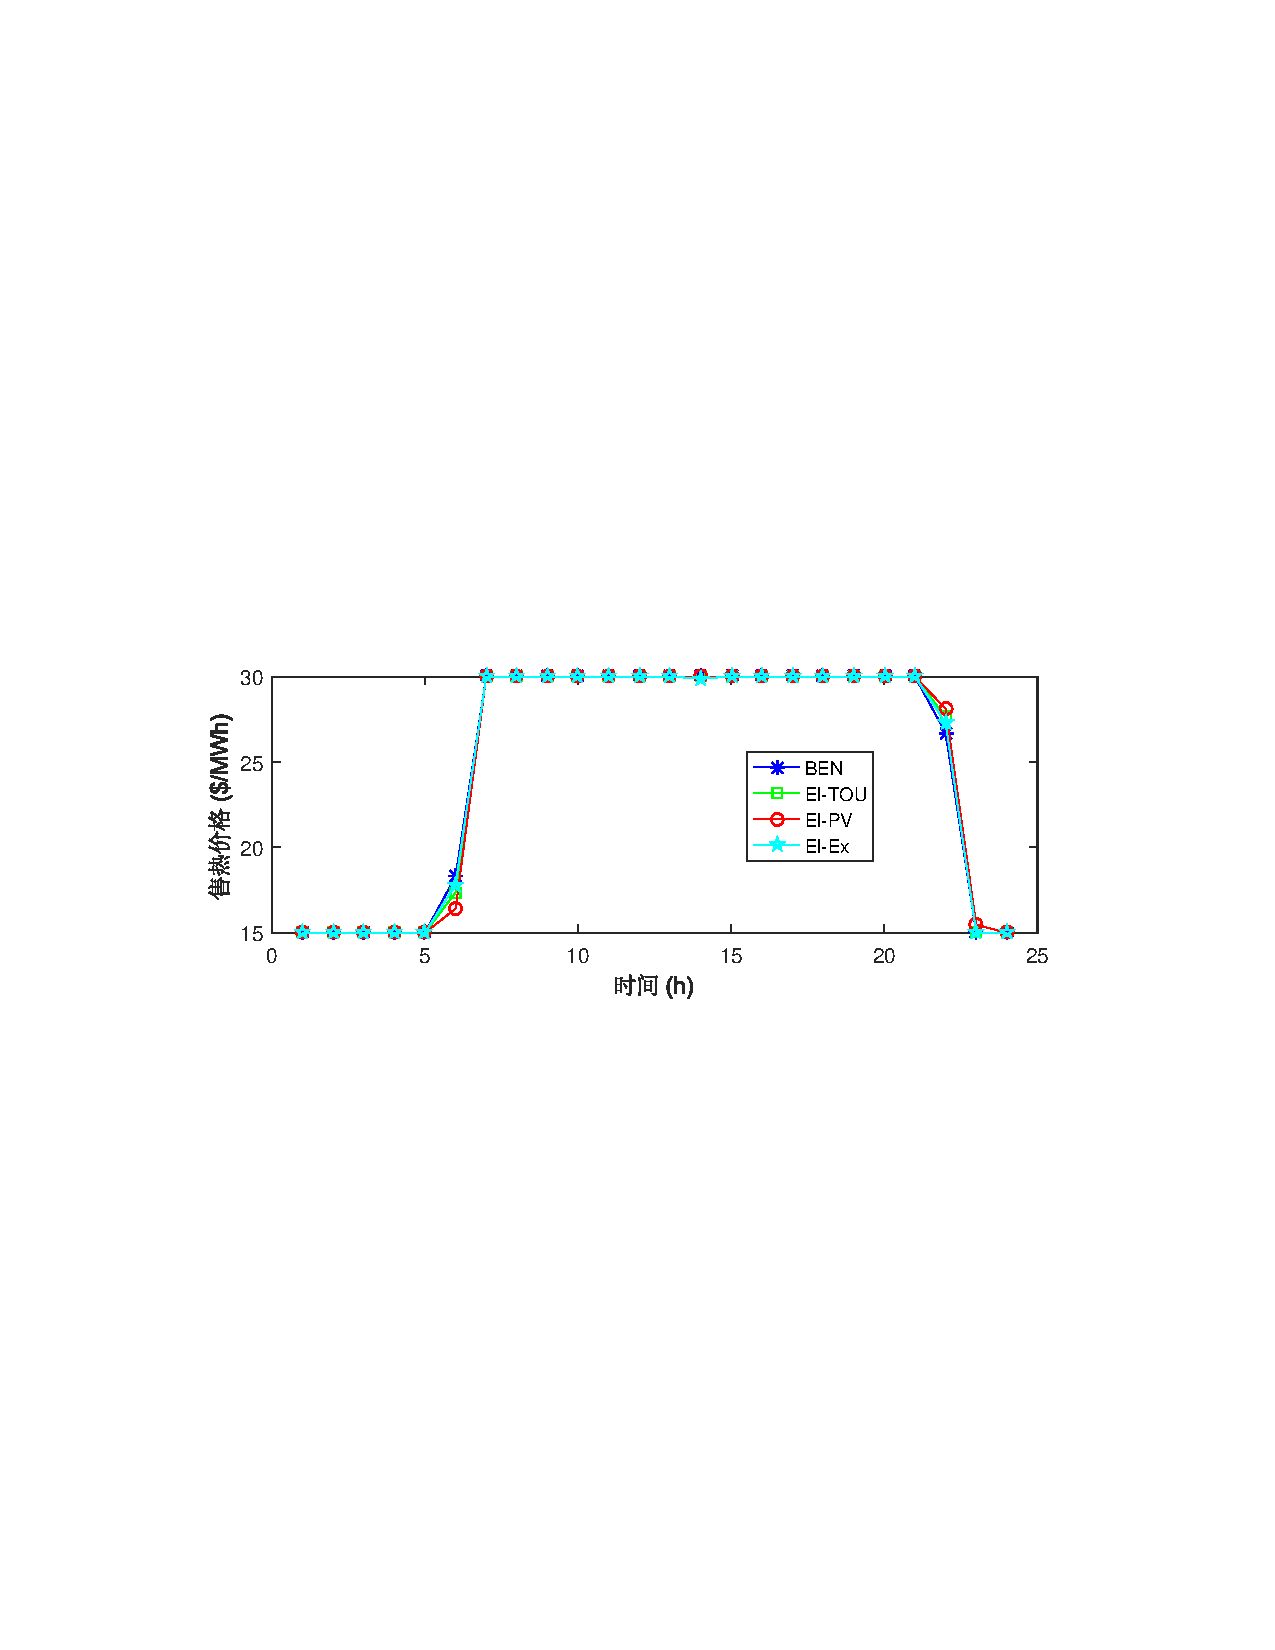
\includegraphics[scale=0.75]{figures/Chap4-11-HeatPriceElPrice.pdf}
\caption{各电价机制下能量枢纽上报于热力市场的售热热价}
\label{Fig:HeatPriceElPrice}
\end{figure}

由图\ref{Fig:HeatPriceElPrice}可知,电力市场采用的电价机制对II型AA-CAES热电能量枢纽在热力市场的竞标热价的影响不大,其主要原因在于在时段7-21,热负荷需求较高,因此作为所研究的供热网络中比不可少的热源之一,能量枢纽具有一定的市场力,其供热价格竞标标的达到允许的上界。

\subsubsection{负荷特性的影响}
图~\ref{Fig:HeatBidComp}~给出了基准算例~BEN~(冬季)与算例夏季中能量枢纽在热力市场的竞标标的。由于夏季的热负荷需求比冬季少,能量枢纽通过向~DHN~出售热力获取的收益将小于基准算例BEN。

\begin{figure}[!htp]
\centering
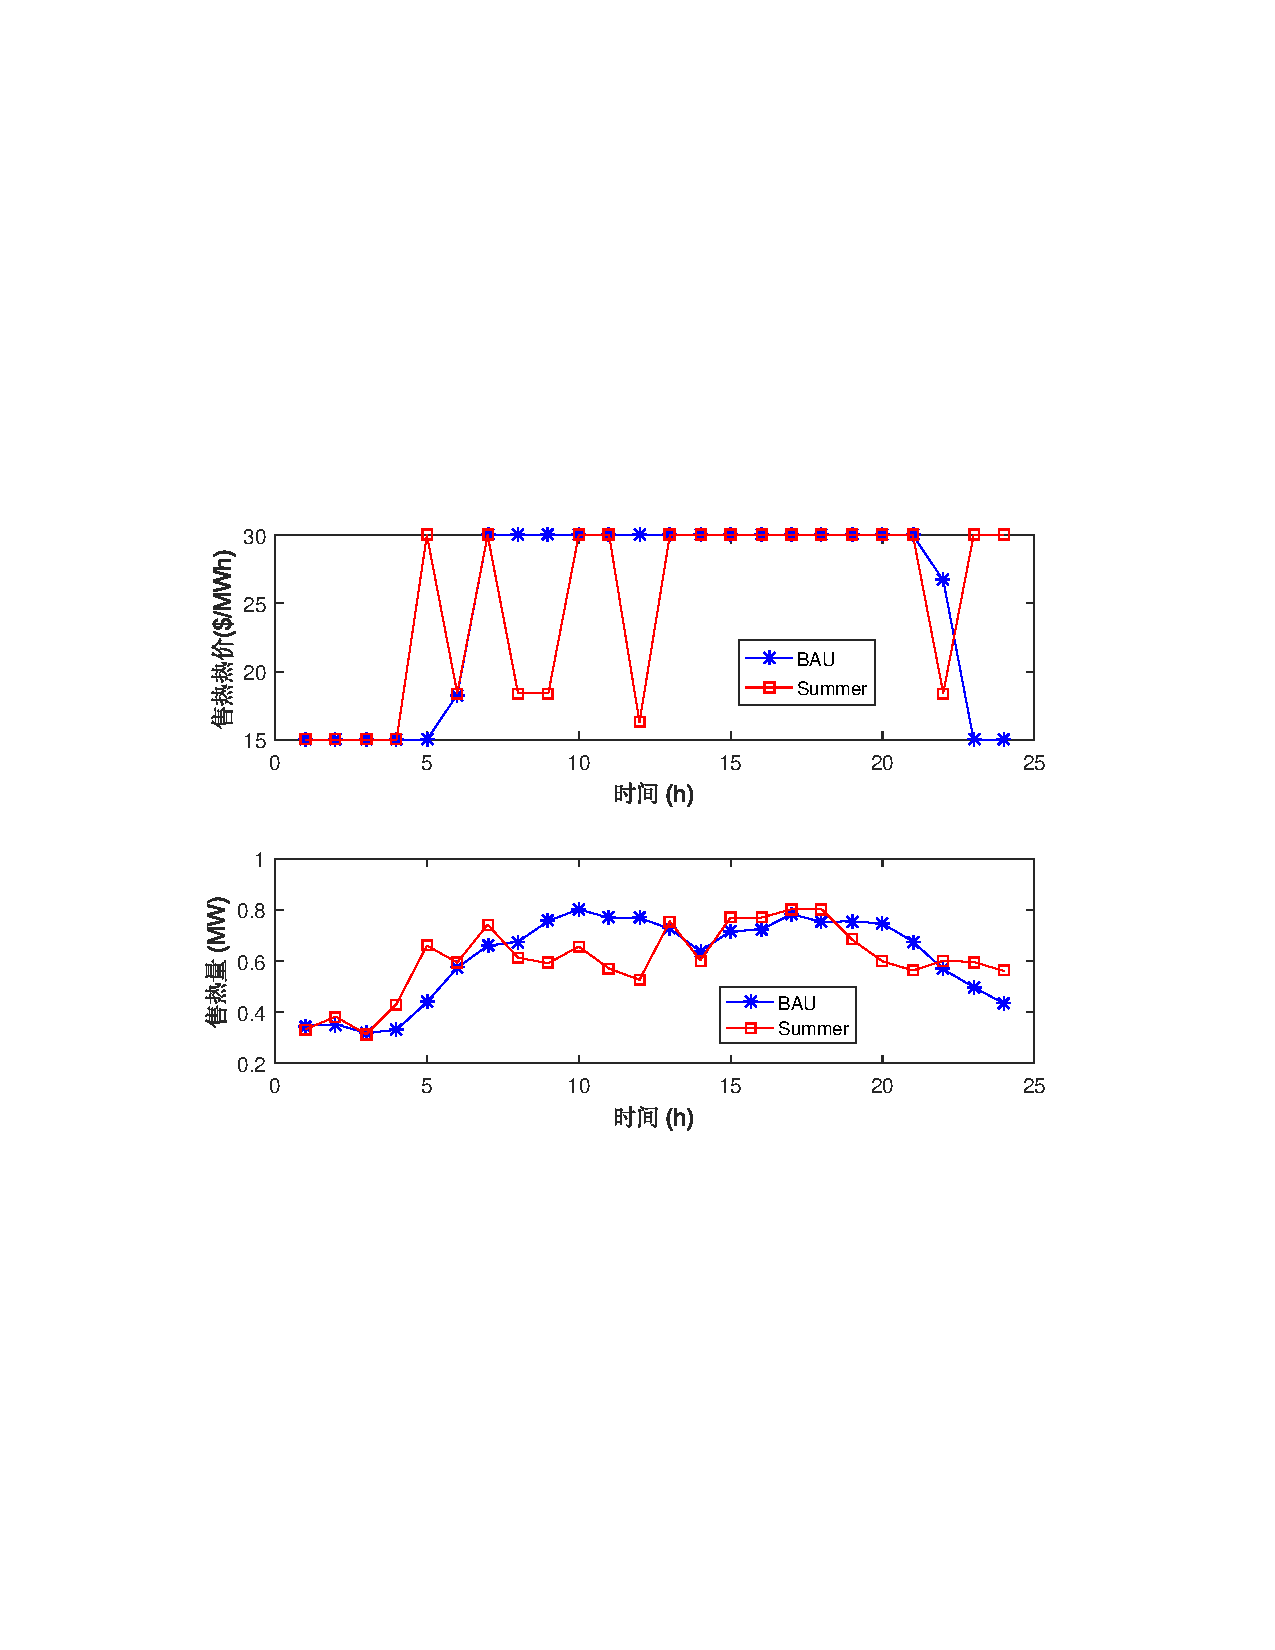
\includegraphics[scale=0.75]{figures/Chap4-13-HeatBidComp.pdf}
\caption{算例BEN与Summer热力市场竞标标的}
\label{Fig:HeatBidComp}
\end{figure}

\subsubsection{储能效率的影响}
在本小节算例中,电价曲线采用图\ref{Fig:GridPrice}中的TOU电价,储热效率设置为98$\%$。 AA-CAES电-电循环效率随不同的实现方式及技术成熟度发生变化,计算结果列于表~\ref{tab:SenResults}中。从表中可以发现,$\eta_{+}^{esu}>70\%$时,AA-CAES的电-电效率对能量枢纽整体利润有较大影响;当效率进一步降低时,效率对利润的减少几乎没有影响,其原因在于此时能量枢纽通过电力市场电价进行套利的收入将维持稳定,电力市场的主要收益源于消耗燃气的CHP出售电力。从表\ref{tab:SenResults}的后三行可知,由于储能效率较低,能量枢纽需要购买更多电力以实现一定的套利。因此,我们可以认为只有当AA-CAES的电-电循环效率高于49\%时,在不发挥AA-CAES本身的热电联供能力的条件下构建图\ref{fig:AA-CAES-Hub-V2}所示的II型AA-CAES是经济可行的;当AA-CAES的电-电效率低于49\%的条件下,用AA-CAES构建热电能量枢纽时应采用类似I型AA-CAES 的方案,以充分挖掘AA-CAES具有的供能灵活性。

\begin{table}[!t]
\scriptsize
\renewcommand{\arraystretch}{1.3}
\renewcommand{\tabcolsep}{1em}
\caption{不同储电效率下的能量枢纽收益 ($\$$)}
\centering
\begin{tabular}{cccccc}
\toprule
$\eta_{+}^{esu}/\eta_{-}^{esu}$ & {PDN成本}& {Gas成本} & {PDN收入} & {DHN收入} & {总利润}\\
\midrule
%98\%   & 331.07   & 489.72   & 993.02   & 397.77   & 569.99 \\
%95\%   & 330.55   & 528.97   & 993.02   & 397.77   & 531.27 \\
90\%   & 310.78   & 594.93   & 993.02   & 395.98   & 483.29 \\
85\%   & 313.13   & 605.99   & 946.48   & 394.68   & 425.72 \\
80\%   & 315.78   & 493.53   & 787.64   & 397.66   & 375.98 \\
75\%   & 318.78   & 493.53   & 749.08   & 398.38   & 335.15 \\
70\%   & 63.41    & \textbf{493.53}   & \textbf{474.94}   & \textbf{398.39}   & 316.39 \\
65\%   & 67.18    & \textbf{493.53}   & \textbf{474.94}   & \textbf{398.39}   & 312.62 \\
60\%   & 72.98    & \textbf{493.53}   & \textbf{474.94}   & \textbf{398.39}   & 306.82 \\
\bottomrule
\end{tabular}
\label{tab:SenResults}
\end{table}

\subsubsection{市场力测试与限制}
与市场力测试相关的算例分析结果如图\ref{Fig:MPGasIn}至图\ref{Fig:MPPriceE}所示。通过在算例{MP-GasLim}中对最大燃料输入功率进行限制,与算例{BEN}相比,能量枢纽在白天消耗更少的燃气,并在时段24购入更多的电量(图\ref{Fig:MPPInOut})。由图\ref{Fig:MPPriceE}可知,由于售电价较高,{BEN}与{MP-GasLim}两个算例的总收益差别不大($\$$469.48 v.s. $\$$466.44),而热力市场的收益是一样的,如附录\ref{cha:aa-caes-case-append}中表\ref{tab:MPResults}所示。

\begin{figure}[!htp]
\centering
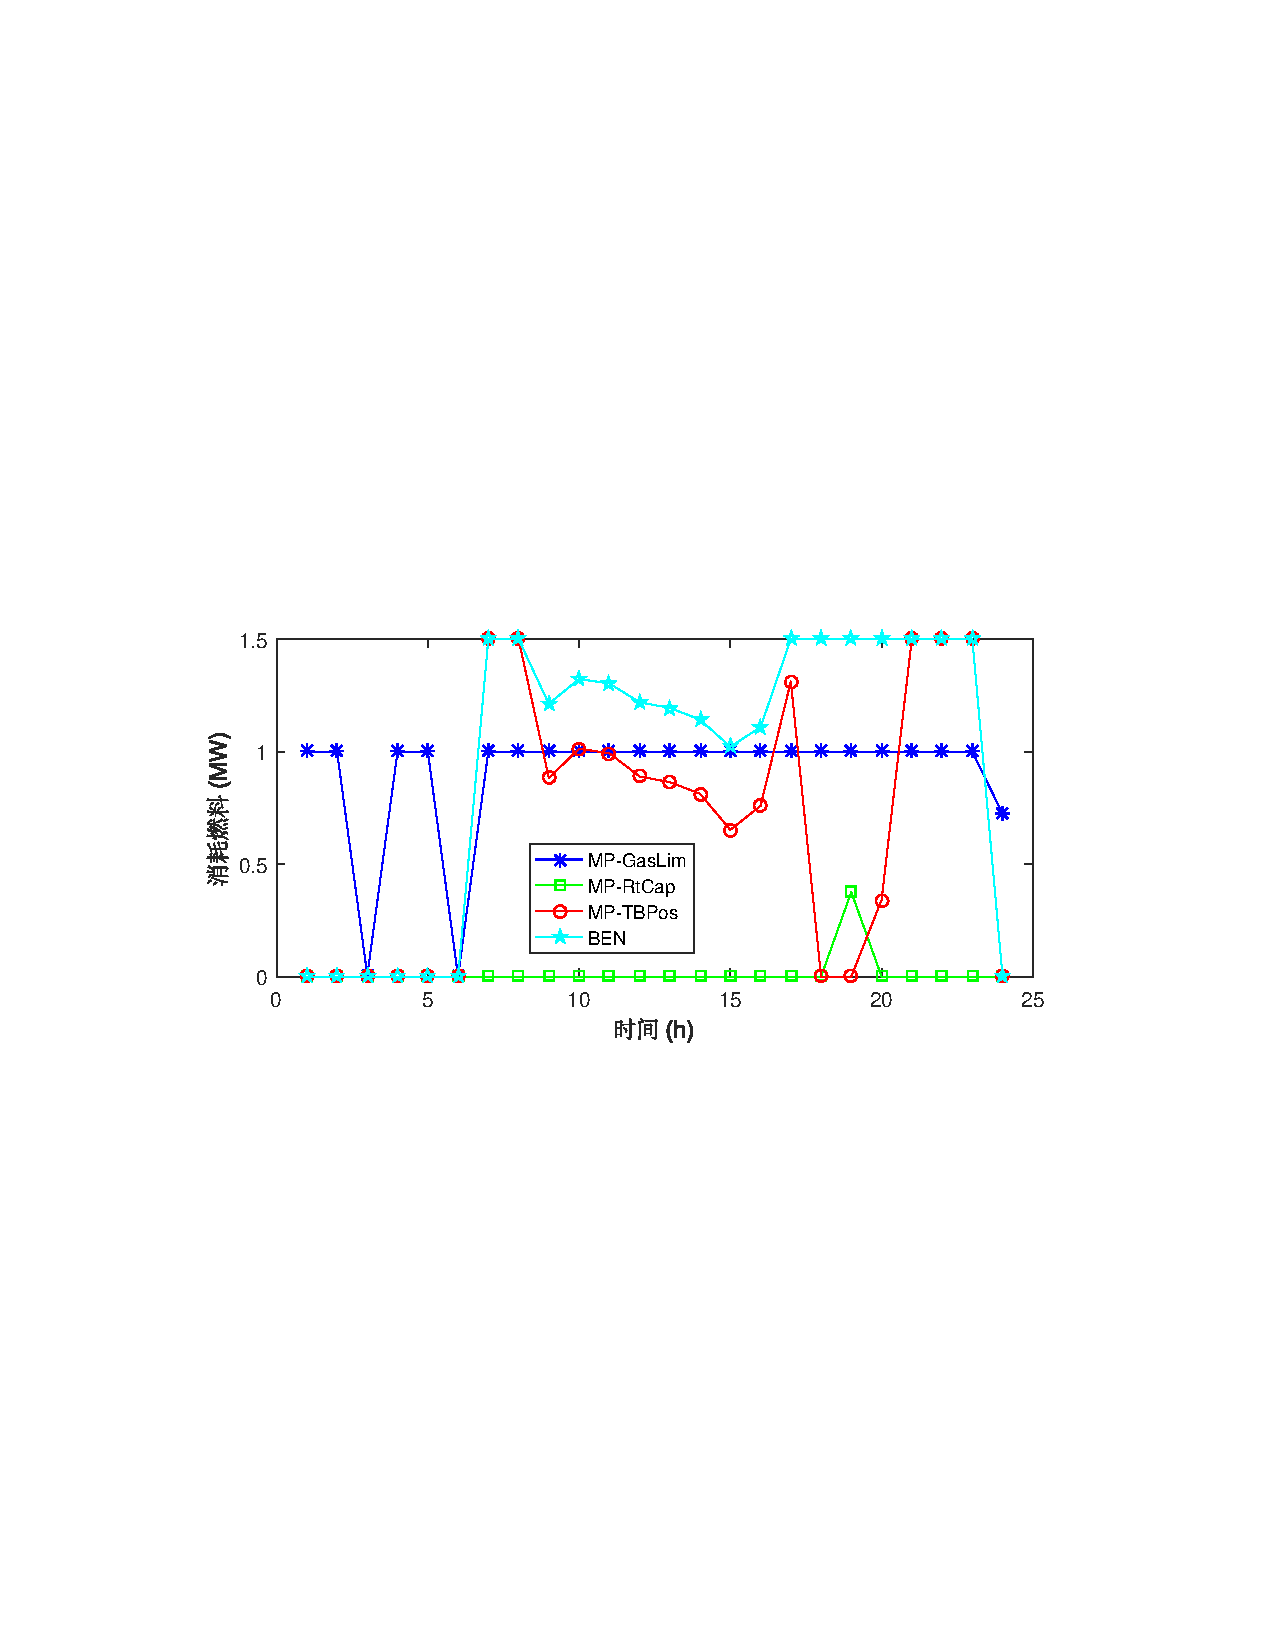
\includegraphics[scale=0.67]{figures/Chap4-14-MPCompGas.pdf}
\caption{市场力测试算例对应的燃料输入}
\label{Fig:MPGasIn}
\end{figure}

在算例{MP-TBPos}中,GT1有足够的容量来满足电力高峰时段的需求,因此时段9-17其售电量标的($p_{t,m}^{gb}$)比算例{BEN}中低,如图~\ref{Fig:MPPInOut}所示。相比于算例{MP-GasLim},由于峰值时刻出售的电量减少,{MP-TBPos}算例中购入的燃气也相应减少,在低谷时期(时段1-时段6)购买了更多的电量,以平衡购气量的减少,如图
\ref{Fig:MPGasIn}所示。此外,在算例{MP-TBPos},由于GTs出售了更多的电量,能量枢纽的售电标的($\xi^b$)在时段~18~低于算例{BEN}。
\begin{figure}[!htp]
\centering
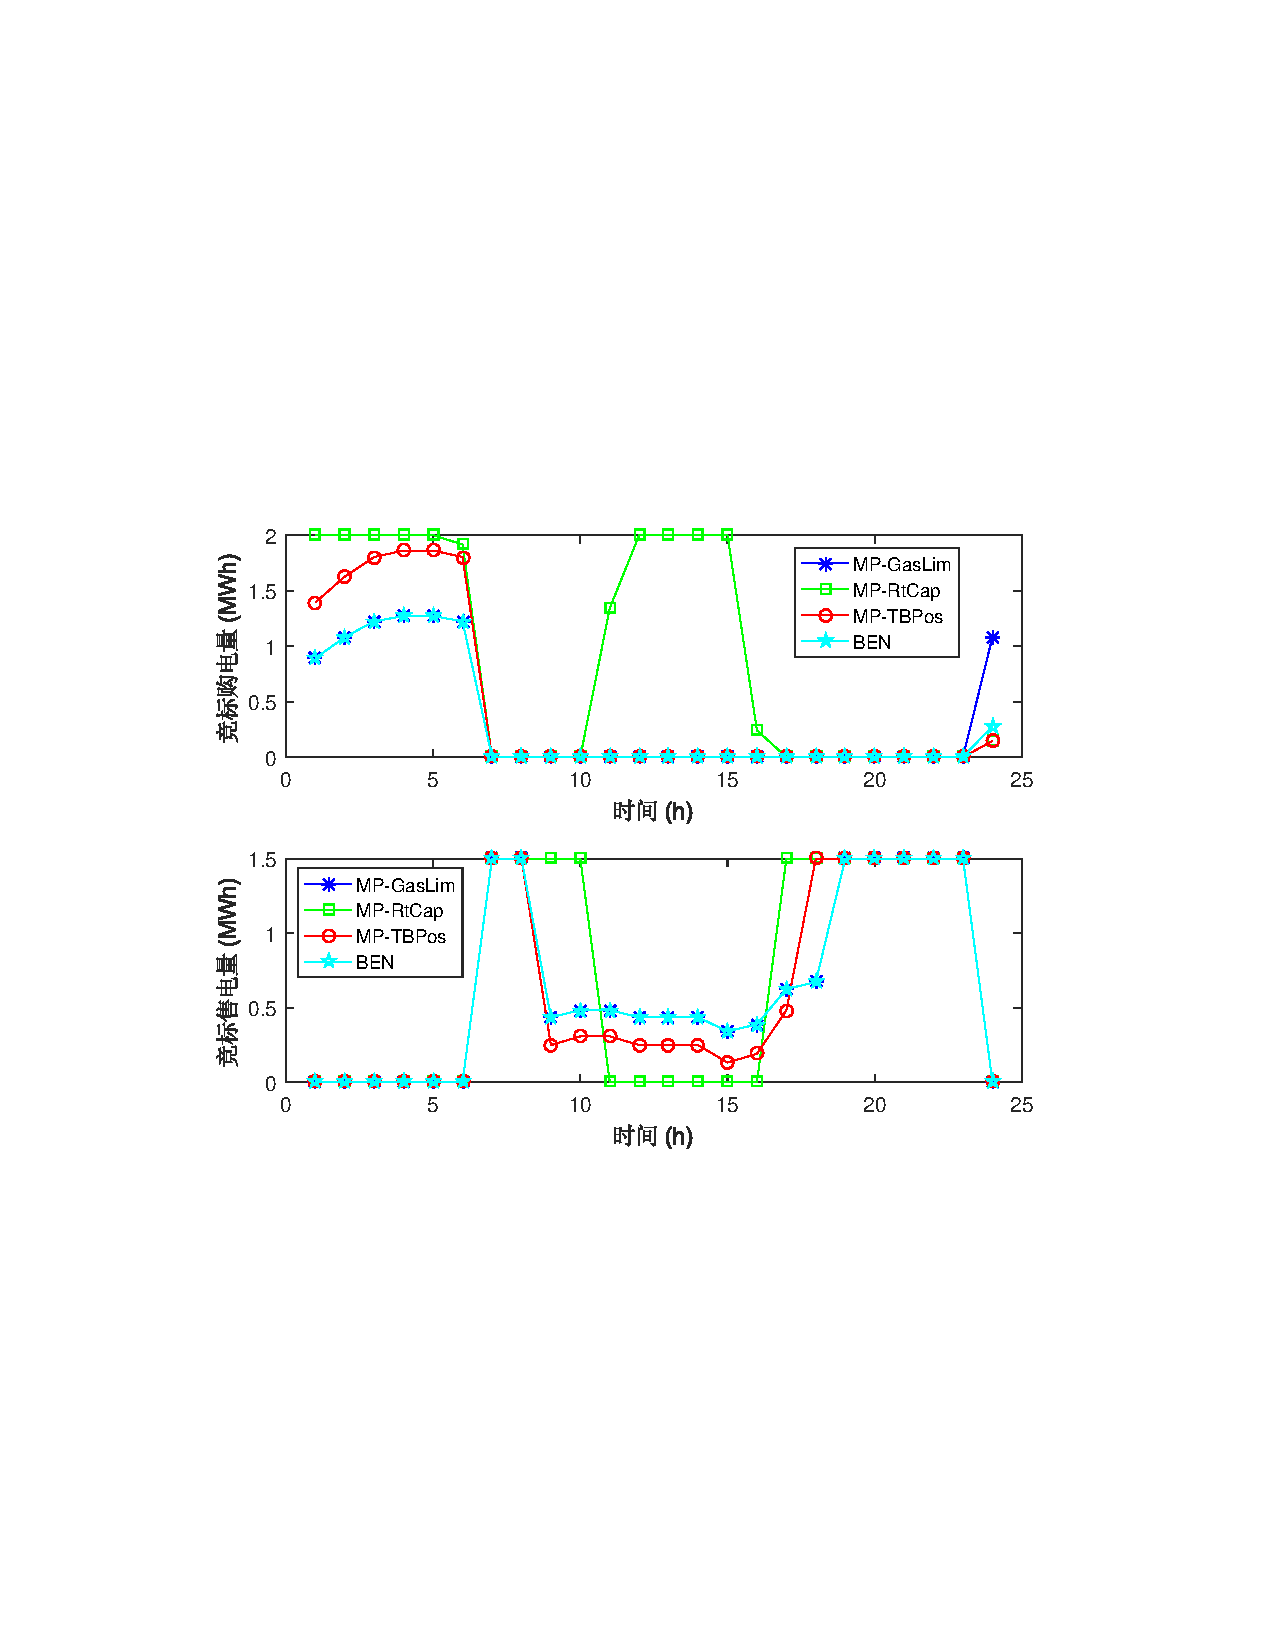
\includegraphics[scale=0.70]{figures/Chap4-15-MPComElQuan.pdf}
\caption{市场力测试算例集对应的售购电量竞标标的}
\label{Fig:MPPInOut}
\end{figure}
\begin{figure}[!htp]
\centering
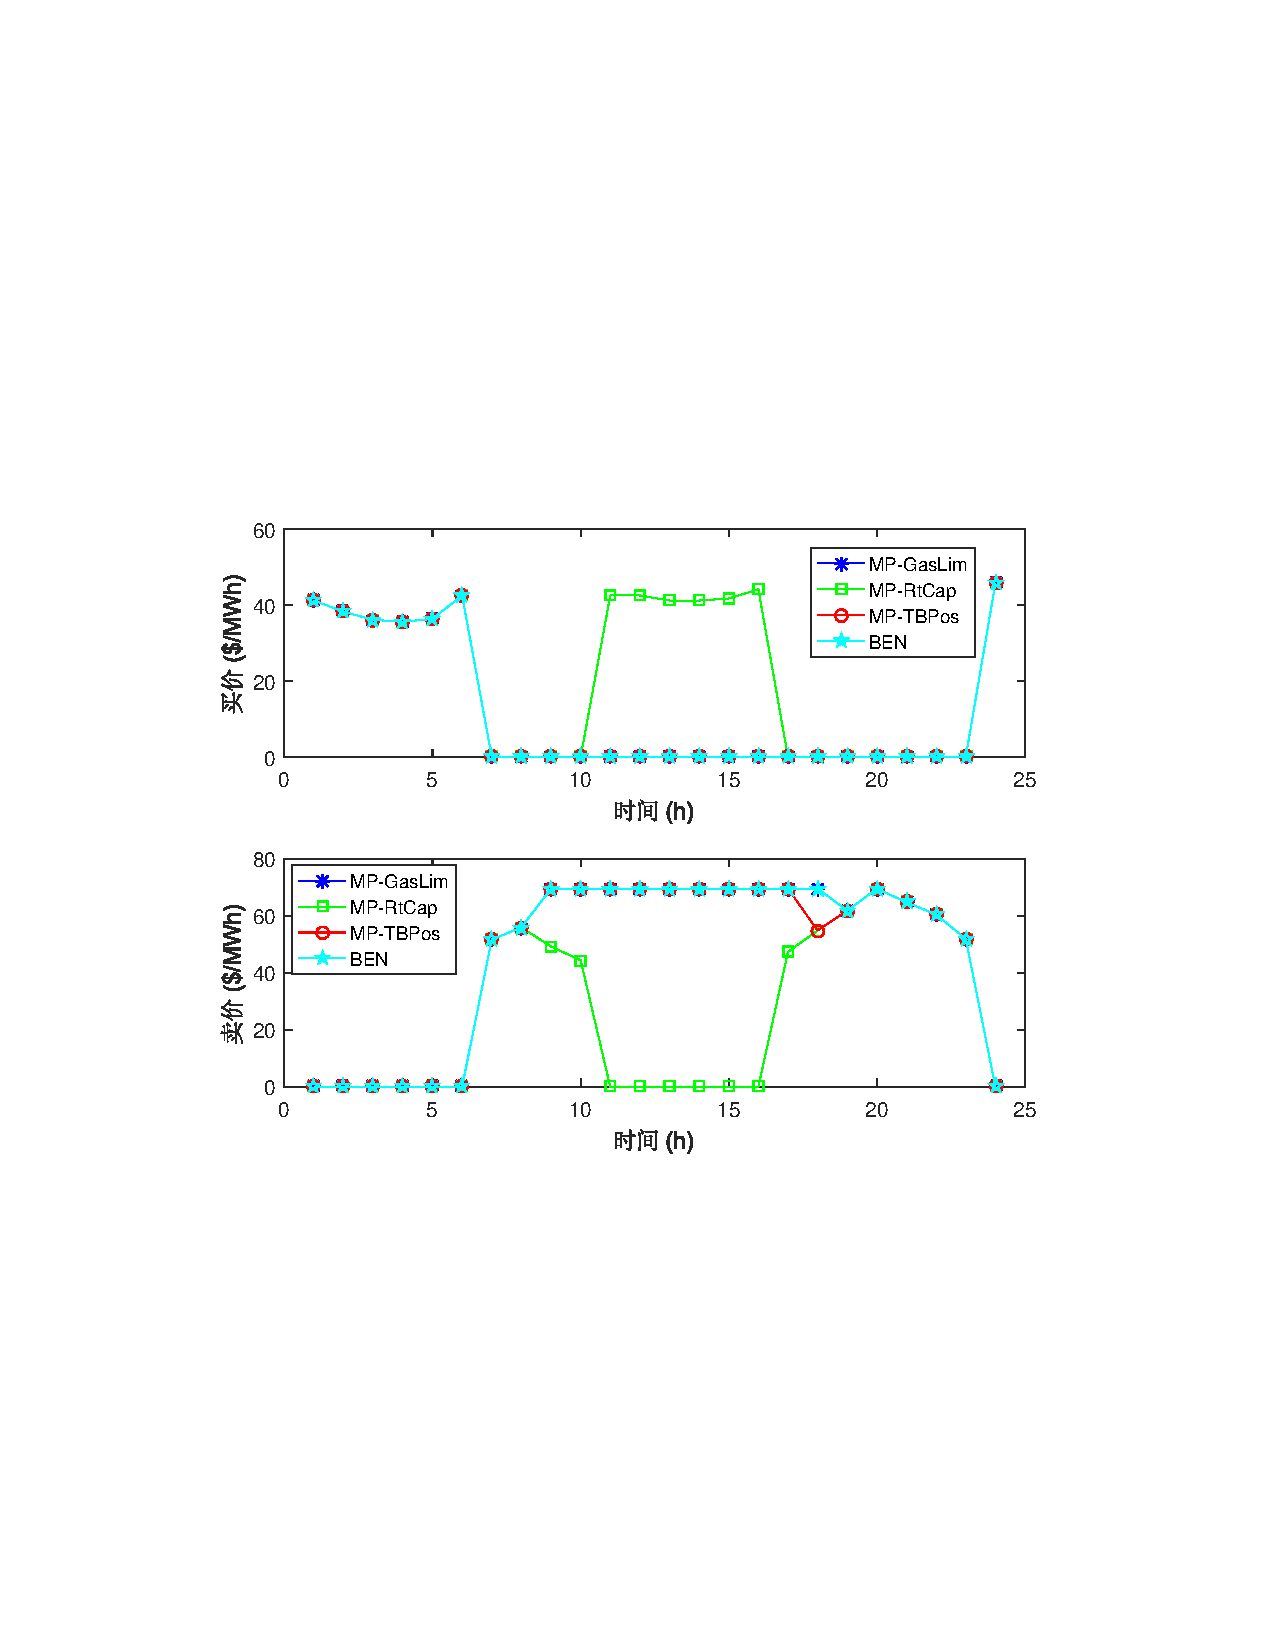
\includegraphics[scale=0.71]{figures/Chap4-16-MPCompElPrice.pdf}
\caption{市场力测试算例集对应的售购电价竞标标的}
\label{Fig:MPPriceE}
\end{figure}
限制能量枢纽市场力的另外一种方式是增加馈线容量,即连接上级电网的配电线路容量。在算例{MP-RtCap}中,由于来自上级电力市场的更加便宜的电量被输入到配电网中,能量枢纽丢失了一定的市场份额,同时购买了很少的燃气,如图~\ref{Fig:MPGasIn}所示。由于更多的电量从上级电网输送到配电网,为了确保一定的收益,相比于其它算例,能量枢纽转向降低售电电价标的,如时段9、10、16、17(见图\ref{Fig:MPPriceE})。此外,由于算例{MP-RtCap}中购买的燃气减少(见图\ref{Fig:MPGasIn}),热能仅能通过~HP~消耗电力产生,在时段1-7及时段11-16能量枢纽转向购买更多的电力来供应热负荷。因此,{MP-RtCap}算例中电力套利是II型AA-CAES能量枢纽的主要收益源。

%\section{基于AA-CAES能量枢纽的区域综合能源系统实例}
%\label{sec:AA-CAES-Micro-Energy-Grid}
%本节给出如图~\ref{Fig:IES-AA-CAES-Hub1}所示的基于I型AA-CAES能量枢纽与图~\ref{Fig:IES-AA-CAES-Hub2}所示的II型AA-CAES能量枢纽的两类区域综合能源系统结构实现形式。

%\begin{figure}[!htp]
%\centering
%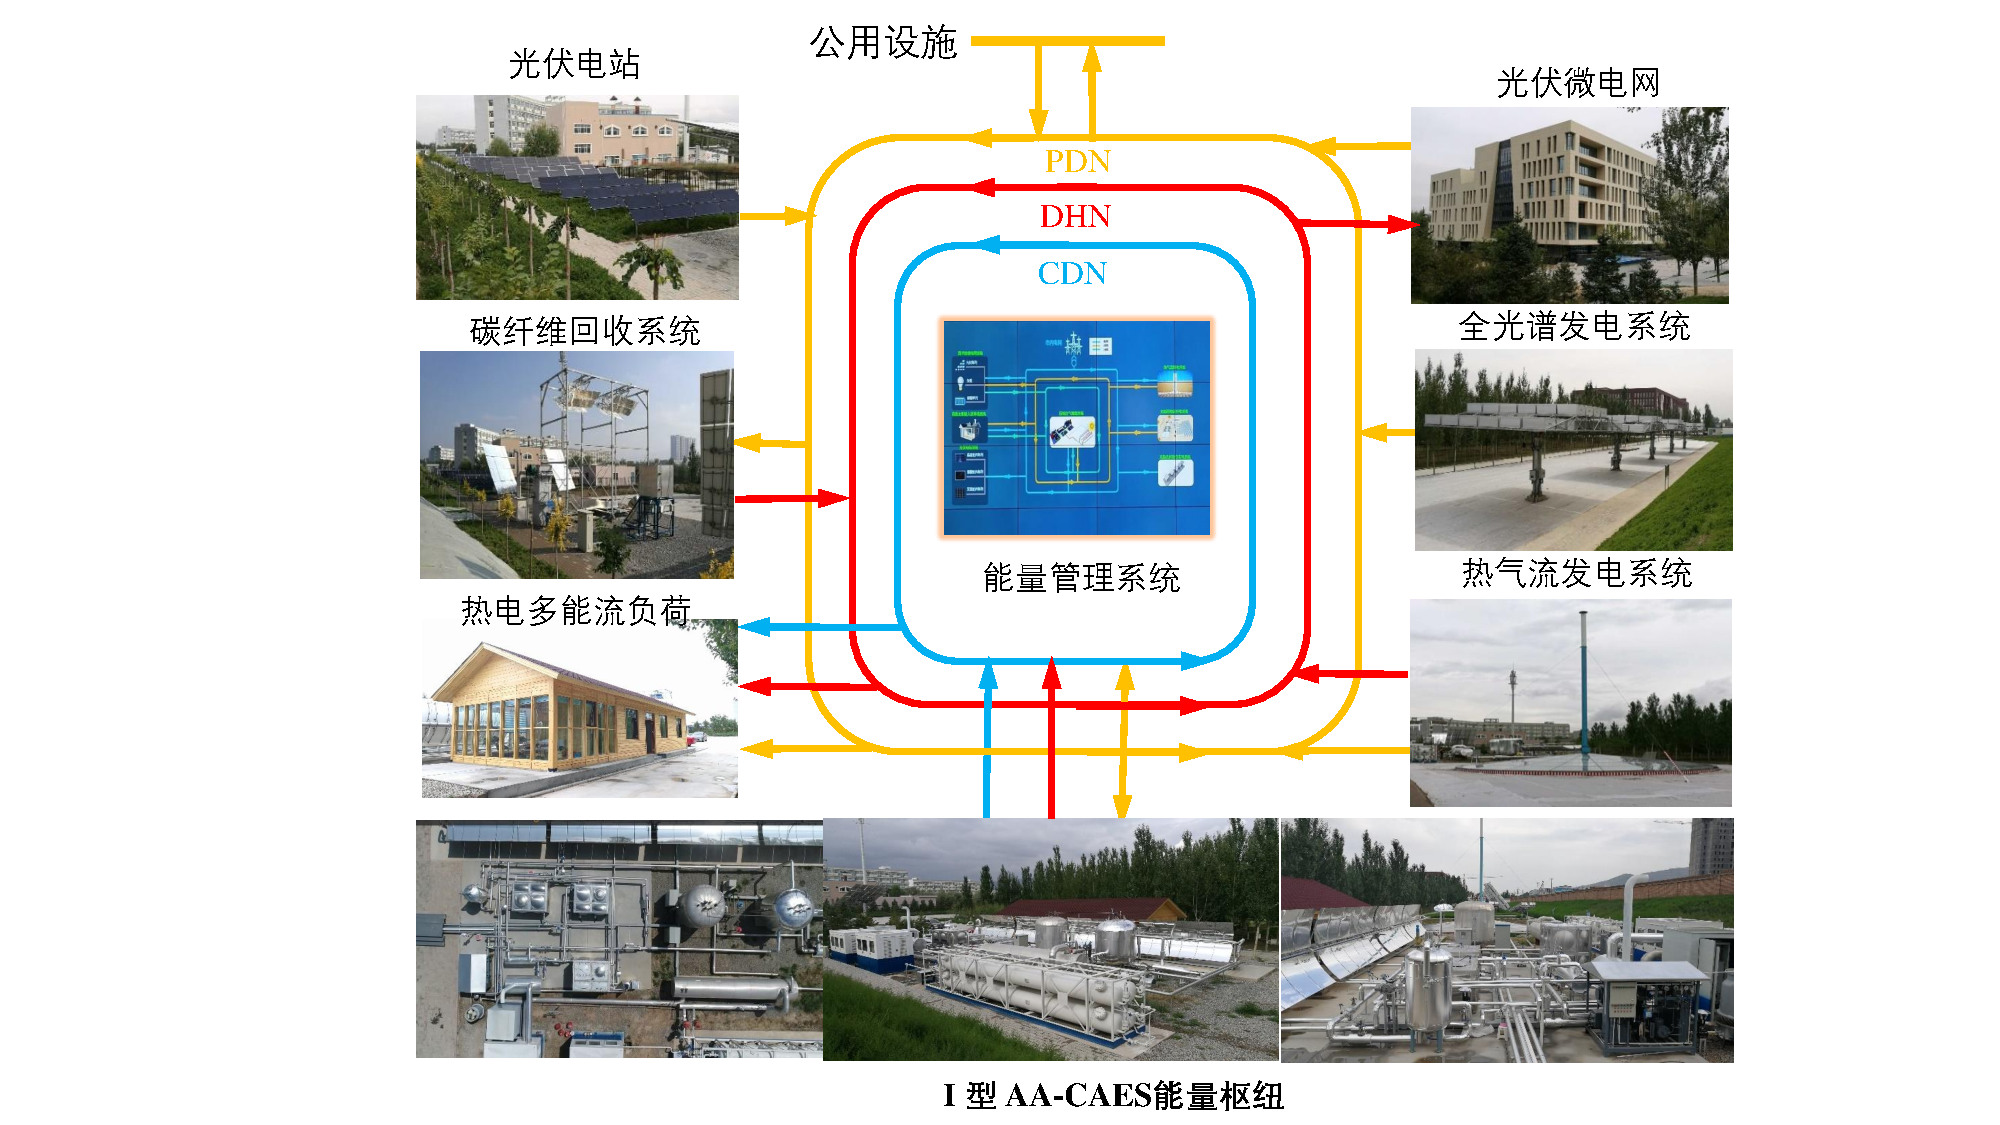
\includegraphics[scale=0.45]{figures/Chap4-20-IES-AA-CAES-Hub1.pdf}
%\caption{基于I 型 AA-CAES能量枢纽的区域综合能源系统}
%\label{Fig:IES-AA-CAES-Hub1}
%\end{figure}

%\begin{figure}[!htp]
%\centering
%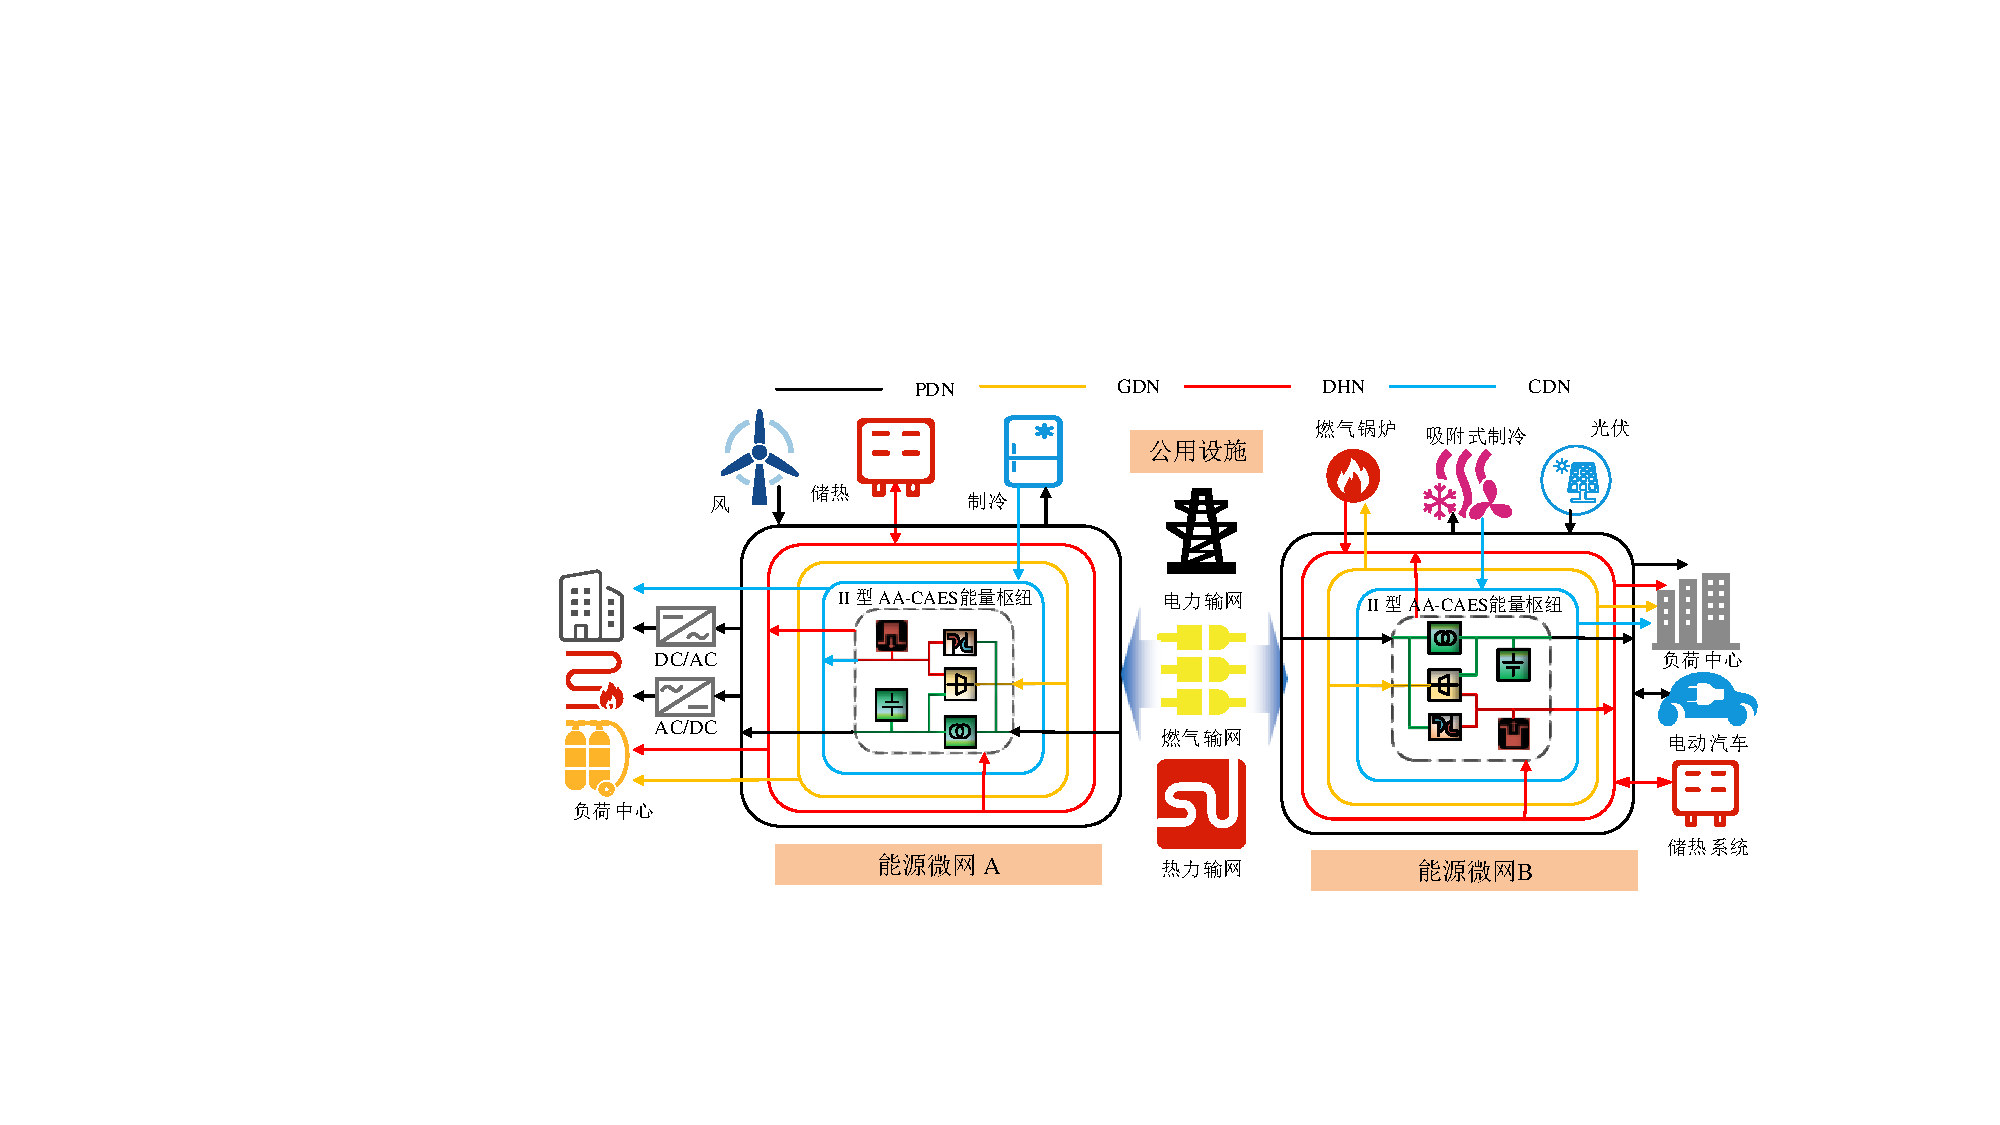
\includegraphics[scale=0.70]{figures/Chap4-20-IES-AA-CAES-Hub2.pdf}
%\caption{基于II 型 AA-CAES能量枢纽的区域综合能源系统}
%\label{Fig:IES-AA-CAES-Hub2}
%\end{figure}

\section{小结}
不同于电池储能与抽蓄储能等,AA-CAES由于蓄热系统的存在具备了热电联供与热电联储的能力,具备了供能灵活性,使其成为一类天然的热电互补能量枢纽。本章针对两类典型的AA-CAES型能量枢纽的建模设计、最优调度及市场竞标展开研究,以灵活负荷的形式为可再生能源系统注入灵活资源。
